\documentclass[letterpaper]{article}
\usepackage[margin=1in]{geometry}
\usepackage[utf8]{inputenc}
\usepackage{textcomp}
\usepackage{amssymb}
\usepackage{natbib}
\usepackage{graphicx}
\usepackage{gensymb}
\usepackage{amsthm, amsmath, mathtools}
\usepackage[dvipsnames]{xcolor}
\usepackage{enumerate}
\usepackage{mdframed}
\usepackage[most]{tcolorbox}
\usepackage{csquotes}
% https://tex.stackexchange.com/questions/13506/how-to-continue-the-framed-text-box-on-multiple-pages

\tcbuselibrary{theorems}

\newcommand{\R}{\mathbb{R}}
\newcommand{\Z}{\mathbb{Z}}
\newcommand{\N}{\mathbb{N}}
\newcommand{\Q}{\mathbb{Q}}
\newcommand{\C}{\mathbb{C}}
\newcommand{\code}[1]{\texttt{#1}}
\newcommand{\mdiamond}{$\diamondsuit$}
\newcommand{\PowerSet}{\mathcal{P}}
\newcommand{\Mod}[1]{\ (\mathrm{mod}\ #1)}
\DeclareMathOperator{\lcm}{lcm}

%\newtheorem*{theorem}{Theorem}
%\newtheorem*{definition}{Definition}
%\newtheorem*{corollary}{Corollary}
%\newtheorem*{lemma}{Lemma}
\newtheorem*{proposition}{Proposition}


\newtcbtheorem[number within=section]{theorem}{Theorem}
{colback=green!5,colframe=green!35!black,fonttitle=\bfseries}{th}

\newtcbtheorem[number within=section]{definition}{Definition}
{colback=blue!5,colframe=blue!35!black,fonttitle=\bfseries}{def}

\newtcbtheorem[number within=section]{corollary}{Corollary}
{colback=yellow!5,colframe=yellow!35!black,fonttitle=\bfseries}{cor}

\newtcbtheorem[number within=section]{lemma}{Lemma}
{colback=red!5,colframe=red!35!black,fonttitle=\bfseries}{lem}

\newtcbtheorem[number within=section]{example}{Example}
{colback=white!5,colframe=white!35!black,fonttitle=\bfseries}{def}

\newtcbtheorem[number within=section]{note}{Important Note}{
        enhanced,
        sharp corners,
        attach boxed title to top left={
            xshift=-1mm,
            yshift=-5mm,
            yshifttext=-1mm
        },
        top=1.5em,
        colback=white,
        colframe=black,
        fonttitle=\bfseries,
        boxed title style={
            sharp corners,
            size=small,
            colback=red!75!black,
            colframe=red!75!black,
        } 
    }{impnote}
\usepackage[utf8]{inputenc}
\usepackage[english]{babel}
\usepackage{fancyhdr}
\usepackage[hidelinks]{hyperref}

\pagestyle{fancy}
\fancyhf{}
\rhead{CSE 105}
\chead{March 9th, 2022}
\lhead{Course Notes}
\rfoot{\thepage}

\setlength{\parindent}{0pt}

\begin{document}

\begin{titlepage}
    \begin{center}
        \vspace*{1cm}
            
        \Huge
        \textbf{CSE 105}
            
        \vspace{0.5cm}
        \LARGE
        Theory of Computability
            
        \vspace{1.5cm}
        
        \begin{center}
            
\includegraphics[]{assets/genie.png}
        \end{center}
        \vfill
            
        Winter 2022 \\
        Taught by Professor Shachar Lovett
    \end{center}
\end{titlepage}

\pagenumbering{gobble}

\newpage 

\pagenumbering{gobble}
\begingroup
    \renewcommand\contentsname{Table of Contents}
    \tableofcontents
\endgroup

\bigskip 

\textbf{Remark:} A lot of the pictures and explanations were taken from \emph{Introduction to the Theory of Computation} (3rd Edition) by Michael Sipser and from the CSE 105 lecture slides. 

\newpage
\pagenumbering{arabic}

\section{Strings and Languages (Review)}
\begin{definition}{Alphabet}{}
    An \textbf{alphabet} is any nonempty finite set. Generally, we use $\Sigma$ and $\Gamma$ to designate alphabets.
\end{definition}

\begin{definition}{Symbols}{}
    The members of the alphabet are the \textbf{symbols} of the alphabet.
\end{definition}

Some example of alphabets are: 
\[\Sigma_1 = \{\code{0, 1}\}\]
\[\Sigma_2 = \{\code{a, b, c, d, e, f, g, h, i, j, k, l, m, n, o, p, q, r, s, t, u, v, w, x, y, z}\}\]
\[\Gamma = \{\code{0, 1, x, y, z}\}\]

\begin{definition}{String}{}
    A \textbf{string} over an alphabet is a finite sequence of symbols from that alphabet, usually written next to one another and not separated by commas. 
\end{definition}
For example, if we use $\Sigma_1$ as our alphabet, then \code{01001} is a \textbf{string} over $\Sigma_1$. Likewise, if we use $\Sigma_2$ as our alphabet, then \code{something} is a string over $\Sigma_2$. 

\bigskip

The set of all finite strings over $\Sigma$ (any general alphabet) is denoted by $\Sigma^*$. Here, this includes:
\begin{itemize}
    \item The empty string $\epsilon$.
    \item Any \textbf{finite} combination of the symbols in this alphabet.
\end{itemize}
This does not include infinite sequences of symbols. It does have infinitely many elements. 

\bigskip

So, for example, $\Sigma_{1}^{*}$ would have strings like (and keep in mind that these are just examples): 
\[\epsilon \in \Sigma_{1}^{*} \qquad \code{0} \in \Sigma_{1}^{*} \qquad \code{1} \in \Sigma_{1}^{*}\]
\[\code{010101} \in \Sigma_{1}^{*} \qquad \code{1111} \in \Sigma_{1}^{*} \qquad \code{0000} \in \Sigma_{1}^{*}\]

\begin{definition}{Length}{}
    If $w$ is a string over $\Sigma$, then the \textbf{length} of $w$, written $|w|$, is the number of symbols that it contains. 
\end{definition}
\textbf{Remarks:}
\begin{itemize}
    \item The string of length zero is called the \textbf{empty string} and is written $\epsilon$. The empty string plays the role of 0 (like an identity) in a number system.
    \item If $w$ has length $n$, then we can write $w = w_1 w_2 \dots w_n$ where each $w_i \in \Sigma$.
\end{itemize} 

\begin{definition}{Reverse}{}
    The \textbf{reverse} of a string $w$, written $w^{\mathcal{R}}$, is the string obtained by writing $w$ in the opposite order.
\end{definition}
\textbf{Remark:} In other words, for a string $w$, we can write the reverse of $w$ as $w^{\mathcal{R}} = w_n w_{n - 1} \dots w_{2} w_{1}$. 

\begin{definition}{Substring}{}
    A string $z$ is a \textbf{substring} of a string $w$ if $z$ appears consecutively within $w$.
\end{definition}
For example, if we look at the string $w = \code{something}$, then $z_1 = \code{some}$ and $z_2 = \code{thing}$ are both substrings of $w$. 

\begin{definition}{Concatenation}{}
    For a string $x$ of length $m$ and a string $y$ of length $n$, the \textbf{concatenation} of $x$ and $y$, written $xy$, is the string obtained by appending $y$ to the end of $x$, as in: 
    \[x_1 \dots x_m y_1 \dots y_n\]
    If we want to concatenate a string $x$ with itself many times, we use the superscript notation $x^k$ to mean: 
    \[\underbrace{xx \dots x}_{k}\]
\end{definition}
If we consider the two substrings $z_1$ and $z_2$ in the previous example, then $z_1 z_2 = \code{something}$. 

\begin{definition}{Prefix}{}
    A string $x$ is a \textbf{prefix} of a string $y$ if a string $z$ exists where $xz = y$.
\end{definition}
For example, if we look at the two substrings $z_1$ and $z_2$ in the previous example yet again, we say that $z_1$ is a prefix of $w$ since $z_1 z_2 = w$. 

\begin{definition}{Proper Prefix}{}
    A string $x$ is a proper prefix of a string $y$ if, in addition to $x$ being a prefix of $y$, $x \neq y$.
\end{definition}
So, \code{some} is a proper prefix of \code{something} while \code{something} is not a proper prefix of \code{something}.

\begin{definition}{Language}{}
    A \textbf{language} is a set of strings. 
\end{definition}

\begin{definition}{Prefix-Free}{}
    A language is \textbf{prefix-free} if no member is a proper prefix of another member.
\end{definition}









































\newpage 
\section{Finite Automata (1.1)}
Consider the controller for an automatic one-way door.
\begin{center}
    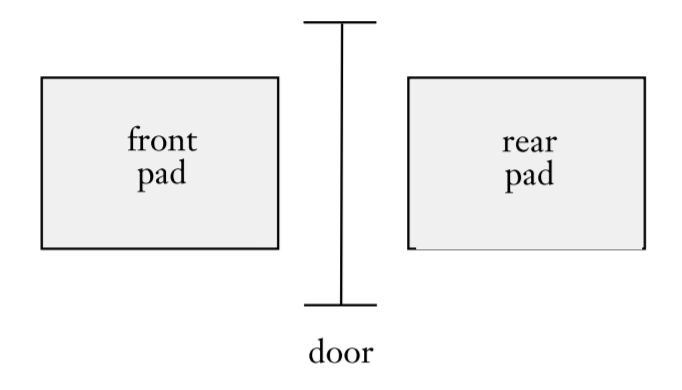
\includegraphics[scale=0.4]{assets/door.png}
\end{center}
Here:
\begin{itemize}
    \item The front pad is there is to detect the presence of a person who is about to walk through the doorway. 
    \item The rear pad is there so that the controller can hold the door open long enough for the person to pass all the way through while also ensuring that no one behind door is hit by the door. 
\end{itemize}
The controller is in either of two states: \code{OPEN} or \code{CLOSED}. This represents the condition of the door. There are also \emph{four} possible input conditions: 
\begin{itemize}
    \item \code{FRONT}: A person is standing on the pad in front of the doorway (the front pad).
    \item \code{REAR}: A person is standing on the pad to the rear of the doorway (the rear pad).
    \item \code{BOTH}: People are standing on both pads. 
    \item \code{NEITHER}: No one is standing on either pad.
\end{itemize}
The corresponding state diagram is: 
\begin{center}
    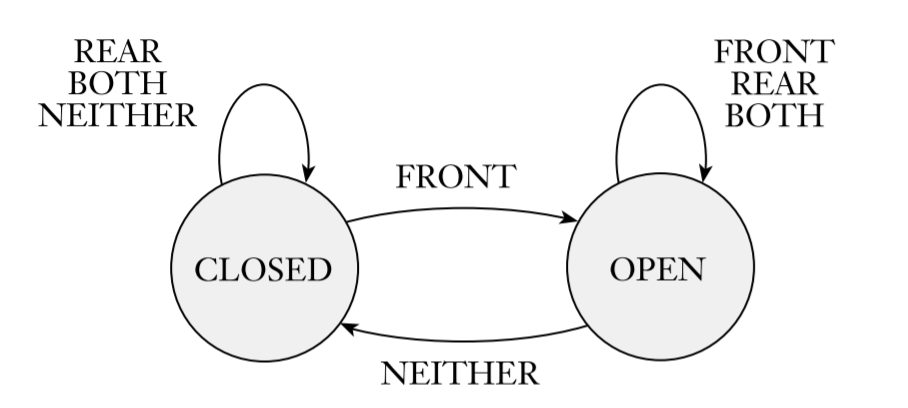
\includegraphics[scale=0.4]{assets/door_state.png}
\end{center}
And the corresponding transition table: 
\begin{center}
    \begin{tabular}{c|c c c c} 
                & \code{NEITHER} & \code{FRONT} & \code{REAR} & \code{BOTH} \\ 
            \hline
            \code{CLOSED} & \code{CLOSED} & \code{OPEN} & \code{CLOSED} & \code{CLOSED} \\ 
            \code{OPEN} & \code{CLOSED} & \code{OPEN} & \code{OPEN} & \code{OPEN} 
    \end{tabular}
\end{center}

The controller moves from state to state depending on what input it receives. For example: 
\begin{itemize}
    \item When it starts off in the \code{CLOSED} state and receives input \code{NEITHER} or \code{REAR}, it remains in the \code{CLOSED} state. In the state diagram, if we start at the \code{CLOSED} circle (state), both \code{NEITHER} and \code{REAR} loop back to \code{CLOSED}.
    \item Again, when the controller is in the \code{CLOSED} state and it receives the \code{BOTH} input, then it stays in the \code{CLOSED} state because opening the door may knock someone over on the rear pad (as the door opens towards the rear side).
    \item If the controller is in the \code{OPEN} state, then receiving the inputs \code{FRONT}, \code{REAR}, or \code{BOTH} will result in the controller remaining \code{OPEN}. However, if it receives the \code{NEITHER} input, then it goes to a \code{CLOSED} state. 
\end{itemize}
Essentially, \textbf{for the state diagram}, start at the initial state (circle) and follow the arrow depending on what input signals are received. \textbf{For the transition table}, look at the row corresponding to the initial state and the column corresponding to the input; the resulting cell will be the new state of the controller.

\bigskip

The figures used above (the state diagram and transition table) are both standard ways of representating a finite automaton. While this door may be very simple (due to the fact that it only really needs to store an extremely small amount of memory), in reality, we may be dealing with other devices with somewhat more memory. 

\bigskip

Both finite automata and their probablistic counterpart \textbf{Markov chains} are useful tools when we want to attempt to recognize patterns in data. 

\subsection{From a Mathematical Perspective}
Consider the following figure, which depicts a finite automaton called $M_1$:
\begin{center}
    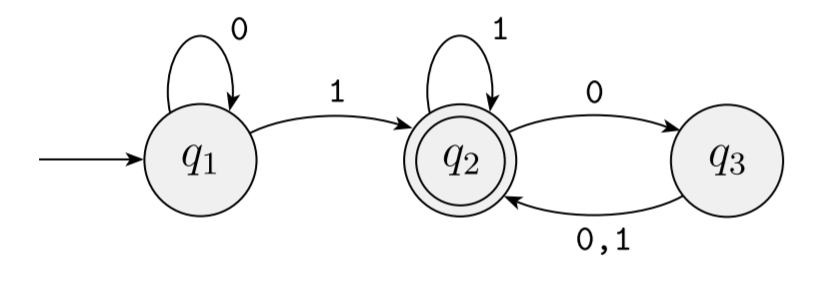
\includegraphics[scale=0.4]{assets/finite_automaton_1.png}
\end{center}
There are a few things to note here: 
\begin{itemize}
    \item The above figure for $M_1$ is called the \textbf{state diagram} of $M_1$. 
    \item $M_1$ has three \textbf{states}, labeled $q_1$, $q_2$, and $q_3$. 
    \item The \textbf{start state} is the state indicated by the arrow pointing at it from nowhere. In the case of the above state diagram, this would be $q_1$. 
    \item The \textbf{accept state} is the state with a \underline{double circle}. In the case of the above state diagram, this would be $q_2$. 
    \item The \textbf{transitions} are the arrows going from one state to another. 
\end{itemize}
For a given input string, \underline{this} automaton processes that string and produces an output that is either \code{ACCEPT} or \code{REJECT}. For this automaton, the processing works like so: 
\begin{enumerate}
    \item Here, the processing begins in $M_1$'s start state. 
    \item Then, the automaton receives the symbols from the input string one by one from left to right. 
    \item After reading each symbol, $M_1$ moves from one state to another along the transition that has that symbol as its label. 
    \item When it reads the last symbol, $M_1$ produces its output. The output is \code{ACCEPT} if $M_1$ is now in an accept state and \code{REJECT} if it is not. 
\end{enumerate}
As an example, suppose we give $M_1$ the input string \code{1101}. Then, the processing proceeds as follows: 
\begin{itemize}
    \item Start in state $q_1$. 
    \item Read \code{1}. Transition from $q_1$ to $q_2$. 
    \item Read \code{1}. Transition from $q_2$ to $q_2$. 
    \item Read \code{0}. Transition from $q_2$ to $q_3$. 
    \item Read \code{1}. Transition from $q_3$ to $q_2$. 
    \item \code{ACCEPT} because $M_1$ is in an accept state $q_2$ at the end of the input. 
\end{itemize}
So, really, what matters is that we \emph{end up} at the accept state. 

\subsection{Formal Definition of a Finite Automaton}
A finite automaton has several parts.
\begin{itemize}
    \item It has a set of states and rules for going from one state to another, depending on the input symbol.
    \item It has an input alphabet that indicates the allowed input symbols. 
    \item It has a start state and a set of accept states. 
\end{itemize}
We use something called a \textbf{transition function}, often denoted $\delta$, to define the rules for moving. If the finite automaton has an arrow from a state $x$ to a state $y$ labeled with the input symbol \code{1}, that means that if the automaton is in state $x$ when it reads a \code{1}, it then moves to state $y$. We can indicate the same thing with the transition function by saying that: 
\[\delta(x, \code{1}) = y\]
All of this leads to the formal definition:
\begin{definition}{Finite Automaton}{}
    A \textbf{finite automaton} is a 5-tuple $(Q, \Sigma, \delta, q_0, F)$ where: 
    \begin{enumerate}
        \item $Q$ is a finite set called the \textbf{states}.
        \item $\Sigma$ is a finite set called the \textbf{alphabet}.
        \item $\delta: Q \times \Sigma \mapsto Q$ is the \textbf{transition function}.
        \item $q_0 \in Q$ is the \textbf{start state}.
        \item $F \subseteq Q$ is the \textbf{set of accept states} (sometimes also called \emph{final states}).
    \end{enumerate}
\end{definition}
\textbf{Remark:} $F$ can be the empty set $\emptyset$, which means that there are 0 accept states.

\subsection{Applying the Definition}
Consider again $M_1$:
\begin{center}
    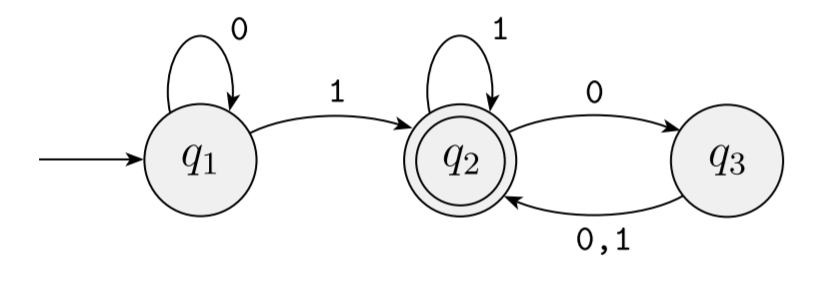
\includegraphics[scale=0.4]{assets/finite_automaton_1.png}
\end{center}
Using the formal definition above, we can describe $M_1$ formally be writing $M_1 = (Q, \Sigma, \delta, q_1, F)$, where: 
\begin{itemize}
    \item $Q = \{q_1, q_2, q_3\}$
    \item $\Sigma = \{\code{0, 1}\}$
    \item $\delta$ is defined as: 
    \begin{center}
        \begin{tabular}{c|c c}
                  & \code{0} & \code{1} \\ 
            \hline 
            $q_1$ & $q_1$    & $q_2$ \\ 
            $q_2$ & $q_3$    & $q_2$ \\ 
            $q_3$ & $q_2$    & $q_2$ 
        \end{tabular}
    \end{center}
    \item $q_1$ is the start state. 
    \item $F = \{q_2\}$. 
\end{itemize}

\subsection{Machine and Language}
If $A$ is the set of all strings (i.e. language) that machine $M$ accepts, we say that $A$ is the \textbf{language of machine} $M$, write $L(M) = A$, and say that $M$ recognizes $A$. 

\bigskip

A machine may accept \emph{several strings}, but it always recognizes \underline{one language}. A machine can accept no strings; in this case, it still recognizes the empty language $\emptyset$. 

\bigskip

If we consider our example automaton $M_1$, then define: 
\[A = \{w \mid w \text{ contains at least one \code{1} or an even number of \code{0}s follow the last \code{1}}\}\]
Which means that $L(M_1) = A$, of equivalently, $M_1$ recognizes $A$. 

\subsubsection{Example 1: Simple Finite Automaton}
Consider the following state diagram for the finite automaton $M_2$:
\begin{center}
    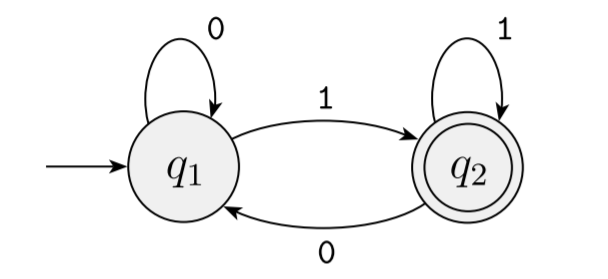
\includegraphics[scale=0.4]{assets/finite_automaton_2.png}
\end{center}
Here, the formal description of $M_2$ is as follows: 
\[M_2 = (\{q_1, q_2\}, \{\code{0, 1}\}, \delta, q_1, \{q_2\})\]
Where $\delta$ is: 
\begin{center}
    \begin{tabular}{c|c c}
            & \code{0} & \code{1} \\
        \hline  
        $q_1$ & $q_1$ & $q_2$ \\ 
        $q_2$ & $q_1$ & $q_2$
    \end{tabular}
\end{center}
To figure out what $A$ is, we try a few different strings.
\begin{center}
    \begin{tabular}{c|c}
        \textbf{String Input} & \textbf{Output} \\ 
        \hline 
        $\epsilon$ & \code{REJECT} \\ 
        \code{1} & \code{ACCEPT} \\ 
        \code{0} & \code{REJECT} \\ 
        \code{01} & \code{ACCEPT} \\ 
        \code{10} & \code{REJECT} \\ 
        \code{11} & \code{ACCEPT}
    \end{tabular}
\end{center}
It's quite clear that $A$ is simply the set of all strings that end with \code{1}. So:
\[A = \{w \mid w \text{ ends with \code{1}.}\}\]

\subsubsection{Example 2: Finite Automaton}
Consider the following state diagram for the finite automaton $M_3$:
\begin{center}
    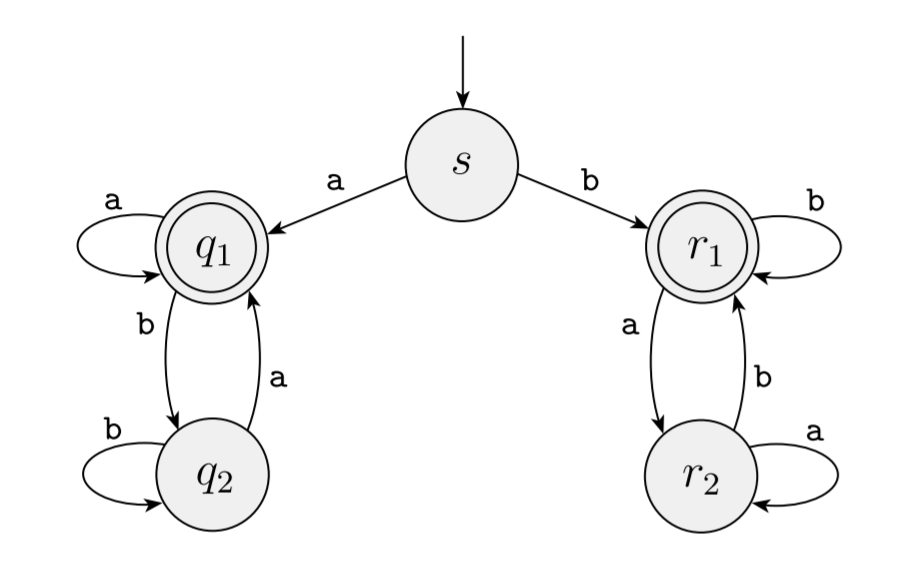
\includegraphics[scale=0.4]{assets/finite_automaton_3.png}
\end{center}
Here, the formal description of $M_3$ is as follows: 
\[M_3 = (\{s, q_1, q_2, r_1, r_2\}, \{\code{a, b}\}, \delta, s, \{q_1, r_1\})\]
Where $\delta$ is: 
\begin{center}
    \begin{tabular}{c|c c}
            & \code{a} & \code{b} \\
        \hline  
        $s$  & $q_1$ & $r_1$ \\ 
        $q_1$ & $q_1$ & $q_2$ \\ 
        $q_2$ & $q_1$ & $q_2$ \\ 
        $r_1$ & $r_2$ & $r_1$ \\ 
        $r_2$ & $r_2$ & $r_1$ \\
    \end{tabular}
\end{center}
Here, we note that we cannot end at the start state. In other words, when we start with \code{a}, we take the left branch to $q_1$. In the left branch, notice how when we end with \code{a}, we will always end up at $q_1$, the accept state. So, it follows that a string like the one below is acceptable: 
\[\code{a}w_2 w_3 \dots w_{n - 1} \code{a} \qquad w_i \in \{\code{a, b}\}\]
Likewise, if we start with \code{b}, we take the right branch to $r_1$. In the right branch, if our string ends with \code{b}, we will always end up at $r_1$. So, it follows that a string like the one below is also acceptable:
\[\code{b}w_2 w_3 \dots w_{n - 1} \code{b} \qquad w_i \in \{\code{a, b}\}\]
In other words, for this automaton, a string that starts and ends with the same symbol is accepted. That is: 
\[A = \{w \mid w \text{ starts and ends with the same symbol.}\}\]

\subsubsection{Example 3: Complicated Finite Automaton}
Sometimes, it is hard to describe a finite automaton by state diagram. In this case, we may end up using a formal description to specify the machine. Consider the following example with the alphabet: 
\[\Sigma = \{\code{RESET, 0, 1, 2}\}\]
Where \code{RESET} is treated as one symbol. For each $i \geq 1$, define $A_i$ to be the language of all strings where the sum of the numbers is a multiple of $i$, except that the sum is reset to 0 whenever the symbol \code{RESET} appears. For each $A_i$, we have a finite automaton $B_i$ which recognizes $A_i$. We define $B_i$ formally like so: 
\[B_i = (Q_i, \Sigma, \delta_i, q_0, \{q_0\})\]
Where $Q_i = \{q_0, q_1, q_2, \dots, q_{i - 1}\}$ and the transition function $\delta_i$ is defined so that for each $j$, if $B_i$ is in $q_j$ (i.e. $B_i$ is in state $q_j$), the running sum is $j$ modulo $i$. In other words, for each $q_j$ define: 
\[\delta_{i}(q_j, \code{0}) = q_j\]
\[\delta_{i}(q_j, \code{1}) = q_k \text{  where } k = j + 1 \text{ modulo } i\]
\[\delta_{i}(q_j, \code{2}) = q_k \text{  where } k = j + 2 \text{ modulo } i\]
\[\delta_{i}(q_j, \code{RESET}) = q_0\]

\bigskip

For example, suppose we have the following state machine $B_3$ which uses the same alphabet described above:
\begin{center}
    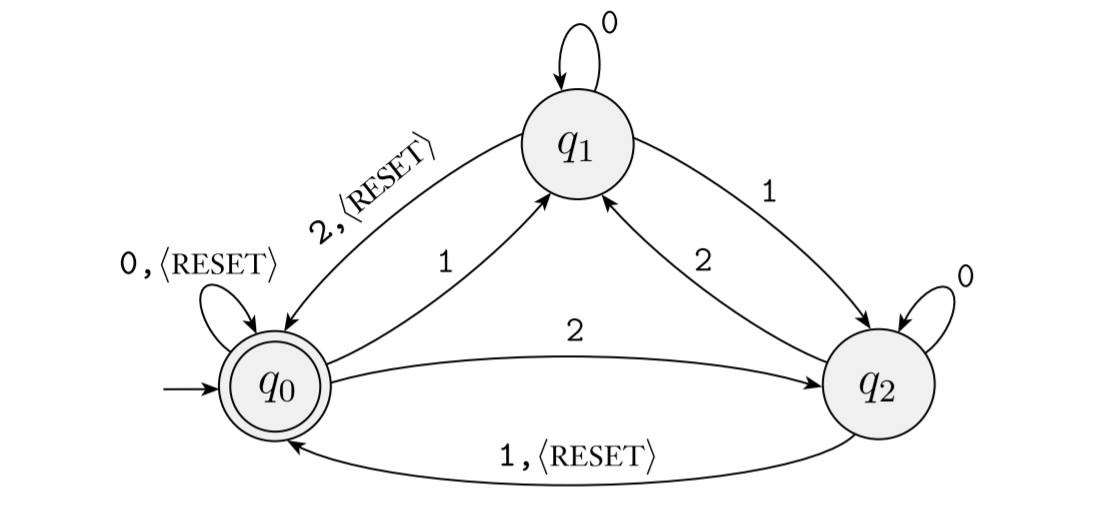
\includegraphics[scale=0.4]{assets/finite_automaton_4.png}
\end{center}
The formal description of $B_3$ is as follows: 
\[B_3 = (\{q_0, q_1, q_2\}, \{\code{RESET, 0, 1, 2}\}, \delta, q_0, \{q_0\})\]
Where $\delta$ is defined by: 
\begin{center}
    \begin{tabular}{c|c c c c}
              & \code{RESET} & \code{0} & \code{1} & \code{2} \\
        \hline  
        $q_0$ & $q_0$        & $q_0$    & $q_1$    & $q_2$    \\ 
        $q_1$ & $q_0$        & $q_1$    & $q_2$    & $q_0$    \\
        $q_2$ & $q_0$        & $q_2$    & $q_0$    & $q_1$
    \end{tabular}
\end{center}
So, as an example, let's suppose we have the string \code{01212}. The sum of these numbers is:
\[0 + 1 + 2 + 1 + 2 = 6 \implies 6 \equiv \boxed{0} \mod{3}\]
We expect the automaton to finish at the accept state as 6 is a multiple of 3. Running through the automaton, we have: 
\begin{itemize}
    \item Input: \code{0}. Start at $q_0$, end at $q_0$.
    \item Input: \code{1}. Start at $q_0$, end at $q_1$. So, our automaton is at state $q_1$.
    \item Input: \code{2}. Start at $q_1$, end at $q_0$. So, our automaton is at state $q_0$.
    \item Input: \code{1}. Start at $q_0$, end at $q_1$. So, our automaton is at state $q_1$.
    \item Input: \code{2}. Start at $q_1$, end at $q_0$. So, our automaton is at state $q_0$.
\end{itemize}
Therefore, we are at an accept state as our string \code{01212} sums up to a multiple of 3. Of course, if there are any \code{RESET}s in our string, we can disregard everything up to and including the \emph{last} \code{RESET} as \code{RESET} puts us back at the start. That is, for instance, the string \code{0121 RESET 21011 RESET 01212} will put the state machine in the same state as \code{01212}.

\bigskip

So, it follows that our state machine recognizes the set $A_3$, which consists of all strings where all digits sum up to 0 modulo 3. That is: 
\[A_3 = \left\{w \mid \sum_{\code{d} \in w} d = 0 \Mod{3}\right\}\]
\emph{Note:} If any \code{RESET}s are in the string, we can omit everything in the string \emph{up to and including} the last \code{RESET}.



\subsection{Formal Definition of Computation}
To review, let $M = (Q, \Sigma, \delta, q_0, F)$ be a finite automaton and let $w = w_1 w_2 \dots w_n$ be a string where each $w_i \in \Sigma$. Then, we say that $M$ accepts $w$ if a sequence of states $r_0, r_1, \dots, r_n$ in $Q$ exists with three conditions: 
\begin{enumerate}
    \item $r_0 = q_0$: The machine starts in the start state. 
    \item $\delta(r_i, w_{i + 1}) = r_{i + 1}$, for $i = 0, \dots, n - 1$: The machine goes from state to state according to the transition function. 
    \item $r_n \in F$: The machine accepts its input if it ends up in an accept state. 
\end{enumerate}
In particular, we say that $M$ recognizes language $A$ if $A = \{w \mid M \text{ accepts } w\}$.
\begin{definition}{Regular Language}{}
    A language is called a \textbf{regular language} if some finite automaton recognizes it.
\end{definition}

\subsubsection{Example 1: State Machine}
Recall, for example, our state machine $B_3$ in the previous lecture notes. If $w$ was the string:
\begin{verbatim}
    10 RESET 22 RESET 012
\end{verbatim}
Then, $M_5$ accepts $w$ according to the formal definition of computation because the sequence of states it enters when computing on $w$ is: 
\[q_0, q_1, q_1, q_0, q_2, q_1, q_0, q_0, q_1, q_0\]
In particular:
\begin{enumerate}
    \item The machine starts in the start state as expected. 
    \item The machine goes from state to state as expected. 
    \item The machine ends at the accept state. 
\end{enumerate}

\subsection{Designing Finite Automata}
A helpful approach when designing various types of automata is: 
\begin{mdframed}[]
    \emph{Put yourself in the place of the machine you are trying to design and then see how you would go about performing the machine's task.}
\end{mdframed} 
Suppose you are given some language and want to design a finite automaton that recognizes it. Given some input string, your goal is to determine if it is a member of the language the automaton is supposed to recognize. However, you can only see each symbol one at a time; after each symbol, you need to decide whether the string seen is in the language. The hardest part is that you need to figure out what you need to remember about the string as you are reading it. Remember: you only have a finite number of states, which means finite memory (hence, \emph{finite} automata). 

\subsubsection{Example 1: Designing a Finite Automaton}
Given $\Sigma = \{\code{0, 1}\}$, suppose we need to create a finite automaton $E_2$ that recognizes the regular language of all strings that contain \code{001} as a substring. For example, \code{001}, \code{1001}, \code{0010}, \code{111111001111101} are all in the language; however, \code{0000} and \code{11} are not.

\bigskip

Well, the first thing we can do is create the set of states that will result in an \code{ACCEPT} state. This is as simple as:
\begin{center}
    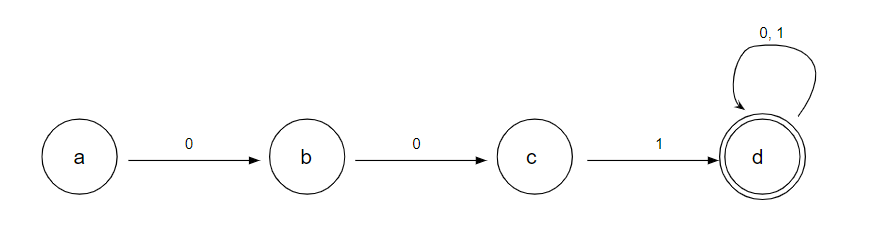
\includegraphics[scale=0.6]{assets/state_1.png}
\end{center}
Here, it's clear that a string like \code{001} will result in an \code{ACCEPT} state. Now, we need to account for any other strings. In particular, we need to account for several different possibilities:
\begin{itemize}
    \item We haven't seen any symbols associated with the pattern (e.g. we start with \code{1}s, or we saw a \code{0} and then a \code{1}). 
    \item We just saw \code{0}.
    \item We just saw \code{00}.
    \item We have seen the pattern \code{001}.
\end{itemize}
This gives us the automaton:
\begin{center}
    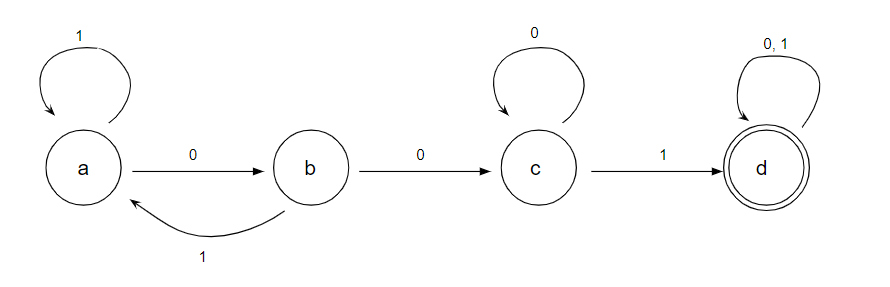
\includegraphics[scale=0.6]{assets/state_2.png}
\end{center}

\subsection{The Regular Operations}
In arithmetic, the basic objects are numbers and the tools are operations for manipulating them (e.g. $+$ or $\times$). In the theory of computation, the objects are languages and the tools include operations designed for manipulating them. We call these \textbf{regular operations}.

\begin{definition}{}{}
    Let $A$ and $B$ be languages. We define the regular operations \textbf{union}, \textbf{concatenation}, and \textbf{star} as follows: 
    \begin{itemize}
        \item \textbf{Union:} $A \cup B = \{x \mid x \in A \text{ or } x \in B\}$.
        \item \textbf{Concatenation:} $A \circ B = \{xy \mid x \in A \text{ and } y \in B\}$
        \item \textbf{Star:} $A^* = \{x_1 x_2 \dots x_k \mid k \geq 0 \text{ and each } x_i \in A\}$
    \end{itemize}
\end{definition}
\textbf{Remarks:}
\begin{itemize}
    \item The union operation simply takes all strings in both $A$ and $B$ and puts them together into one language.
    \item The concatenation operation attaches a string from $A$ in front of a string from $B$ in \emph{all possible ways to get the strings in the new language}.
    \item The star operation attaches any number of strings in $A$ together to get a string in the new language. Note that \emph{any number} includes 0, so the empty string $\epsilon$ is always in $A^*$.
\end{itemize}

\subsubsection{Example 1: String Manipulation}
Suppose $\Sigma = \{\code{a, b, ..., z}\}$ is the standard 26 letters. Define the two languages to be:
\[A = \{\code{good, bad}\}\]
\[B = \{\code{boy, girl}\}\]
Then: 
\begin{itemize}
    \item $A \cup B = \{\code{good, bad, boy, girl}\}$
    \item $A \circ B = \{\code{goodboy, goodgirl, badboy, badgirl}\}$
    \item $A^* = \{\epsilon, \code{good, bad, goodgood, goodbad, badgood, badbad, goodgoodgood, ...}\}$
\end{itemize}

\subsection{Justifying DFAs}
To prove that the DFA that we build, $M$, actually recognizes the language $L$, we ask the following questions: 
\begin{enumerate}
    \item Is every string accepted by $M$ in $L$?
    \item Is every string from $L$ accepted by $M$?\footnote{The contrapositive version is: Is every string rejected by $M$ not in $L$?}
\end{enumerate}
A string is accepted by a DFA when: 
\[ L(M) = \{ w \mid \delta^{*}(q_0, w) \in F \} \]
Where $\delta^*$ is defined by: 
\[\delta^{*}(q, w) = \begin{cases}
    q & w = \epsilon \\ 
    \delta(q, c) & w = c, c \in \Sigma \\ 
    \delta^{*}(\delta(q, c), w') & w \subset w', c \in \Sigma, w' \in \Sigma^*
\end{cases}\]


\subsection{Complementation of DFAs}
\begin{theorem}{Complementation}{}
    If $A$ is a regular language over $\{0, 1\}^*$, then so is its complement. 
\end{theorem}
\textbf{Remarks:}
\begin{itemize}
    \item This is essentially the same thing as saying that the class of regular languages is closed under complementation.
    \item How do we apply this? Let $A$ be a regular language. Then, there is a DFA $M = (Q, \Sigma, \delta, q_0, F)$ such that $L(M) = A$. We want to build a DFA $M'$ whose language is $\overline{A}$. Define: 
    \[M' = (Q, \Sigma, \delta, q_0, Q \setminus F)\]
\end{itemize}

\begin{proposition}
    $M'$ accepts $A^c$.
\end{proposition}

\begin{mdframed}[]
    \begin{proof}
        Because $M$ accepts $A$, we define $A$ to be: 
        \[A = \{w \mid M \text{ accepts } w\} = \{w \mid \delta^{*}(q_0, w) \in F\}\]
        Recall that $\delta^{*}(q, w)$ is the state reached from $q$ after reading the word $w$. Taking the complement of $A$, we have: 
        \[A^c = \{w \mid w \notin A\} = \{w \mid \delta^{*}(q_0, w) \notin F\} = \{w \mid \delta^{*}(q_0, w) \in Q \setminus F\}\]
        So, $M'$ accepts $A^c$. 
    \end{proof}
\end{mdframed}

\subsubsection{Example 1: Building DFA}
Construct a DFA that recognizes $\{w \mid w \text{ contains the substring baba}\}$.

\begin{mdframed}[nobreak=true]
    \begin{center}
        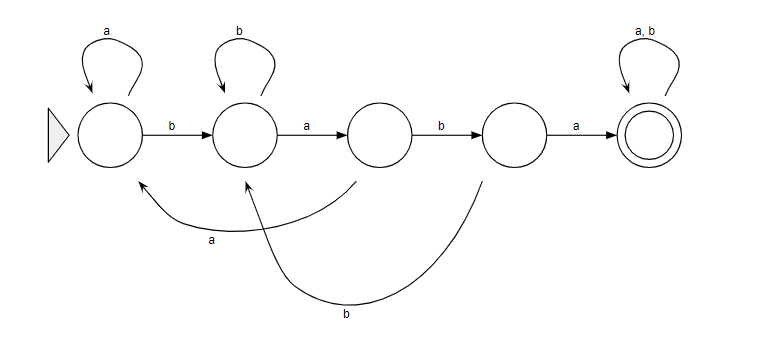
\includegraphics[scale=0.7]{assets/baba_state.png}
    \end{center}
\end{mdframed}

\subsubsection{Example 2: Building DFA}
Construct a DFA that recognizes $\{w \mid w \text{ doesn't contain the substring baba}\}$.

\begin{mdframed}[nobreak=true]
    \begin{center}
        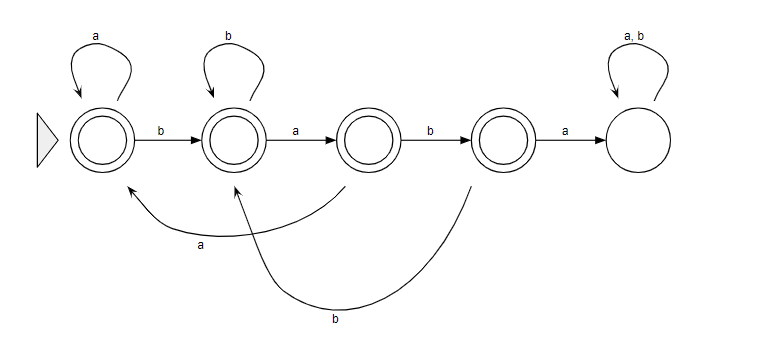
\includegraphics[scale=0.7]{assets/not_baba_state.png}
    \end{center}
\end{mdframed}

\subsection{Regular Operations}
In arithmetic, the basic objects are numbers and the tools are operations for manipulating them (e.g. $+$ or $\times$). In the theory of computation, the objects are languages and the tools include operations designed for manipulating them. We call these \textbf{regular operations}.

\begin{definition}{}{}
    Let $A$ and $B$ be languages. We define the regular operations \textbf{union}, \textbf{concatenation}, and \textbf{star} as follows: 
    \begin{itemize}
        \item \textbf{Union:} $A \cup B = \{x \mid x \in A \text{ or } x \in B\}$.
        \item \textbf{Concatenation:} $A \circ B = \{xy \mid x \in A \text{ and } y \in B\}$
        \item \textbf{(Kleene) Star:} $A^* = \{x_1 x_2 \dots x_k \mid k \geq 0 \text{ and each } x_i \in A\}$
    \end{itemize}
\end{definition}
\textbf{Remarks:}
\begin{itemize}
    \item The union operation simply takes all strings in both $A$ and $B$ and puts them together into one language.
    \item The concatenation operation attaches a string from $A$ in front of a string from $B$ in \emph{all possible ways to get the strings in the new language}.
    \item The star operation attaches any number of strings in $A$ together to get a string in the new language. Note that \emph{any number} includes 0, so the empty string $\epsilon$ is always in $A^*$.
\end{itemize}
Note that we can prove the union operation today, but we cannot prove the concatenation or star operators until later.

\subsubsection{Union}
\begin{theorem}{}{}
    The class of regular languages over a fixed alphabet $\Sigma$ is closed under the union operator. 
\end{theorem}
\textbf{Remark:} In other words, if $A_1$ and $A_2$ are regular language, so is $A_1 \cup A_2$.

\bigskip 

Essentially, we want to show that if we have two regular languages $A$ and $B$, then the union of them must also be regular. Thus, we want to show that if $M_1$ is the DFA for $A$ and $M_2$ is the DFA for $B$, then there is a DFA that recognizes $A \cup B$:
\begin{itemize}
    \item The goal is to build a DFA that recognizes $A \cup B$. 
    \item The strategy is to use DFAs that recognize each of $A$ and $B$. 
\end{itemize}
A basic sketch of this proof is as follows: 
\begin{mdframed}[]
    \begin{proof}
        We want to show that $M$ accepts $w$ if $M_1$ accepts $w$ \emph{or} $M_2$ accepts $w$. Let $A$ and $B$ be any two regular languages over $\Sigma$. Given:
        \[M_1 = (Q_1, \Sigma, \delta_1, q_1, F_1) \qquad L(M_1) = A\]
        \[M_2 = (Q_2, \Sigma, \delta_2, q_2, F_2) \qquad L(M_2) = B\]
        We want to show that $A \cup B$ is regular. The idea is to run these two DFAs $M_1$ and $M_2$ in parallel. So, we define: 
        \[M = (Q_1 \times Q_2, \Sigma, \delta, (q_1, q_2), F)\]
        Where, for $r \in Q_1$, $s \in Q_2$, and $x \in \Sigma$, we define:
        \[\delta((r, s), x) = (\delta_{1}(r, x), \delta_{2}(s, x))\]
        \[F = \{(r, s) \mid r \in F_1 \text{ or } s \in F_2\}\]
        \begin{mdframed}[]
            Note that it is not $\{(r, s) \mid r \in F_1 \text{ and } s \in F_2\}$ because this would be under intersection. Likewise, it is not $F_1 \times F_2$ because it is also intersection. 
        \end{mdframed}

        (And so on...)
    \end{proof}
\end{mdframed}

\subsubsection{Intersection}
\begin{mdframed}[]
    \begin{proof}
        The proof is left for another day.
    \end{proof}
\end{mdframed}

\begin{theorem}{}{}
    The class of regular languages is closed under the concatenation operation.
\end{theorem}
\textbf{Remark:} In other words, if $A_1$ and $A_2$ are regular language, then so is $A_1 \circ A_2$.

\bigskip 

How would you prove that the class of regular languages is closed under intersection? The idea is that:
\[A \cap B = (A^c \cup B^c)^c\]
We've already shown that the union is closed and so is its complement. 

\subsubsection{Payoff}
Consider the set: 
\[
    \{w \mid w \text{ contains neither the substrings aba nor baab}\}  
\]
Is this a regular set? 

\begin{mdframed}[]
    We know that:
    \[A = \{w \mid w \text{ contains aba as a substring}\}\]
    \[B = \{w \mid w \text{ contains baab as a substring}\}\]
    From which we know: 
    \[\overline{A} \cap \overline{B} = \overline{A \cup B}\]
\end{mdframed}









































\newpage 
\section{Nondeterministic Finite Automata (1.2)}
In a deterministic finite automata, when the machine was in a given state and reads the next input symbol, we knew that the next state is; that's why it's called \emph{determinstic}, because it was already determined. \textbf{However}, in a \emph{nondeterministic} machine, several choices may exist for the next state at any point. In general, nondeterminism is a \emph{generalization} of determinism; that is, every deterministic finite automaton is automatically a nondeterminism finite automaton.

\subsection{The Differences Between DFA and NFA}
\begin{center}
    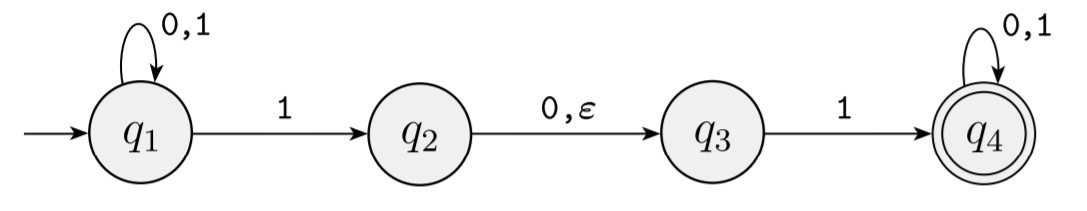
\includegraphics[scale=0.4]{assets/nfa_1.png}
    
    \textbf{Figure:} The nondeterministic finite automaton $N_1$. 
\end{center}

\begin{center}
    \begin{tabular}{p{3in}|p{3in}}
        \textbf{DFA} & \textbf{NFA} \\ 
        \hline 
        \begin{itemize}
            \item Every state of a DFA always has exactly one exiting transition arrow for each symbol in the alphabet.
            \item There is a unique computation path for each input. 
            \item Labels on the transition arrows are symbols from the alphabet. 
        \end{itemize} 

        & \begin{itemize}
            \item Not every state in an NFA needs exactly one transition arrow for each symbol. In an NFA, a state may have zero, one, or many exiting arrows for each alphabet symbol.
            \item We may allow several (or zero) alternative computations on the same input. 
            \item NFAs may have arrows labeled with members of the alphabet or $\epsilon$. Zero, one, or many arrows may exit from each state with the label $\epsilon$. For example, the above figure has one transition arrow with $\epsilon$ as a label. 
        \end{itemize}
    \end{tabular}
\end{center}

\subsection{NFA Computation}
How does an NFA compute? Suppose that we are running an NFA on an input string and come to a state with multiple ways to proceed. Suppose, in fact, that we use the NFA above: $N_1$. Additionally, suppose that we are at state $q_1$, and the next input symbol is \code{1}. 
\begin{itemize}
    \item After reading this symbol, the machine \textbf{splits into multiple copies of itself} and follows \emph{all} the possibilities in \emph{parallel}. In other words, each copy of the machine takes one of the possible ways to proceed and continues as before. 
    \item If there are subsequent choices, the machine splits again. 
    \item If the next input symbol doesn't appear on any of the arrows exiting the stae occupied by a copy of the machine, that copy of the machine dies.
    \item If any one of these copies of the machine is in an accept state at the \underline{end of the input}, the NFA \emph{accepts} the input string.
\end{itemize}
What happens when we come across a state with an $\epsilon$ symbol on an exiting arrow? Well, without reading any input, the machine splits into \emph{multiple} copies, one following each of the exiting $\epsilon$-labeled arrows and one staying at the current state. The machine, then, proceeds nondeterministically as before. So, really, $\epsilon$ transitions allow the machine to \textbf{transition between states spontaneously} without consuming any input symbols.

\begin{center}
    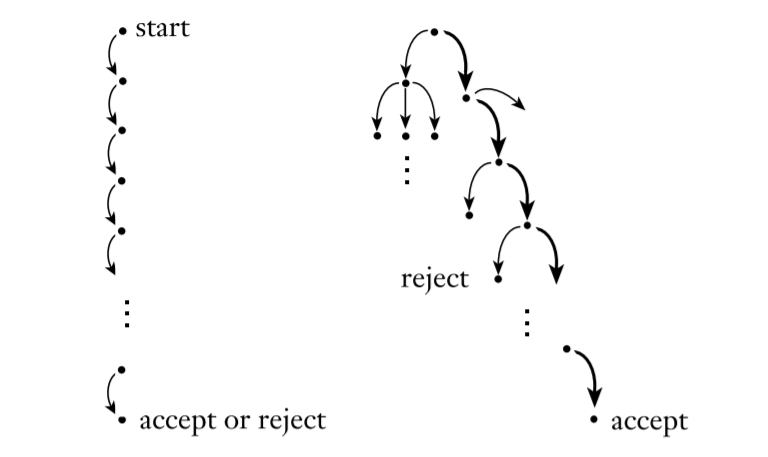
\includegraphics[scale=0.4]{assets/nfa_vs_dfa.png}

    \textbf{Figure:} Difference between deterministic computation and nondeterministic computation. 
\end{center}

We can see nondeterminism as some kind of parallel computation, where multiple independent ``threads'' or ``processes'' can be started concurrently. Whenever the NFA splits to follow several choices, that corresponds to a process ``forking'' into several children, of which each proceeds separately. Also, if one of the processes accepts, the entire computation accepts. 


\subsection{Formal Definition of NFA}
The formal definition of a nondeterministic finitne automaton is essentially the same as the one for a deterministic finitne automaton. The major difference, though, is the transition function. In particular:
\begin{center}
    \begin{tabular}{p{3in}|p{3in}}
        \textbf{DFA} & \textbf{NFA} \\ 
        \hline 
        The transition function takes a state and an input symbol, and produces the next state. & The transition function takes a state and an input symbol \emph{or} the empty string, and produces the \emph{set of possible next states}.
    \end{tabular}
\end{center}

With this in mind, we consider the definition:
\begin{definition}{Nondeterministic Finite Automaton}{}
    A \textbf{nondeterministic finite automaton} is a 5-tuple $(Q, \Sigma, \delta, q_0, F)$ where: 
    \begin{enumerate}
        \item $Q$ is a finite set called the \textbf{states}.
        \item $\Sigma$ is a finite set called the \textbf{alphabet}.
        \item $\delta: Q \times \Sigma \cup \{\epsilon\} \mapsto \PowerSet(Q)$ is the \textbf{transition function}.
        \item $q_0 \in Q$ is the \textbf{start state}.
        \item $F \subseteq Q$ is the \textbf{set of accept states} (sometimes also called \emph{final states}).
    \end{enumerate}
\end{definition}
\textbf{Remarks:}
\begin{itemize}
    \item $\Sigma \cup \{\epsilon\}$ is sometimes written as $\Sigma_{\epsilon}$.
    \item We say that $\delta(q, c)$ returns a \textbf{set} of states; more precisely, a subset of $Q$. Here, $c \in \Sigma$ or $\epsilon$ and $q \in Q$.
\end{itemize}

\subsubsection{Example: Starting NFA}
Recall the NFA $N_1$:
\begin{center}
    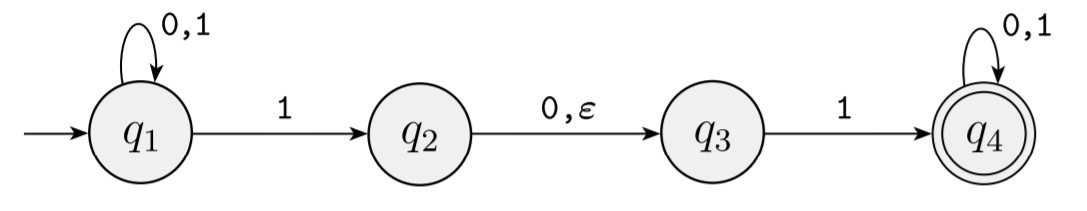
\includegraphics[scale=0.4]{assets/nfa_1.png}
\end{center}
Here, the formal description of $N_1$ is given by: 
\begin{itemize}
    \item $Q = \{q_1, q_2, q_3, q_4\}$
    \item $\Sigma = \{\code{0}, \code{1}\}$
    \item $\delta$ is given as:
    \begin{center}
        \begin{tabular}{c|c c c}
                  & \code{0} & \code{1} & $\epsilon$ \\ 
            \hline 
            $q_1$ & $\{q_1\}$ & $\{q_1, q_2\}$ & $\emptyset$ \\ 
            $q_2$ & $\{q_3\}$ & $\emptyset$ & $\{q_3\}$ \\ 
            $q_3$ & $\emptyset$ & $\{q_4\}$ & $\emptyset$ \\ 
            $q_4$ & $\{q_4\}$ & $\{q_4\}$ & $\emptyset$
        \end{tabular}
    \end{center}
    \item $q_1$ is the start state
    \item $F = \{q_4\}$
\end{itemize}

\subsection{Acceptance in an NFA}
We say that an NFA $(Q, \Sigma, \delta, q_0, F)$ accepts a string $w$ in $\Sigma^*$ if and only if we can write $w = y_1 y_2 \dots y_m$ where each $y_i \in \Sigma_{\epsilon}$ and there is a sequence of states $r_0, \dots, r_m \in Q$ such that: 
\begin{enumerate}
    \item $r_0 = q_0$. The machine starts in the start state. 
    \item $r_{i + 1} \in \delta(r_i, y_{i + 1})$ for each $i = 0, 1, \dots, m - 1$. The state $r_{i + 1}$ is one of the allowable next states when $N$ is in state $r_i$ and reading $y_{i + 1}$. Here, we note that $\delta(r_i, y_{i + 1})$ is the set of allowable next states.  
    \item $r_m \in F$. The machine accepts its input if the last state is an accept state. 
\end{enumerate}



\subsection{Equivalence of NFAs and DFAs}
Deterministic and nondeterministic finite automata both recognize the same class of languages.

\begin{theorem}{}{}
    Every nondeterministic finite automaton has an equivalent deterministic finite automaton.
\end{theorem}
\textbf{Remark:} Here, we say that two machines are equivalent if they recognize the same language. 

\bigskip 

The proof is as follows\footnote{This proof was used in our submission for HW2 Problem 3 (CSE 105, WI22). The group members involved in this submission are (only initials and the last two digits of their PID are shown): CB (67), TT (96), ASRJ (73), and me.}:
\begin{mdframed}[]
    \begin{proof}
        Let $N = (Q, \Sigma, \delta, q_0, F)$ be the NFA that recognizes the language $L$. We want to show that there is a DFA $M = (Q', \Sigma, \delta', q_0', F')$ which recognizes the same $L$. 
        \begin{enumerate}
            \item First, $Q' = \mathcal{P}(Q)$. This is because must have the states in $Q'$ to represents the possible subset of states in $Q$. In an NFA, we can make multiple copies of the automaton, which may end up at different states over time. We therefore need to account for where these copies can be in our corresponding DFA. 
 
            \item The alphabet $\Sigma$ is the same in both the NFA and DFA. 
 
            \item The transition function of the corresponding DFA is defined by: 
            \[\delta'(X, x) = \{q \in Q \mid q \in \delta(r, x) \text{ for some } r \in X \text{ or accessible via } \epsilon \text{ transitions}\}\]
            Where $X$ is a state of the DFA and $x \in \Sigma$. Because a state in an NFA can have multiple outgoing transition arrows under the same type (e.g. two outgoing arrows for \texttt{a}), we need to account for this in the corresponding NFA. This is our first condition in our $\delta'$ function; in this sense, if we consider the possible states that we can go to in the NFA, then the corresponding state in our DFA is the union of all of those possible states. 
            We must also consider that, for a given state in an NFA, there may be $\epsilon$ transitions. In case there are $\epsilon$ transitions, we need to consider where the $\epsilon$ transitions put a copy of the machine.

            \item The start state in the corresponding DFA is the set $q_0' = \{q_0\} \cup \delta^{*} (q_0, \epsilon)$. First, we note that the start state in the NFA is $q_0$; thus, the start state in the corresponding DFA must be \emph{at least} $\{q_0\}$. However, if there are any $\epsilon$ transitions from the start state, we must consider those as well since transitioning to another state from the state state via the $\epsilon$ transition doesn't consume any input. 

            \item The set of final states in the corresponding DFA is simply:
            \[F' = \{X \mid X \subseteq Q \text{ and } X \cap F \neq \emptyset\}\]
            Here, we're saying that if there are any sets in $Q'$ which contain a final state in $F$, then said set must be a final set. This is because, in a NFA, we may have multiple copies of the machine running, and if one copy stops at a final state, then the NFA is accepted (despite the other copies not necessarily being at a final state).
        \end{enumerate}
        The rest of the proof is omitted for now. 
    \end{proof}
\end{mdframed}

\subsubsection{Example: NFA to DFA}
Consider the following NFA $N$:
\begin{center}
    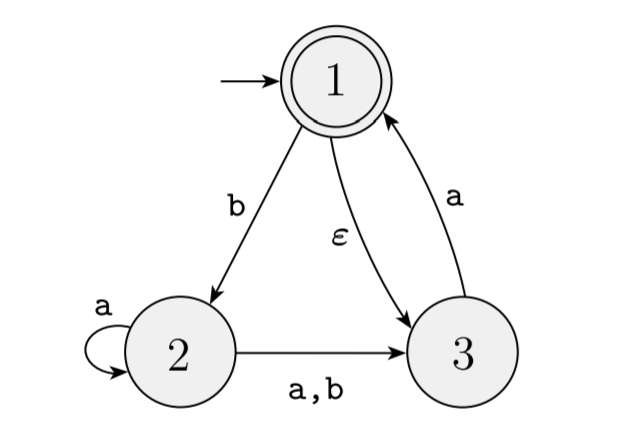
\includegraphics[scale=0.5]{assets/nfa_to_dfa_1.png}

    \textbf{Figure:} The NFA $N$. 
\end{center}
We can define $N = (Q, \Sigma, \delta, q_0, F)$ like so: 
\begin{itemize}
    \item $Q = \{\code{1}, \code{2}, \code{3}\}$
    \item $\Sigma = \{\code{a}, \code{b}\}$
    \item $\delta$ is defined by 
    \begin{center}
        \begin{tabular}{c|c c c}
                & \code{a} & \code{b} & $\epsilon$ \\ 
            \hline 
            1   & $\emptyset$ & $\{2\}$ & $\{3\}$ \\ 
            2   & $\{2, 3\}$ & $\{3\}$ & $\emptyset$ \\ 
            3   & $\{1\}$ & $\emptyset$ & $\emptyset$
        \end{tabular}
    \end{center}
    \item $q_0 = 1$
    \item $F = \{1\}$
\end{itemize}
We're now being asked to construct a corresponding DFA: 
\[D = (Q', \Sigma', \delta', q_0', F')\]
Here, it's trivial to note that: 
\begin{itemize}
    \item $Q' = \PowerSet(Q) = \{\emptyset, \{1\}, \{2\}, \{3\}, \{1, 2\}, \{1, 3\}, \{2, 3\}, \{1, 2, 3\}\}$. 
    \item $\Sigma = \{\code{a}, \code{b}\}$
    \item $q_0 = \{1, 3\}$. This is because we can start at both state 1 and 3 since 3 has an $\epsilon$ transition.
    \item $F' = \{\{1\}, \{1, 2\}, \{1, 3\}, \{1, 2, 3\}\}$. This is because we want all subsets that contain $N$'s accept state. 
\end{itemize}
The hard part is actually ``wiring'' the DFA up, i.e. the transition function. To do this, we need to analyze how the NFA acts and ``translate'' it to what the DFA would do. So, let's consider each element in $Q'$ and see how it would relate to the NFA. 
\begin{itemize}
    \item Consider $\{1\} \in Q'$. In the NFA:
    \begin{itemize}
        \item $1$ doesn't go anywhere when \code{a} is given by itself. \textbf{However}, $1$ can go to $3$ since this is an $\epsilon$ transition, and $3$ goes to $1$ when consuming \code{a}, so it follows that $\boxed{\{1\} \xrightarrow{\code{a}} \{1, 3\}}$ in the corresponding DFA. 
        \item $1$ goes to $2$ when \code{b} is given, so it follows that $\boxed{\{1\} \xrightarrow[]{\code{b}} \{2\}}$ in the corresponding DFA. 
    \end{itemize}
    \item Consider $\{2\} \in Q'$. In the NFA: 
    \begin{itemize}
        \item $2$ goes to $2$ \emph{and} $3$ when \code{a} is given, so it follows that $\boxed{\{2\} \xrightarrow{\code{a}} \{2, 3\}}$ in the corresponding DFA. 
        \item $2$ goes to $3$ when \code{b} is given, so it follows that $\boxed{\{2\} \xrightarrow[]{\code{b}} \{3\}}$ in the corresponding DFA. 
    \end{itemize}
    \item Consider $\{3\} \in Q'$. In the NFA: 
    \begin{itemize}
        \item $3$ goes to $1$ when \code{a} is given, but then it can also go to $3$ since there is an $\epsilon$ transition, so it follows that $\boxed{\{3\} \xrightarrow{\code{a}} \{1, 3\}}$. 
        \item $3$ doesn't go anywhere when \code{b} is given, so it follows that $\boxed{\{3\} \xrightarrow{\code{b}} \emptyset}$.
    \end{itemize}
\end{itemize}
We can use the above to build cases for the remaining elements in $Q'$.
\begin{itemize}
    \item Consider $\{1, 2\} \in Q'$. In the corresponding NFA, this means that there's a copy at state $1$ and a copy at state $2$. So: 
    \begin{itemize}
        \item Suppose \code{a} is given. Then, from our previous work, we know that $\{1\} \xrightarrow{\code{a}} \{1, 3\}$, and $\{2\} \xrightarrow{\code{a}} \{2, 3\}$.
        Therefore, $\boxed{\{1, 2\} \xrightarrow{\code{a}} \{1, 2, 3\}}$ (recall that we take the union).
        \item Suppose \code{b} is given. Then, we know that $\{1\} \xrightarrow{\code{b}} \{2\}$, and $\{2\} \xrightarrow[]{\code{b}} \{3\}$. Therefore, $\boxed{\{1, 2\} \xrightarrow[]{\code{b}} \{2, 3\}}$. 
    \end{itemize}
    
    \item Consider $\{1, 3\} \in Q'$. In the corresponding NFA, this means that there's a copy at state $1$ and a copy at state $3$. So: 
    \begin{itemize}
        \item Suppose \code{a} is given. Then, from our previous work, we know that $\{1\} \xrightarrow{\code{a}} \{1, 3\}$, and $\{3\} \xrightarrow{\code{a}} \{1, 3\}$.
        Therefore, $\boxed{\{1, 3\} \xrightarrow{\code{a}} \{1, 3\}}$.
        \item Suppose \code{b} is given. Then, we know that $\{1\} \xrightarrow{\code{b}} \{2\}$, and $\{3\} \xrightarrow[]{\code{b}} \emptyset$. Therefore, $\boxed{\{1, 3\} \xrightarrow[]{\code{b}} \{2\}}$. 
    \end{itemize}
    
    \item Consider $\{2, 3\} \in Q'$. In the corresponding NFA, this means that there's a copy at state $2$ and a copy at state $3$. So: 
    \begin{itemize}
        \item Suppose \code{a} is given. Then, from our previous work, we know that $\{2\} \xrightarrow{\code{a}} \{2, 3\}$, and $\{3\} \xrightarrow{\code{a}} \{1, 3\}$.
        Therefore, $\boxed{\{2, 3\} \xrightarrow{\code{a}} \{1, 2, 3\}}$.
        \item Suppose \code{b} is given. Then, we know that $\{2\} \xrightarrow{\code{b}} \{3\}$, and $\{3\} \xrightarrow[]{\code{b}} \emptyset$. Therefore, $\boxed{\{2, 3\} \xrightarrow[]{\code{b}} \{3\}}$. 
    \end{itemize}

    \item Consider $\{1, 2, 3\} \in Q'$. In the corresponding NFA, this means that there's a copy at state $1$, $2$, and $3$. So: 
    \begin{itemize}
        \item Suppose \code{a} is given. From our previous work, we know that $\boxed{\{1, 2, 3\} \xrightarrow{\code{a}} \{1, 2, 3\}}$.
        \item Suppose \code{b} is given. From our previous work, we know that $\boxed{\{1, 2, 3\} \xrightarrow{\code{b}} \{2, 3\}}$.
    \end{itemize}
\end{itemize}

This gives us the following DFA: 
\begin{center}
    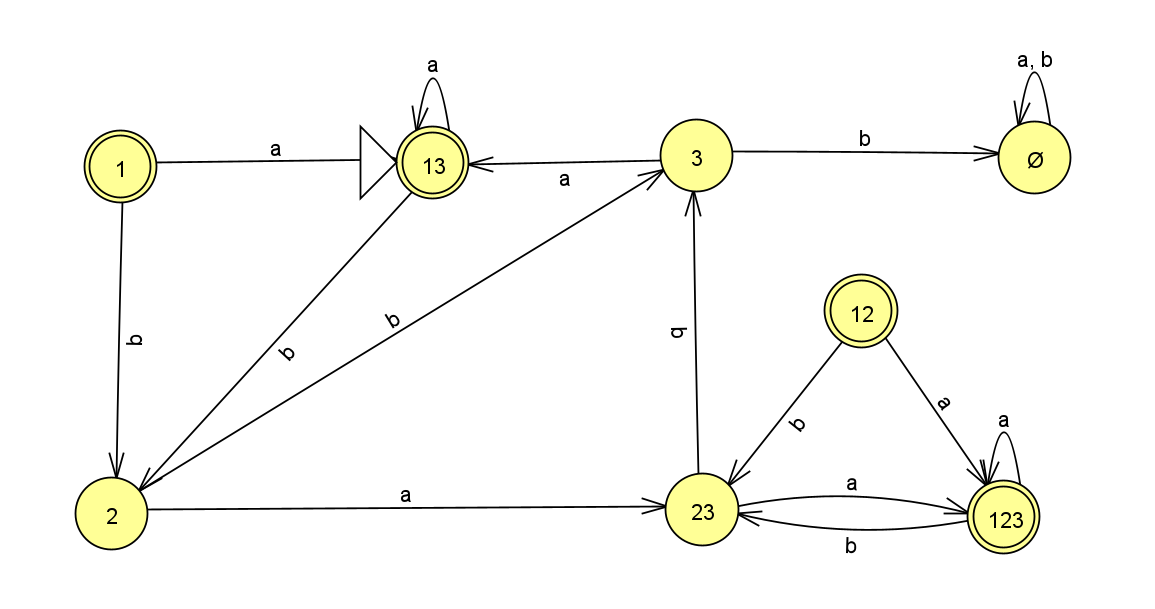
\includegraphics[scale=0.50]{assets/nfa_to_dfa_2.png}
\end{center}

However, we note a few things.
\begin{itemize}
    \item State $1$ doesn't have anything coming into it. Therefore, we can remove it.
    \item State $12$ doesn't have anything coming into it. Therefore, we can remove it.
\end{itemize}
This gives us the simplified DFA: 
\begin{center}
    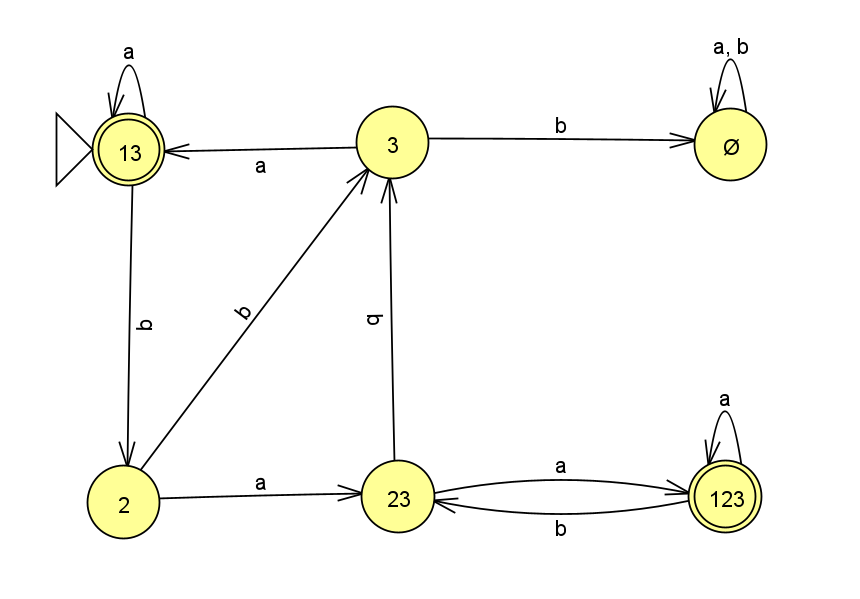
\includegraphics[scale=0.50]{assets/nfa_to_dfa_3.png}
\end{center}

\subsection{Applications of Theorem}
There are several applications of this theorem. 

\begin{corollary}{}{}
    A language is regular if and only if some nondeterministic finite automaton recognizes it.
\end{corollary}


\begin{theorem}{}{}
    The class of regular languages is closed under the union operation.
\end{theorem}

\begin{mdframed}[]
    \begin{proof}
        (Sketch.) Suppose $A_1$ and $A_2$ are regular languages. We want to show that $A_1 \cup A_2$ is regular. We can take two NFAs, $N_1$ for $A_1$ and $N_2$ for $A_2$, and combine them to make one new NFA $N$. The idea is that $N$ must accept its input if either $N_1$ and $N_2$ accepts. So, essentially, we want to run both $N_1$ and $N_2$ in parallel. To simulate this behavior, we can create a new start state $q_0$ with two $\epsilon$ transitions pointing to the original start states of $N_1$ and $N_2$ (everything else about $N_1$ and $N_2$ are left unchanged).    
    \end{proof}
\end{mdframed}

\begin{center}
    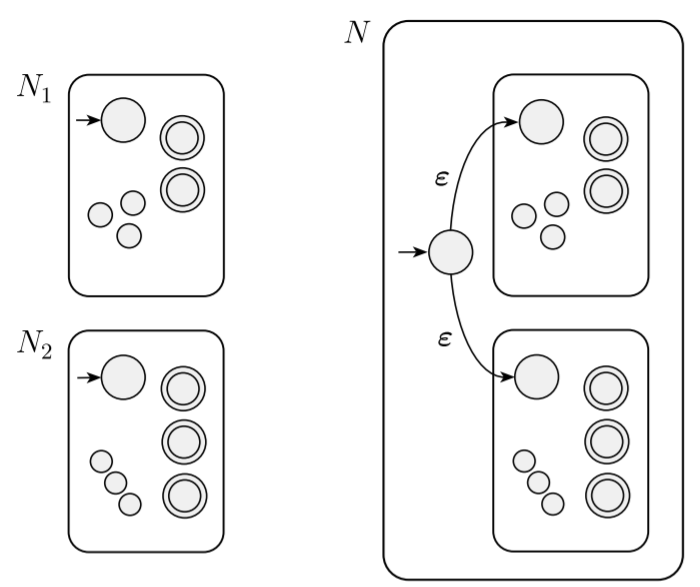
\includegraphics[scale=0.5]{assets/union_nfa.png}
\end{center}


\begin{theorem}{}{}
    The class of regular languages is closed under the concatenation operation.
\end{theorem}

\begin{mdframed}[]
    \begin{proof}
        (Sketch.) Suppose $A_1$ and $A_2$ are regular languages. We want to show that $A_1 \circ A_2$ is regular. We can take two NFAs, $N_1$ for $A_1$ and $N_2$ for $A_2$, and combine them to make one new NFA $N$. The idea for $N$ is as follows: 
        \begin{itemize}
            \item Start at the starting state for $N_1$ and remove the starting state for $N_2$. 
            \item Connect each accept state in $N_1$ to the original start state in $N_2$. The accept states in $N_1$ will no longer be accept states.  
        \end{itemize}
        By starting at the $N_1$ part of $N$, we guarantee that we will recognize some language $A_1$. Then, once we hit the original accept state in $N_1$, we can evaluate the rest of the string in $N_2$. If we hit an accept state in $N_2$, then we have recognized $A_1 \circ A_2$. 
    \end{proof}    
\end{mdframed}

\begin{center}
    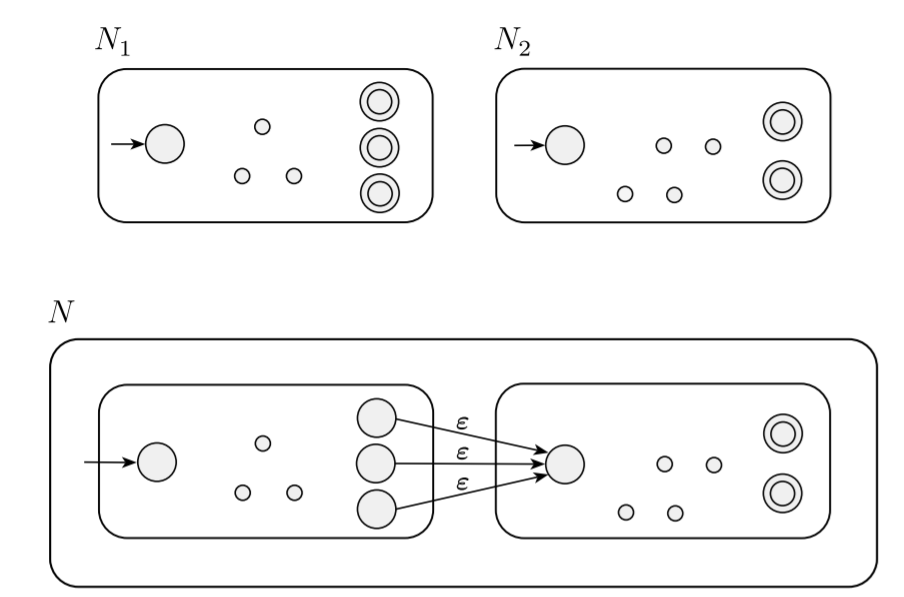
\includegraphics[scale=0.5]{assets/concat_nfa.png}
\end{center}


\begin{theorem}{}{}
    The class of regular languages is closed under the star operation.
\end{theorem}

\begin{mdframed}[]
    \begin{proof}
        (Sketch.) Suppose $A_1$ is a regular language. We want to show that $A_1^*$ is also regular. Consider the NFA $N_1$ for $A_1$. We want to modify $N_1$ so it recognizes $A_1^*$. Thus, our idea for the new NFA $N$ is as follows: 
        \begin{itemize}
            \item Because $\epsilon$ (the empty string) is valid under $A_1^*$, we must make a new start state that goes to the original start state; then, we can make the transition from the new start state to the original start state $\epsilon$. 
            \item We can connect the accept states in $N_1$ back to the original start state (not the new start state) with the labels being $\epsilon$.
            \item The accept states in $N_1$ is the same for $N$. 
        \end{itemize}
        By starting at the new start state, we can guarantee that $\epsilon$ will be accepted if it is the only thing to be read. Processing the string is as expected. However, once we reach the accept state, we need to \emph{go back} to the original start state to process the next ``word.'' This process keeps going until we no longer have any words to process. In this case, if we end off at any accept state with nothing left to read, then we accept. 
    \end{proof}
\end{mdframed}

\begin{center}
    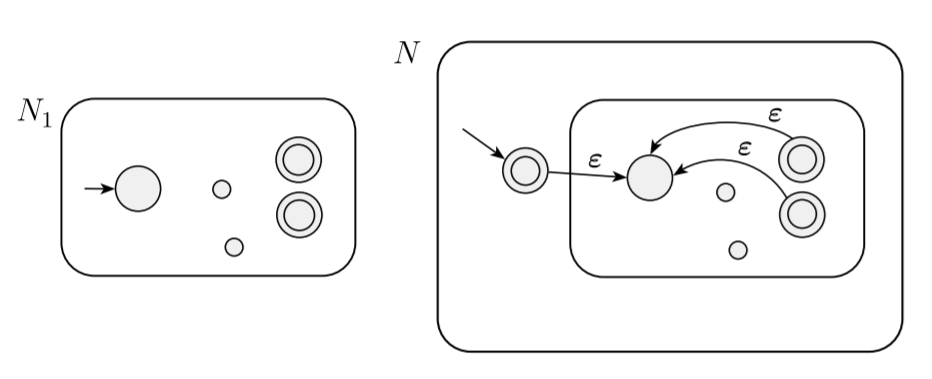
\includegraphics[scale=0.5]{assets/star_nfa.png}
\end{center}









































\newpage 
\section{Regular Expressions (1.3)}
We can use \textbf{regular expressions} (RegExp) to describe a language. An example of a regular expression is: 
\[(\code{0} \cup \code{1}) \code{0}^*\]
To give a comparison, consider the arithmetic expression:
\[(5 + 4) \times 2\]
In an arithmetic expression, the value is a number; in our case above, we would get 18. In a regular expression, the value is a \textbf{language}; in our case above, we can break the expression into multiple parts: 
\begin{itemize}
    \item $\code{0} \cup \code{1}$: This is the same thing as saying $\{\code{0}\} \cup \{\code{1}\}$, so this segment is saying that its language is $\{\code{0}, \code{1}\}$.
    \item $\code{0}^*$: This is the same thing as saying $\{\code{0}\}^*$, so its value is the language consisting of all strings containing any numbers of \code{0}s.
\end{itemize}
Putting it together, this regular expression recognizes any string which starts with \code{0} or \code{1} and ends with some number of \code{0}s. Just like how the multiplication sign $\times$ is often implicitly written (that is, we can write $2(5 + 4)$ instead of $2 \times (5 + 4)$), the concatenation sign $\circ$ is also implicitly written. That is, $(\code{0} \cup \code{1}) \code{0}^*$ is the shorthand for $(\code{0} \cup \code{1}) \circ \code{0}^*$. 

\subsection{Formal Definition of a Regular Expression}
\begin{definition}{Regular Expression}{}
    We say that $R$ is a \textbf{regular expression} if $R$ is: 
    \begin{enumerate}
        \item $a$ for some $a$ in the alphabet $\Sigma$,
        \item $\epsilon$,
        \item $\emptyset$,
        \item $(R_1 \cup R_2)$, where $R_1$ and $R_2$ are regular expressions,
        \item $(R_1 \circ R_2)$, where $R_1$ and $R_2$ are regular expressions,
        \item $(R_1^*)$, where $R_1$ is a regular expressions,
    \end{enumerate}
    In items 1 and 2, the regular expressions $a$ and $\epsilon$ represent the languages $\{a\}$ and $\{\epsilon\}$, respectively. In item 3, the regular expression $\emptyset$ represents the empty language. In items 4, 5, and 6, the expressions represent the languages obtained by taking the union or concatenation of the languages $R_1$ and $R_2$, or the star of the language $R_1$, respectively. 
\end{definition}
\textbf{Remarks:}
\begin{itemize}
    \item Remember, $\epsilon$ and $\emptyset$ are not the same. $\epsilon$ is the same thing as $\{\epsilon\}$, i.e. the language containing only the empty string; however, $\emptyset$ represents the language that doesn't contain anything. 
    \item In regular expressions, there is the notion of operator precedence. In our case, the star operation is done first, followed by concatenation, and finally union \emph{unless} parentheses change the usual order.
    \item We may omit the $\circ$ notation for concatenation. For example, $R_1 R_2$ is the same thing as $R_1 \circ R_2$.  
\end{itemize}
Additionally, we define some more notation.
\begin{itemize}
    \item Let $R^+$ be shorthand for $RR^*$. In other words, while $R^*$ has all strings that are 0 or more concatenations of strings from $R$, the language $R^+$ has all strings that are \textbf{1} or more concatenations of strings from $R$. So, really, $R^+ \cup \epsilon = R^*$. 
    \item We let $R^k$ be shorthand for the concatenation of $k$ $R$'s with each other. 
\end{itemize}
Finally, when we want to distinguish between a regular language $R$ and the language it described, we write $L(R)$ to be the language of $R$. 

\subsubsection{Example: Regular Languages}
Suppose $\epsilon = \{\code{0}, \code{1}\}$. Then, some examples of regular expressions are: 
\begin{center}
    \begin{tabular}{p{1.2in}|p{1.8in}|p{3in}}
        \textbf{RegExp} & \textbf{Examples} & \textbf{Formal Description} \\ 
        \hline 
        $\code{0}^* \code{10}^*$ & \code{1}, \code{01}, \code{0100} & $\{w \mid w \text{ contains a single } \code{1}\}$ \\ 
        \hline 
        $\Sigma^{*}\code{1}\Sigma^{*}$ & \code{1}, \code{00101101} & $\{w \mid w \text{ has at least one } \code{1}\}$ \\ 
        \hline 
        $\Sigma^{*}\code{001}\code{*}$ & \code{001}, \code{0100101} & $\{w \mid w \text{ contains the string } \code{001} \text{ as a substring}\}$ \\ 
        \hline 
        $\code{1}^* (\code{01}^+)^*$ & \code{1010110111}, \code{1110101} & $\{w \mid \text{every } \code{0} \text{ in } w \text{ is followed by at least one } \code{1}\}$ \\ 
        \hline 
        $\underbrace{(\Sigma\Sigma \dots \Sigma\Sigma)^{*}}_{n \text{ times}}$ & & $\{w \mid \text{the length of } w \text{ is a multiple of } n\}$ \\ 
        \hline 
        $\code{01} \cup \code{10}$ & \code{10}, \code{01} & $\{\code{01}, \code{10}\}$ \\ 
        \hline 
        $\code{0}\Sigma^* \code{0} \cup \code{1} \Sigma^* \code{1} \cup \code{0} \cup \code{1}$ & \code{00}, \code{11}, \code{10101}, \code{0}, \code{1} & $\{w \mid w \text{ starts and ends with the same symbol}\}$ \\ 
        \hline 
        $(\code{0} \cup \epsilon)\code{1}^*$ & \code{11111}, \code{01}, \code{0111} & $\code{01}^* \cup 1^*$ \\ 
        \hline 
        $(\code{0} \cup \epsilon)(\code{1} \cup \epsilon)$ & \code{01}, \code{1}, \code{0}, $\epsilon$ & $\{\epsilon, \code{0}, \code{1}, \code{01}\}$ \\ 
        \hline 
        $\code{1}^* \emptyset$ & & $\emptyset$ \\ 
        \hline 
        $\emptyset^*$ & $\epsilon$ & $\{\epsilon\}$
    \end{tabular}
\end{center}
\textbf{Remarks:}
\begin{itemize}
    \item Concatenating the empty set to any set yields the empty set. 
    \item The star operation on the empty set produces the set containing only the empty string. 
\end{itemize}

\subsection{Identities}
Let $R$ be any regular expression. The following identities hold:
\begin{enumerate}
    \item $R \cup \emptyset = R$. Adding the empty language to any other language will not change it. 
    \item $R \circ \epsilon = R$. Joining the empty string to any string will not change it. 
\end{enumerate}
As a warning, the following do not necessarily hold: 
\begin{enumerate}
    \item $R \cup \epsilon = R$. If $R = \code{0}$, then $L(R) = \{\code{0}\}$ but $L(R \cup \epsilon) = \{\code{0}, \epsilon\}$
    \item $R \circ \emptyset = R$. If $R = \code{0}$, then $L(R) = \{\code{0}\}$ but $L(R \circ \emptyset) = \emptyset$. 
\end{enumerate}

\subsection{Practical Applications of RegExp}
Regular expressions have practical applications. One example is in the world of compilers for programming languages. In particular, elemental objects in a programming language, called \textbf{tokens}, such as variable names and constants, can be described with regular expression. Consider the following regular expression:
\[(\code{+} \cup \code{-} \cup \epsilon)(D^+ \cup D^+ \code{.} D^* \cup D^* \code{.} D^+)\]
Where $D = \{\code{0}, \code{1}, \code{2}, \dots, \code{8}, \code{9}\}$. This regular expression describes a numerical constant which may include a fractional part and/or a sign. For example, the following strings are valid: 
\begin{itemize}
    \item \code{3.1415926}
    \item \code{+2.}
    \item \code{-.15}
\end{itemize}
After we can describe the syntax of a programming language with a regular expression in terms of its tokens, we can generate a \textbf{lexical analyzer} which processes it. 

\subsection{Generalized Nondeterministic Finite Automaton}
We now introduce a new type of finite automaton called a \textbf{generalized nondeterministic finite automaton}, also known as a GNFA. First, we briefly introduce what a GNFA is:
\begin{itemize}
    \item GNFAs are simply nondeterministic finite automata wherein the transition arrows may have any \emph{regular expressions} as labels, instead of only members of the alphabet or $\epsilon$. 
    \item The GNFA reads \emph{blocks of symbols} form the input, not necessarily just one symbol at a time.
    \item The GNFA moves along a transition arrow connecting two states by reading a block of symbols from the input, which themselves constittue a string described by the regular expression on that arrow. 
    \item GNFAs are nondeterministic, so there may be several different ways to process the same input string.
\end{itemize}
\begin{center}
    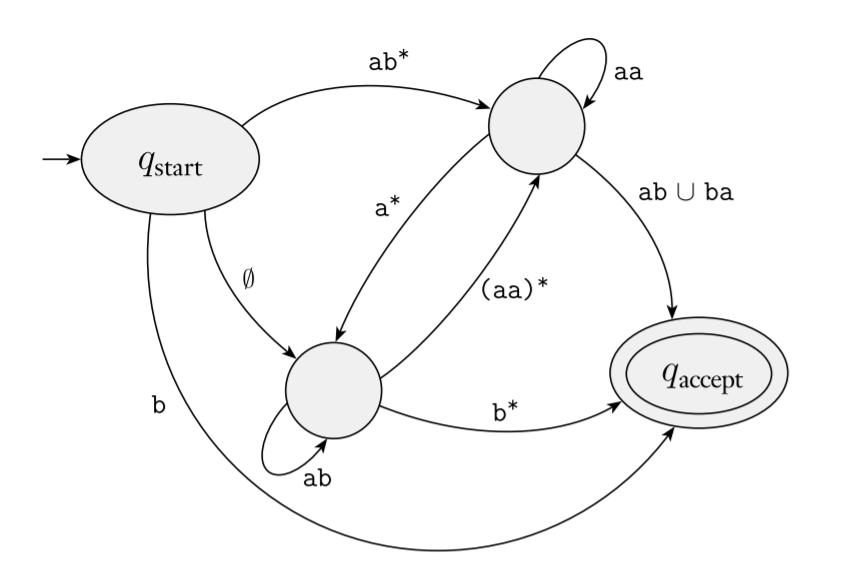
\includegraphics[scale=0.4]{assets/gnfa_ex_1.png}

    \textbf{Figure:} A generalized nondeterministic finite automaton.
\end{center}
We always require GNFAs to have a special form that meets the following conditions: 
\begin{enumerate}
    \item The \underline{start state} has transition arrows going to every other state but no arrows coming in from any other state. 
    \item There is only a single accept state, and it has arrows coming in from every other state but no arrows going to any other state. Additionally, the start state cannot be the accept state. 
    \item For all other states except the start/accept states, one arrow goes from every state to every other state and also from each state to itself. 
\end{enumerate}

\subsubsection{DFA to GNFA}
To convert a DFA to a GNFA, we do the following: 
\begin{itemize}
    \item We can add a new start state with a $\epsilon$ arrow to the old start state and a new accept state with $\epsilon$ from the old accept states. 
    \item If any arrows have multiple labels, or if there are multiple arrows going between the same two states in the same direction, replace each with a single arrow whose label is the union of the previous labels.
    \item Finally, add arrows labeled $\emptyset$ between states that have no arrows. 
\end{itemize}

\subsubsection{GNFA to Regular Expression}
We now need to convert a GNFA to a regular expression. Say that a GNFA has $k$ states. Then, because a GNFA must have a start and an accept state and they must be different from each other, we know that $k \geq 2$. If $k > 2$, we construct an equivalent GNFA with $k - 1$ states. We continue to do this until the GNFA is reduced to two states. If $k = 2$, then the GNFA has a single arrow that goes from the start state to the accept state. The label of this arrow would then be the \emph{equivalent regular expression}.

\bigskip 

The most important step in this process is constructing an equivalent GNFA with one fewer state when $k > 2$. How can we do this? Well: 
\begin{itemize}
    \item Select a state that isn't the start or accept state, rip that state out of the machine, and then repairing what is left of the machine so the same language is still recognized. Call this state $q_{\text{rip}}$.
    \item After removing $q_{\text{rip}}$, we need to repair the machine by altering the regular expressions that label each of the remaining arrows. We use these new labels because they add back the lost computations (from ripping $q_{\text{rip}}$). 
\end{itemize}
Consider the following GNFA: 
\begin{center}
    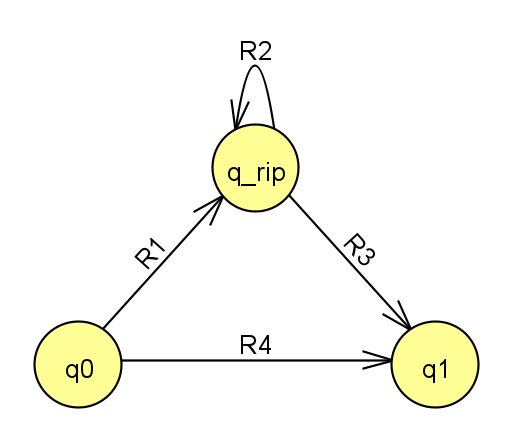
\includegraphics[scale=0.4]{assets/gnfa_before.png}
\end{center}
If we remove $q_{\text{rip}}$, we get the following GNFA: 
\begin{center}
    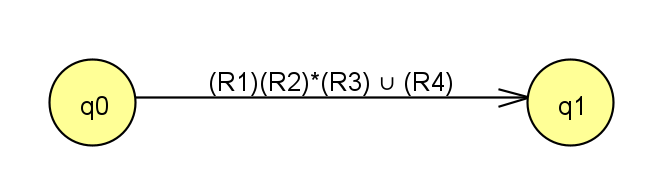
\includegraphics[scale=0.4]{assets/gnfa_after.png}
\end{center}
Essentially, in the old machine, if: 
\begin{enumerate}
    \item $q_0$ goes to $q_{\text{rip}}$ with an arrow labeled $R_1$, and 
    \item $q_{\text{rip}}$ goes to itself with an arrow labeled $R_2$, and 
    \item $q_{\text{rip}}$ goes to $q_1$ with an arrow labeld $R_3$, and 
    \item $q_0$ goes to $q_1$ with an arrow labeled $R_4$
\end{enumerate}
Then, in the new revised machine, the arrow from $q_0$ to $q_1$ gets the label 
\[(R_1)(R_2)^* (R_3) \cup (R_4)\]
We can make this change for each arrow going from any state $q_0$ to any state $q_1$, including when $q_0 = q_1$. 

\subsubsection{Formal Definition}
The formal definition of a GNFA is: 
\begin{definition}{Generalized Nondeterministic Finite Automaton}{}
    A \textbf{generalized nondeterministic finite automaton} is a 5-tuple $(Q, \Sigma, \delta, q_{\text{start}}, q_{\text{accept}})$ where 
    \begin{enumerate}
        \item $Q$ is the finite set of tuples. 
        \item $\Sigma$ is the input alphabet. 
        \item $\delta: (Q \setminus \{q_{\text{accept}}\}) \times (Q \setminus \{q_{\text{start}}\}) \mapsto \mathcal{R}$ is the transition function. 
        \item $q_{\text{start}}$ is the start state. 
        \item $q_{\text{accept}}$ is the accept state. 
    \end{enumerate}
\end{definition}
\textbf{Remarks:}
\begin{itemize}
    \item Here, $\mathcal{R}$ is the collection of all regular expressions over the alphabet $\Sigma$. 
    \item If $\delta(q_i, q_j) = R$, then the arrow from state $q_i$ to state $q_j$ has the regular expression $R$ as its label. 
\end{itemize}

\subsubsection{Convert Algorithm}
Suppose $G$ is an GNFA. Then, the $\code{CONVERT}(G)$ algorithm takes a GNFA and returns an equivalent regular expression. The algorithm works like so (Page 73): 
\begin{mdframed}[]
    $\code{CONVERT}(G)$
    \begin{enumerate}
        \item Let $k$ be the number of states of $G$. 
        \item If $k = 2$, then $G$ must consist of a start state, an accept state, and a single arrow connecting them and labeled with a regular expression $R$. So, return $R$. 
        \item Otherwise, $k > 2$ so we select any state $q_{\text{rip}} \in Q$ different from $q_{\text{start}}$ and $q_{\text{accept}}$. Let $G'$ be the GNFA $(Q', \Sigma, \delta', q_{\text{start}}, q_{\text{accept}})$ where $Q' = Q \setminus \{q_{\text{rip}}\}$ and, for any $q_i \in G' \setminus \{q_{\text{accept}}\}$ and $q_j \in Q' \setminus \{q_{\text{start}}\}$, let
        \[\delta'(q_i, q_j) = (R_1)(R_2)^* (R_3) \cup (R_4)\]
        Where $R_1 = \delta(q_i, q_{\text{rip}})$, $R_2 = \delta(q_{\text{rip}}, q_{\text{rip}})$, $R_3 = (q_{\text{rip}}, q_j)$, and $R_4 = \delta(q_i, q_j)$. 
        \item Compute $\code{CONVERT}(G')$. 
    \end{enumerate}
\end{mdframed}

\subsubsection{Example 1: DFA to Regular Expression}
Suppose we wanted to convert the following DFA to a regular expression:
\begin{center}
    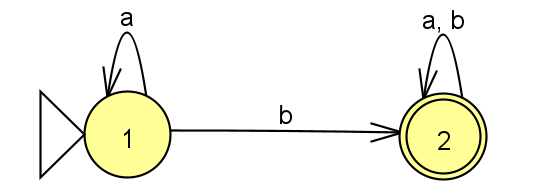
\includegraphics[scale=0.5]{assets/dfa_regex_1.png}
\end{center}

\begin{enumerate}
    \item First, we need to convert this DFA to a GNFA. This would look like: 
    \begin{center}
        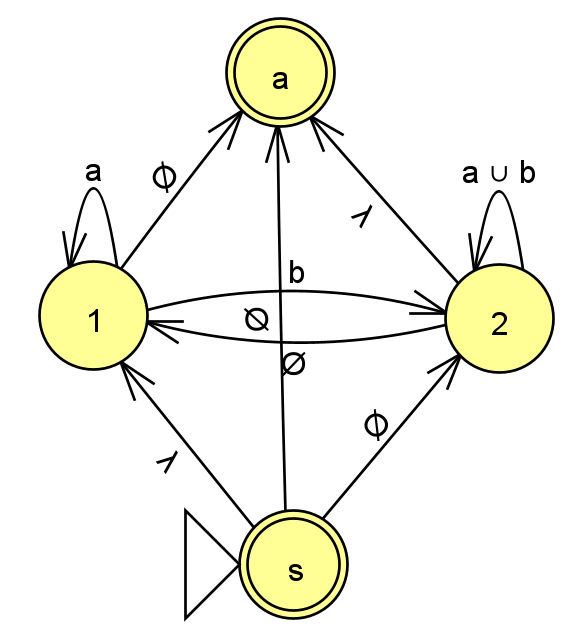
\includegraphics[scale=0.4]{assets/dfa_regex_2.png}
    \end{center}
    Here, we've made a few changes. 
    \begin{itemize}
        \item First, we added two new states: $s$ for the new \emph{start} state and $a$ for the new \emph{accept} state. We have an arrow from $s$ to $1$ (the old start state) with $\epsilon$ as its label\footnote{The software used to create these state machines use $\lambda$ instead of $\epsilon$.}. We also have an arrow from $2$ (the old accept state) to $a$ with $\epsilon$ as its label. 
        \item Next, note that there was an arrow labeled $a, b$ at state $2$. We take the \emph{union} of these two labels to get $a \cup b$. Thus, state $2$ now has an arrow with $a \cup b$ instead of $a, b$. This is because the DFA's label represents two transitions, but a GNFA may only have a single transition going from a state to itself. 
        \item Finally, we add several arrows with the labels being $\emptyset$:
        \begin{itemize}
            \item $2$ to $1$ since every state needs to be able to transition to all non-start states. 
            \item $1$ to $a$ for the same reason as above. 
            \item $s$ to $2$ for the same reason as above. 
            \item $s$ to $a$ for the same reason as above. 
        \end{itemize}
    \end{itemize}

    \item Next, we pick one non-start/accept state as $q_{\text{rip}}$. We'll pick $2$ for our case, so let $2 = q_{\text{rip}}$. We're going to make use of the \code{CONVERT} algorithm. So, we pick $q_i = 1$ and $q_j = a$. Then: 
    \begin{itemize}
        \item $\delta(q_i, q_{\text{rip}}) = R_1 = b$
        \item $\delta(q_{\text{rip}}, q_{\text{rip}}) = R_2 = a \cup b$
        \item $\delta(q_{\text{rip}}, q_j) = R_3 = \epsilon$
        \item $\delta(q_i, q_j) = R_4 = \emptyset$
    \end{itemize}
    Therefore, $\delta'(q_i, q_j) = (b)(a \cup b)^* \epsilon \cup \emptyset$. This simplifies to $\delta'(q_i, q_j) = (b)(a \cup b)^*$. So, the corresponding new state diagram is: 
    \begin{center}
        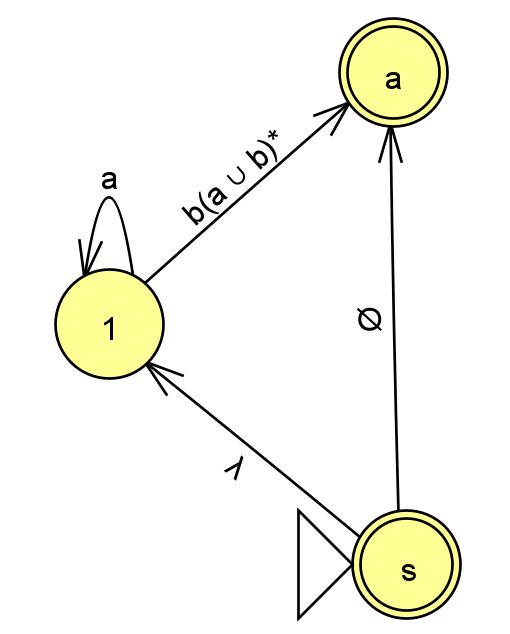
\includegraphics[scale=0.4]{assets/dfa_regex_3.png}
    \end{center}

    \item We do this process again. We pick our one non-start/accept state as $q_{\text{rip}} = 1$. By our algorithm again, let $q_i = s$ and $q_j = a$. Then: 
    \begin{itemize}
        \item $\delta(q_i, q_{\text{rip}}) = R_1 = \epsilon$
        \item $\delta(q_{\text{rip}}, q_{\text{rip}}) = R_2 = a$
        \item $\delta(q_{\text{rip}}, q_j) = R_3 = b(a \cup b)^*$
        \item $\delta(q_i, q_j) = R_4 = \emptyset$
    \end{itemize}
    Therefore, $\delta'(q_i, q_j) = (\epsilon)(a)^* b(a \cup b)^* \cup \emptyset$. This can be simplified to $\delta'(q_i, q_j) = (a)^* b(a \cup b)^*$. So, the corresponding new state diagram is:
    \begin{center}
        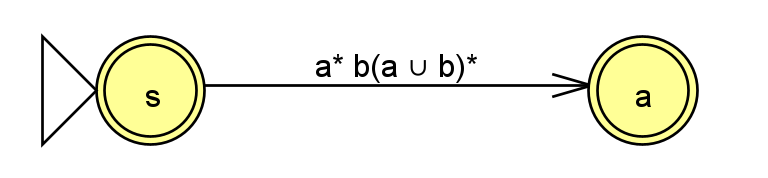
\includegraphics[scale=0.4]{assets/dfa_regex_4.png}
    \end{center}
    Thus, the regular expression corresponding to the given DFA is $\boxed{(a)^* b(a \cup b)^*}$
\end{enumerate}

% Ø  ∪ λ


\subsection{Regular Expressions and Regularity of Language}
\begin{theorem}{}{}
    A language is regular if and only if some regular expression describes it. 
\end{theorem}

\begin{mdframed}[]
    \begin{proof}
        The proof is given by the two lemmas. 
    \end{proof}    
\end{mdframed}

\subsubsection{Regular Expression Implies Regularity}

\begin{lemma}{}{}
    If a language is described by a regular expression, then it is regular. 
\end{lemma}

\begin{mdframed}[]
    \begin{proof}
        Suppose we convert $R$ into an NFA $N$. We then need to consider six cases as defined by the formal definition of regular expression.
        \begin{enumerate}
            \item Let $R = a$ for some $a \in \Sigma$. Then, $L(R) = \{a\}$ and the following NFA recognizes $L(R)$:
            \begin{center}
                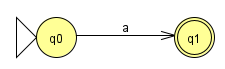
\includegraphics[scale=0.75]{assets/nfa_regex_pf_1.png}
            \end{center}
            
            \item Let $R = \epsilon$. Then, $L(R) = \{\epsilon\}$ and the following NFA recognizes $L(R)$:
            \begin{center}
                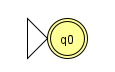
\includegraphics[scale=0.75]{assets/nfa_regex_pf_2.png}
            \end{center}

            \item Let $R = \emptyset$. Then, $L(R) = \emptyset$ and the following NFA recognizes $L(R)$:
            \begin{center}
                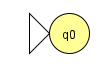
\includegraphics[scale=0.75]{assets/nfa_regex_pf_3.png}
            \end{center}

            \item $R = R_1 \cup R_2$
            \item $R = R_1 \circ R_2$
            \item $R = R_{1}^*$
        \end{enumerate}
        Where the last three cases is given by a previous proof. 
    \end{proof}
\end{mdframed}

\subsubsection{Regularity Implies Regular Expression}

\begin{lemma}{}{}
    If a language is regular, then it is described by some regular expression.
\end{lemma}

\begin{mdframed}[]
    \begin{proof}
        If the language is regular, then it is accepted by a DFA. From the above, we've given a sketch of how to convert a DFA to a regular expression. 
    \end{proof}
\end{mdframed}









































\newpage 
\section{Nonregular Languages (1.4)}
Of course, with great power comes great responsibility. This is certainly the case with finite automata. That is, we will prove that certain languages cannot be recognized by any finite automaton. Consider the language
\[B = \{\code{0}^n \code{1}^n \mid n \geq 0\}\]
It's not possible for us to find a finite automaton that recognizes $B$ simply because the machine needs to remember how many \code{0}s have been seen so far as it reads the input. In other words, because the number of \code{0}s is not limited, the machine would have to keep track of an \emph{unlimited} number of possibilities.

\begin{note}{}{}
    Just because the language appears to require unbounded memory doesn't mean that it is necessarily non-regular. For example, consider the two languages over $\Sigma = \{\code{0}, \code{1}\}$: 
    \[C = \{w \mid w \text{ has an equal number of \code{0}s and \code{1}s}\}\]
    \[D = \{w \mid w \text{ has an equal number of occurrences of \code{01} and \code{10} as substrings}\}\]
    $C$ is not regular, but $D$ \emph{is} regular, despise the fact that both languages require a machine that might need to keep count. 
\end{note}

\subsection{The Pumping Lemma}
We can use the concept known as the pumping lemma to prove nonregularity. In particular, this theorem states that all regular languages have a special property: the property that all strings in the language can be \emph{pumped} if they are at least as long as a certain special value, called the \textbf{pumping length}. This means that each string contains a section that can be repeated \emph{any number of times} with the resulting string remaining in the language. 

\bigskip 

So, if we can show that a language doesn't have this property, then it must be true that this language isn't regular. 

\begin{theorem}{Pumping Lemma}{}
    If $A$ is a regular language, then there is a number $p$ (the \emph{pumping length}) where if $s$ is any string in $A$ of length at least $p$, then $s$ may be divided into three pieces, $s = xyz$, satisfying the following conditions: 
    \begin{enumerate}
        \item For each $i \geq 0$, $xy^i z \in A$
        \item $|y| > 0$
        \item $|xy| \leq p$
    \end{enumerate}
\end{theorem}
\textbf{General Remarks:}
\begin{itemize}
    \item The pumping lemma is used to prove that a language is not regular. It cannot be used to prove that a language is regular. 
\end{itemize}
\textbf{Notational Remarks:}
\begin{itemize}
    \item Recall that $|s|$ represents the length of a string $s$.
    \item $y^i$ means that $i$ copies of $y$ are concatenated together. 
    \item $y^0 = \epsilon$.
    \item When $s$ is divided into $xyz$, either $x$ or $z$ may be $\epsilon$, but $y \neq \epsilon$ by condition 2. 
\end{itemize}

\subsection{Using Pumping Lemma in Proofs}
To prove that a language $L$ is not regular, we use the pumping lemma like so: 
\begin{enumerate}
    \item Assume that $L$ is regular so that the Pumping Lemma holds.
    \item Let $p$ be the pumping length for $L$ given by the lemma.
    \item Find a string $s \in L$ such that $|s| \geq p$. Your $s$ must be parametrized by $p$. \textbf{Warning:} Not every string in $L$ will work. 
    \item By the Pumping Lemma, there are strings $x$, $y$, $z$ such that all three conditions hold. Pick a particular $i \geq 0$ (usually, $i = 0$ or $i = 2$ will suffice) and show that $xy^i z \notin L$, thus yielding a contradiction. 
\end{enumerate}
Several points to consider:
\begin{itemize}
    \item Your proof must show that, for an \underline{arbitrary} $p$, there is a \underline{particular} string $s \in L$ (long enough) such that for \underline{any} split of $xyz$ (satisfying the conditions), there is an $i$ such that $xy^i z \notin L$. In other words, you must: 
    \begin{itemize}
        \item Assume a general $p$. You \textbf{cannot} choose a particular $p$.
        \item Find a concrete $s$. Your $s$ must be parametrized by $p$.
        \item Consider a general split $x, y, z$. You \textbf{cannot} choose a particular split; you must show every possible split.
        \item Show a particular $i$ for which the pumped word is not in $L$.  
    \end{itemize}
    \item The string $s$ does not need to be a random, representative member of $L$. It may come from a \emph{very specific} subset of $L$. For example, if your language is all strings with an equal number of \code{0}'s and \code{1}'s, your $s$ might be $0^p 1^p$.
    \item Make sure your string is long enough so that the first $p$ characters have a very limited form. 
    \item The vast majority of proofs use $i = 0$ or $i = 2$, but there are exceptions. 
\end{itemize}

\subsubsection{Example 1: Pumping Lemma Application}
We will show that the language $B$ described above is not regular.

\begin{mdframed}[]
    \begin{proof}
        Assume to the contrary that $B$ is regular. Then, let $p$ be the pumping length given by the pumping lemma. Let $s$ be the string $\code{0}^p \code{1}^p$. Because $s \in B$ and $|s| = 2p > p$, the pumping lemma guarantees that $s$ can be split into three pieces, $s = xyz$, where for any $i \geq 0$ the string $xy^i z \in B$. We now consider three cases to show that this is impossible. 
        \begin{enumerate}
            \item The string $y$ consists of only \code{0}s. In this case, the string $xyyz$ has more \code{0}s than \code{1}s and so is not a member of $B$, violating condition 1 of the pumping lemma. 
            \item The string $y$ consists of only \code{1}s. This also violates condition 1 of the pumping lemma. 
            \item The string $y$ consists of both \code{0}s and \code{1}s. In this case, the string $xyyz$ may have the same number of \code{0s} and \code{1}s, but they will be out of order since some \code{1}s will come before \code{0}s.
        \end{enumerate}
        Hence, a contradiction is unavoidable if we make the assumption that $B$ is regular. Thus, $B$ cannot be regular. 
    \end{proof}
\end{mdframed}
\textbf{Remark:} If we applied condition 3 of the Pumping Lemma, we could have removed case 2 and 3. An alternative proof is given below. 
\begin{mdframed}[]
    \begin{proof}
        Assume to the contrary that $B$ is regular. Then, let $p$ be the pumping length given by the pumping lemma. Let $s$ be the string $\code{0}^p \code{1}^p$. Because $s \in B$ and $|s| = 2p > p$, the pumping lemma guarantees that $s$ can be split into three pieces, $s = xyz$, where for any $i \geq 0$ the string $xy^i z \in B$. If our string looks like: 
        \[s = \overbrace{0000 \dots 0000}^{p \text{ times}} \overbrace{1111 \dots 1111}^{p \text{ times}}\]
        Then, we can split the string like so: 
        \[s = \underbrace{000}_{x}\overbrace{0 \dots 0000}^{y} \underbrace{1111 \dots 1111}_{z}\]
        Suppose $x$ has length $a$ and $y$ has length $b$ where $a + b \leq p$. Then, for $i = 2$, we have the string $xyyz$ where $xyy$ has length $a + b + b > p$ while $z$ has length $p$, a contradiction since we must have the same length of \code{0} and \code{1}. 
    \end{proof}
\end{mdframed}









































\newpage 
\section{Context-Free Grammars (2.1)}
Consider the following context-free grammar $G_1$:
\begin{equation*}
    \begin{aligned}
        A &\mapsto \code{0}A\code{1} \\ 
        A &\mapsto B \\ 
        B &\mapsto \code{\#}
    \end{aligned}
\end{equation*}
Here, we note the following:  
\begin{itemize}
    \item A grammar consists of a collection of \textbf{substitution rules} (also called productions). Each rule appears as a line in the grammar, comprising a symbol and a string separated by an arrow. 
    \item The symbol (e.g. $A$, $B$) is called a \textbf{variable}. They are often represented by capital letters.  
    \item The string consists of variables and other symbols (e.g. \code{0}, \code{1}, \code{\#}) called \textbf{terminals}. They are analogous to the input alphabet and often are represented by lowercase letters, numbers, or other special symbols. In other words, these are symbols that cannot be replaced (substituted). 
    \item One variable, usually (but not always) the top-left one in the list of rules (e.g. $A$), is designated as the \textbf{start variable}.
    \item When we have multiple rules with the same left-hand variable, we may condense them into a single line where the right-hand sides are separated by a \code{|} (as an ``or''). So, we can rewrite the above rules like so: 
    \begin{equation*}
        \begin{aligned}
            A &\mapsto \code{0}A\code{1} \mid B \\
            B &\mapsto \code{\#}
        \end{aligned}
    \end{equation*}
\end{itemize}
We can use a grammar to describe a language by generating each string of that language like so: 
\begin{enumerate}
    \item Write down the start variable. 
    \item Find a variable that is written down and a rule that starts with that variable. Then, replace the written dow nvariable with the right-hand side of that rule. 
    \item Repeat step 2 until no variables remain. 
\end{enumerate}

One \textbf{derivation} (the sequence of substitutions needed to obtain a string) is as follows:
\begin{equation*}
    \begin{aligned}
        A &\implies \code{0}A\code{1} && \text{By first rule.} \\ 
            &\implies \code{00}A\code{11} && \text{By first rule.} \\
            &\implies \code{000}A\code{111} && \text{By first rule.} \\
            &\implies \code{000}B\code{111} && \text{By second rule.} \\
            &\implies \code{000\#111} && \text{By third rule.} \\
    \end{aligned}
\end{equation*}

We say that all strings generated in this way constitute the \textbf{language of the grammar}, and write $L(G)$for the language of grammar $G$. So, for our introductory example above, we have that 
\[L(G_1) = \{\code{0}^n \code{\#} \code{1}^n \mid n \geq 0\}\]
We say that any language that can be generated by some context-free grammar is called a \textbf{context-free language} (CFL). 

\subsection{Formal Definition}
We now introduce the formal definition of a context-free grammar. 
\begin{definition}{Context-Free Grammar}{}
    A \textbf{context-free grammar} is a 4-tuple $(V, \Sigma, R, S)$ where 
    \begin{enumerate}
        \item $V$ is a finite set called the \textbf{variables}.
        \item $\Sigma$ is a finite set, disjoint from $V$, called the \textbf{terminals}.
        \item $R$ is a finite set of \textbf{rules}, with each rule being a variable and a string of variables and terminals.
        \item $S \in V$ is the start variable. 
    \end{enumerate}
\end{definition}
Suppose $u$, $v$, and $w$ are strings of variables and terminals.
\begin{center}
    \begin{tabular}{p{3in}|p{3in}}
        \textbf{Yielding} & \textbf{Deriving} \\ 
        \hline 
        Suppose $A \mapsto w$ is a rule of the grammar. Then, we say that $uAv$ \textbf{yields} $uwv$, written $uAv \implies uwv$. &
        We say that $u$ \textbf{derives} $v$, written $u \stackrel{*}{\implies}$, if $u = v$ or if a sequence $u_1, u_2, \dots, u_k$ exists for $k \geq 0$ and 
        \[u \implies u_1 \implies u_2 \implies \dots \implies u_k \implies v\]
    \end{tabular}
\end{center}
So, it follows that the \textbf{language of the grammar} is given by 
\[\{w \in \Sigma^* \mid S \stackrel{*}{\implies} w\}\]

\subsection{Closure Properties of CFGs}
There are several closure properties which may be helpful. Suppose we have two CFGs $G_1$ and $G_2$, with start states $S_1$ and $S_2$, respectively. 
\begin{itemize}
    \item \underline{Union:} Suppose we wanted to generate a CFG for the language $L(G_1) \cup L(G_2)$. This is as simple as making a new start variable: 
    \[S \mapsto S_1 \mid S_2\]

    \item \underline{Concatenation:} Suppose we wanted to generate a CFG for the language $L(G_1) \circ L(G_2)$. This is as simple as making a new start variable:
    \[S \mapsto S_1 S_2\]

    \item \underline{Kleene Star:} Suppose we wanted to generate a CFG for the language $L(G_1)^*$. This is as simple as making a new start variable:
    \[S \mapsto S S_1 \mid \epsilon\]
\end{itemize}

\subsubsection{Example 1: Identifying Language}
Consider the grammar $G_3 = (\{S\}, \{\code{a}, \code{b}\}, R, S)$, with $R$ being the rule 
\[S \mapsto \code{a}S\code{b} | SS | \epsilon\]
Describe the language of this context-free grammar. 

\begin{mdframed}[]
    This grammar generates strings like \code{abab}, \code{aaabbb}, and \code{aababb}. We can describe the language $L(G_3)$ as all strings where, for any \code{a}, there is a corresponding \code{b}. Analogously, if we let \code{a} be \code{(} and \code{b} be \code{)}, then this is the language of all properly nested parentheses. 
\end{mdframed}

\subsection{Describing Context-Free Languages}
Many context-free languages are the union of simpler context-free languages. So, if you need to construct a context-free grammar for a context-free language, break it into simpler pieces, create the corresponding grammars, and then merge them into a grammar for the original language by combining their rules and then adding the new rule 
    \[S \mapsto S_1 \mid S_2 \mid \dots \mid S_k\]
where the variables $S_i$ are the start variables for the individual grammars. 

\subsubsection{Example 1: Constructing Context-Free Grammar}
Build a CFG to describe the language $\{\code{abba}\}$. 

\begin{mdframed}[]
    There are several ways to go about this. Consider
    \[G_a = (\{S\}, \{\code{a}, \code{b}\}, \{S \mapsto \code{abba}\}, S)\]
    which maps $S$ to \code{abba}, exactly what we wanted. 

    \bigskip 

    Another example is 
    \[G_b = (\{S, T, V, W\}, \{\code{a}, \code{b}\}, R, S)\]
    where $R$ is defined by the rules 
    \begin{equation*}
        \begin{aligned}
            S &\mapsto \code{a}T \\ 
            T &\mapsto \code{b}V \\ 
            V &\mapsto \code{b}W \\ 
            W &\mapsto \code{a}
        \end{aligned}
    \end{equation*}
    So, if we applied the substitution rules, we would get 
    \begin{equation*}
        \begin{aligned}
            S &\mapsto \code{aT} && \text{By first rule.} \\ 
                &\mapsto \code{ab}V && \text{By second rule.} \\ 
                &\mapsto \code{abb}W && \text{By third rule.} \\ 
                &\mapsto \code{abba} && \text{By fourth rule.}
        \end{aligned}
    \end{equation*}
\end{mdframed}

\subsubsection{Example 2: Constructing Context-Free Grammar}
Build a CFG to describe the language $\{\code{0}^n \code{1}^n \mid n \geq 0\} \cup \{\code{1}^n \code{0}^n \mid n \geq 0\}$. 

\begin{mdframed}[]
    First, construct the grammar for $\{\code{0}^n \code{1}^n \mid n \geq 0\}$. We note that some strings in this grammar are $\epsilon$, \code{01}, \code{0011}, and so on. So, the CFG would be  
    \[S_1 \mapsto \code{0}S_1 \code{1} \mid \epsilon\]
    Likewise, construct the grammar for $\{\code{1}^n \code{0}^n \mid n \geq 0\}$, which gives us 
    \[S_2 \mapsto \code{1}S_2 \code{0} \mid \epsilon\]
    So, our solution is 
    \begin{equation*}
        \begin{aligned}
            S &\mapsto S_1 \mid S_2 \\ 
            S_1 &\mapsto \code{0}S_1 \code{1} \mid \epsilon \\ 
            S_2 &\mapsto \code{1}S_2 \code{0} \mid \epsilon
        \end{aligned}
    \end{equation*}
\end{mdframed}


\subsection{Relation Between CFGs and Regular Languages}
We know that every regular language is also a context-free language (\emph{however}, not every context-free language is a regular language). There are two approaches to show that this is the case.
\begin{enumerate}
    \item Start with an arbitrary DFA $M$, then build a CFG that generates $L(M)$. 
    \item Build CFGs for $\{\code{a}\}$, $\{\epsilon\}$, and $\emptyset$. Then, show that the class of context-free languages is closed under the regular operations (union, concatenation, Kleene star). 
\end{enumerate}

\subsubsection{First Approach}
\begin{proposition}
    Given any DFA $M$, there is a CFG whose language is $L(M)$. 
\end{proposition}

\begin{mdframed}[nobreak=true]
    \begin{proof}
        Given a DFA $M = (Q, \Sigma, \delta, q_0, F)$, we can define the CFG $G = (V, \Sigma, R, S)$ where 
        \begin{itemize}
            \item $V = \{S_i \mid q_i \in Q\}$
            \item $R = \{S_i \mapsto \code{a}S_j \mid \delta(q_i, \code{a}) = q_j\} \cup \{S_i \mapsto \epsilon \mid q_i \in F\}$
            \item $S = S_0$
        \end{itemize}
        From this, we need to prove correctness.
    \end{proof}
\end{mdframed}

\subsubsection{Second Approach}
We can build CFGs for $\{\code{a}\}$, $\{\epsilon\}$, and $\emptyset$. Then, show that the class of context-free languages is closed under the regular operations (union, concatenation, Kleene star). 

\begin{itemize}
    \item If $L = \{\code{a}\}$, where \code{a} is some arbitrary character in the alphabet, then we have the CFG $(V, \Sigma, R, S)$ where 
    \begin{itemize}
        \item $V = \{S\}$
        \item $R = \{S \mapsto \code{a}\}$
    \end{itemize}
    
    \item If $L = \{\epsilon\}$, then we have the CFG $(V, \Sigma, R, S)$ where 
    \begin{itemize}
        \item $V = \{S\}$
        \item $R = \{S \mapsto \epsilon\}$
    \end{itemize}
    
    \item If $L = \emptyset$, then we have the CFG $(V, \Sigma, R, S)$ where 
    \begin{itemize}
        \item $V = \{S\}$
        \item $R =  \emptyset$ (or $R = \{S \mapsto S\}$)
    \end{itemize} 
\end{itemize}
Suppose we have $G_1 = \{V_1, \Sigma, R_1, S_1\}$ and $G_2 = \{V_2, \Sigma, R_2, S_2\}$, where $G_1$ describes the language $L_1$ and $G_2$ describes the language $L_2$, then we can describe $L_1 \cup L_2$ by combining the grammars to make the grammar $G = (V, \Sigma, R, S)$ where:
\begin{itemize}
    \item $V = V_1 \cup V_2 \cup \{S\}$ (where we assume that $V_1 \cap V_2 = \emptyset$)
    \item $R = R_1 \cup R_2 \cup \{S \mapsto S_1 \mid S_2\}$
\end{itemize}

\subsection{More Examples of CFG Construction}
We now discuss some examples of CFG construction.

\subsubsection{Example 1: Basic Construction}
Build a CFG to describe the language $\{\code{0}^n \code{1}^n \mid n \geq 0\} \cup \{\code{1}^n \code{0}^n \mid n \geq 0\}$. 

\begin{mdframed}[]
    First, construct the grammar for $\{\code{0}^n \code{1}^n \mid n \geq 0\}$. We note that some strings in this grammar are $\epsilon$, \code{01}, \code{0011}, and so on. So, the CFG would be  
    \[S_1 \mapsto \code{0}S_1 \code{1} \mid \epsilon\]
    Likewise, construct the grammar for $\{\code{1}^n \code{0}^n \mid n \geq 0\}$, which gives us 
    \[S_2 \mapsto \code{1}S_2 \code{0} \mid \epsilon\]
    So, our solution is 
    \begin{equation*}
        \begin{aligned}
            S &\mapsto S_1 \mid S_2 \\ 
            S_1 &\mapsto \code{0}S_1 \code{1} \mid \epsilon \\ 
            S_2 &\mapsto \code{1}S_2 \code{0} \mid \epsilon
        \end{aligned}
    \end{equation*}
\end{mdframed}

\subsubsection{Example 2: Advanced Construction}
Build a CFG to describe the langauge $\{0^n 1^m 2^n \mid n, m \geq 0\}$.

\begin{mdframed}[]
    We begin by considering some strings that are generated by this CFG. In particular, we have \code{02}, \code{1}, \code{012}, \code{0112}, \code{00122}, and so on. We know that there are an equal number of \code{0}'s and \code{2}'s, so our start rule must have at least 
    \[S \mapsto \code{0}S\code{2}\]
    What if we have no more $n$ though? We now need to consider the \code{1}s. So, we can create another rule 
    \[T \mapsto \code{1}T\] 
    But, since we can have 0 \code{1}'s, we also need to include the empty string; therefore, our rule for $T$ is 
    \[T \mapsto \code{1}T \mid \epsilon\]
    And, thus, our final set of rules are 
    \[S \mapsto \code{0}S\code{2}\]
    \[T \mapsto \code{1}T \mid \epsilon\]
    To show that this works, note that we will always have the same number of \code{0}'s and \code{2}'s. After we expend all of those, then we can consider some number of \code{1}'s (which we may not necessarily have the same amount of as \code{0}'s and \code{2}'s). Finally, we note that $S$ can map straight to $\epsilon$, implying that the empty string is something that is generated from this language (and, indeed, this is true if $n = m = 0$).
\end{mdframed}

\subsubsection{Example 3: Wild Generations}
Consider the CFG $G = (V, \Sigma, R, S)$ defined by
\begin{itemize}
    \item $V = \{E\}$
    \item $\Sigma = \{\code{1}, +, \times, (, )\}$
    \item $R = \{E \mapsto E + E \mid E \times E \mid (E) \mid \code{1}\}$
    \item $S = E$
\end{itemize}

Which of the following strings is/are generated by this CFG?
\begin{enumerate}[\hspace{0.5cm}a.]
    \item E
    \item \code{11}
    \item $\code{1} + \code{1} \times \code{1}$
    \item $\epsilon$
\end{enumerate}

\begin{mdframed}[]
    The answer is \textbf{C}. The reason why is because we can perform the following substitutions:
    \begin{equation*}
        \begin{aligned}
            E &\implies E + E && \text{By the first rule.} \\ 
                &\implies \code{1} + E && \text{By the last rule.} \\ 
                &\implies \code{1} + E \times E && \text{By the second rule.} \\ 
                &\implies \code{1} + \code{1} \times E && \text{By the last rule.} \\ 
                &\implies \code{1} + \code{1} \times \code{1} && \text{By the last rule.}
        \end{aligned}
    \end{equation*}
    Note that there are potentially other possible ways this string can be generated. Regardless, the answer is not A because a variable is not a valid string. The answer is not B because there is no way to expand $E$ out twice. The answer is not D because you cannot generate the empty string with the given rules. 
\end{mdframed}

\subsection{Ambiguity}
Sometimes, a grammar can generate the same string in several different ways.
\begin{definition}{Grammar Ambiguity}{}
    A string $w$ is derived \textbf{ambiguously} in a context-free grammar $G$ if it has two or more leftmost derivations\footnote{We say that a derivation of a string $w$ in a grammar $G$ is a \textbf{leftmost derivation} if, at every step, the leftmost remaining variable is the one replaced.}. Grammar $G$ is ambiguous if it generates some string ambiguously.
\end{definition}
For example, consider the last example discussed above. There are several ways to derive $\code{1} + \code{1} \times \code{1}$. Some examples are shown below. 
\begin{mdframed}[]
    \begin{itemize}
        \item Derivation 1:
        \begin{equation*}
            \begin{aligned}
                E &\implies E + E && \text{By the first rule.} \\ 
                    &\implies \code{1} + E && \text{By the last rule.} \\ 
                    &\implies \code{1} + E \times E && \text{By the second rule.} \\ 
                    &\implies \code{1} + \code{1} \times E && \text{By the last rule.} \\ 
                    &\implies \code{1} + \code{1} \times \code{1} && \text{By the last rule.}
            \end{aligned}
        \end{equation*}

        \item Derivation 2: 
        \begin{equation*}
            \begin{aligned}
                E &\implies E + E && \text{By the first rule.} \\ 
                    &\implies E + E \times E && \text{By the second rule.} \\ 
                    &\implies 1 + E \times E && \text{By the last rule.} \\ 
                    &\implies 1 + 1 \times E && \text{By the last rule.} \\ 
                    &\implies 1 + 1 \times 1 && \text{By the last rule.}
            \end{aligned}
        \end{equation*}
    \end{itemize}
\end{mdframed}
Note that some context-free languages can be generated only by ambiguous grammars; in this case, we say that these languages are \textbf{inherently ambiguous}.

\subsection{Chomsky Normal Form}
We can use Chomsky normal form to ``simplify'' a context-free grammar. 
\begin{definition}{Chomsky Normal Form}{}
    A context-free grammar is in \textbf{Chomsky normal form} if every rule is of the form 
    \begin{equation*}
        \begin{aligned}
            A &\mapsto BC \\ 
            A &\mapsto a
        \end{aligned}
    \end{equation*}
    where a is any terminal and $A, B, C$ are any variables, except that $B$ and $C$ may not be the start variables. In addition, we permit the rule $S \mapsto \epsilon$, where $S$ is the start variable.  
\end{definition}

A somewhat important theorem is as follows:
\begin{theorem}{}{}
    Any context-free language is generated by a context-free grammar in Chomsky normal form. 
\end{theorem}









































\newpage 
\section{Pushdown Automata (2.2)}
We now introduce a new type of computational model called the \textbf{pushdown automata}, which is essentially like a nondeterministic finite automata but with an extra component called a \textbf{stack}. The stack provides additional memory beyond the finite amount available in the control, additionally allowing us to recognize some nonregular languages. 

\bigskip 

Note that pushdown automata are \underline{equivalent in power} to context-free grammars, giving us the ability to decide which of the two we want to use to prove that a language is context-free. 


\subsection{The Idea}
The idea is that, at each step: 
\begin{enumerate}
    \item \textbf{Transition} to a new state based on the current state, letter read, \emph{and} the top letter of the stack. 
    \item Possibly push (or pop) a letter to (or from) the top of the stack. 
\end{enumerate}
We \emph{accept} a string if there is \textbf{some} sequence of states and \textbf{some} sequence of stack contents which processes the entire input string and ends in an accepting state. We assume that the stack is empty at the beginning, and don't necessarily care if the stack is empty at the end.

\subsection{Formal Definition}
As implied, the formal definition of a pushdown automaton is similar to that of a finite automaton, except for the stack. The stack is a device containing symbols drawn from some alphabet, and the machine may use different alphabets for its input and its stack. Therefore, we need to specify both an input alphabet $\Sigma$ and a stack alphabet $\Gamma$. 

\bigskip 

Recall that $\Sigma_{\epsilon} = \Sigma \cup \{\epsilon\}$; the same idea applies with $\Gamma_{\epsilon}$. Now, the domain of $\delta$ is $Q \times \Sigma_{\epsilon} \times \Gamma_{\epsilon}$. The idea behind this domain is that, given the current state $q \in Q$, next input symbol read $\sigma \in \Sigma_{\epsilon}$, and top symbol of the stack $\gamma \in \Gamma_{\epsilon}$, the machine can decide the next move. As usual, if $\sigma = \epsilon$, then the machine won't read a symbol from the input. Likewise, if $\gamma = \epsilon$, then the machine won't read a symbol from the stack.  

\bigskip 

We now consider the range of the $\delta$ function. It's possible that it can enter a new state and possibly write a symbol on top of the stack. This is indicated by some member of $Q \times \Gamma_{\epsilon}$. 

\begin{definition}{Pushdown Automaton (PDA)}{}
    A \textbf{pushdown automaton} is a 6-tuple $(Q, \Sigma, \Gamma, \delta, q_0, F)$, where $Q$, $\Sigma$, $\Gamma$, and $F$ are all finite sets, and
    \begin{enumerate}
        \item $Q$ is the set of states. 
        \item $\Sigma$ is the input alphabet. 
        \item $\Gamma$ is the stack alphabet.
        \item $\delta: Q \times \Sigma_{\epsilon} \times \Gamma_{\epsilon} \mapsto \PowerSet(Q \times \Gamma_{\epsilon})$ is the transition function.
        \item $q_0 \in Q$ is the start state. 
        \item $F \subseteq Q$ is the set of accept states. 
    \end{enumerate} 
\end{definition}
\textbf{Remark:} We write $a, b \mapsto c$ to signify that, when the machine is reading an $a$ from the input, it may replace the symbol $b$ on the top of the stack with a $c$; in other words, pop $b$ and push $c$. 
\begin{itemize}
    \item If $a = \epsilon$, then the machine may make this transition without reading any symbol from the input. 
    \item If $b = \epsilon$, then the machine may make this transition without readng any symbols from the stack, but it will push $c$ onto the stack. 
    \item If $c = \epsilon$, then the machine will pop $b$ from the stack but not push anything to the stack. 
\end{itemize}
\textbf{Note:} The formal definition of a PDA contains no explicit mechanism to allow the PDA to test for an empty stack. So, one trick that we can do is to initially push a special symbol \code{\$} on the stack. Then, if it ever sees the \code{\$} again, then it knows that the stack is effectively empty. 

\subsection{Computation of a Pushdown Automaton}
A pushdown automaton $M = (Q, \Sigma, \Gamma, \delta, q_0, F)$ accepts input $w$ if $w$ can be written as $w = w_1 w_2 \dots w_m$, where each $w_i \in \Sigma_{\epsilon}$ and the sequences of starts $r_0, r_1, \dots, r_m \in Q$ and strings $s_0, s_1, \dots, s_m \in \Gamma^*$ exist that satisfy the following three conditions.
\begin{enumerate}
    \item $r_0 = q_0$ and $s_0 = \epsilon$, which signifies that $M$ starts out properly, in the start state, and with an empty stack. 
    \item For $i = 0, \dots, m - 1$< we have $(r_{i + 1}, b) \in \delta(r_i, w_{i + 1}, a)$, where $a_i = at$ and $s_{i + 1} = bt$ for some $a, b \in \Gamma_{\epsilon}$ and $t \in \Gamma^*$. This condition states that $M$ moves properly according to the state, stack, and next input symbol. 
    \item $r_m \in F$. This condition states that the accept state occurs at the input end. 
\end{enumerate}

\subsection{Context-Free}
\begin{theorem}{}{}
    A language is context free if and only if some pushdown automaton recognizes it.
\end{theorem}

\subsubsection{Example 1: Designing a PDA}
Consider the following language $L = \{\code{0}^i \code{1}^{i + 1} \mid i \geq 0\}$. 

\begin{enumerate}
    \item Design a CFG that generates $L$. 
    \begin{mdframed}[]
        We can define a CFG $G$ where the rules are 
        \begin{equation*}
            \begin{aligned}
                S &\mapsto T\code{1} | \code{0}S\code{1} \\ 
                T &\mapsto \epsilon
            \end{aligned}
        \end{equation*}
        The idea is that $S$ can recursively map to $\code{0}S\code{1}$. After enough times, it can then map to $T\code{1}$, which adds one more \code{1}. 
    \end{mdframed}

    \item Consider the notation $\epsilon, \epsilon \mapsto \code{\$}$. What does this mean? 
    \begin{mdframed}[]
        Without reading any input, and without popping any symbols from the stack, we push \code{\$} on top of the stack. 
    \end{mdframed}
    \textbf{Remark:} This is commonly used from the initial state (at the start of computation) to record the top of the stack with a special symbol. In other words, if the stack becomes empty, then we will know. 

    \item Provide a rough description of how you can make a PDA that accepts upon receiving any strings that are in this language. 
    \begin{mdframed}[]
        The idea for a PDA is that we need to read the symbols from the input. As each \code{0} is read, we push it onto the stack. As soon as \code{1}'s are seen, we pop a \code{0} for each \code{1} that is read. If the stack becomes empty and there is exactly one \code{1} left to read, then we read that \code{1} and accept the input. If the stack becomes empty and there are either zero or more than one \code{1}'s left to read, \emph{or} if the \code{1}'s are finished while the stack still contains \code{0}'s, \emph{or} if any \code{0}'s appear in the input following the \code{1}'s, then reject the input. 
    \end{mdframed}

    \item Design a PDA that does exactly what you described in the previous step. 
    \begin{mdframed}[nobreak=true]
        \begin{center}
            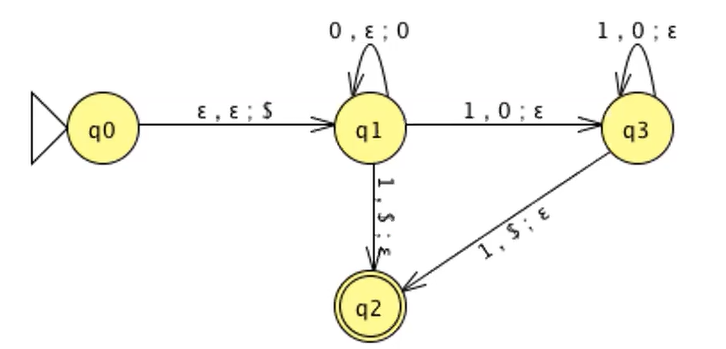
\includegraphics[scale=0.7]{assets/pda_1.png}
        \end{center}
    \end{mdframed}

    \item Describe how your PDA works with the input \code{00111}.
    \begin{mdframed}[]
        \begin{itemize}
            \item For our initial step, we start at $q_0$ and our stack can be described as \code{[]}.
            \item Looking at the only transition arrow, note that we can transition without reading any input ($\epsilon, \epsilon \mapsto \$$). Upon transitioning, we don't pop anything from the stack, but we do push the special \code{\$} onto the stack. So, we can describe the machine like so: 
            \begin{verbatim}
                State:  q1
                Stack:  [$]     Top 
                Input:  00111
                        ^
            \end{verbatim}

            \item At $q_1$, we have three transition arrows; one that requires a \code{0} (without reading and popping anything from the stack), and two that requires a \code{1} (one which requires the \code{\$} to be at the top of the stack, and another that requires a \code{0} to be on top of the stack). As the (first and) next symbol in our input is \code{0}, we read that in and transition to $q_1$ again while also pushing \code{0} onto the stack. 
            \begin{verbatim}
                State:  q1
                Stack:  [$, 0]     Top 
                Input:  00111
                         ^         Next to read
            \end{verbatim}

            \item We repeat the previous step since we need to read in a \code{0}. 
            \begin{verbatim}
                State:  q1
                Stack:  [$, 0, 0]     Top 
                Input:  00111
                          ^           Next to read
            \end{verbatim}

            \item At this point, our next input symbol is \code{1}. As we're at $q_1$ still, we now need to consider the two transition arrows that can read in a \code{1}. One transition arrow requires a \code{0} to be on top of the stack, and another requires a \code{\$}. So, we go with the one that requires a \code{0} to be on top of the stack since that's what we have in the stack. So, we transition to $q_3$, popping a \code{0} from the stack. 
            \begin{verbatim}
                State:  q2
                Stack:  [$, 0]     Top 
                Input:  00111
                           ^       Next to read
            \end{verbatim}
            
            \item We are now at state $q_3$. The next input symbol we need to read in is the \code{1} (the center one), and we still have another \code{0} on top of the stack. So, we take the transition arrow $\code{1}, \code{0} \mapsto \epsilon$. After transitioning back to $q_3$, we pop \code{0} from the stack. 
            \begin{verbatim}
                State:  q2
                Stack:  [$]     Top 
                Input:  00111
                            ^   Next to read
            \end{verbatim}

            \item Now that we're still at $q_3$, we still need to read in \code{1} (the last one). However, the top of the stack is a \code{\$}, implying that we're at the end of the stack. We note that there is a transition arrow $\code{1}, \$ \mapsto \epsilon$, we take that transition arrow. So, we transition to $q_2$ and pop \code{\$} from the stack. 
            \begin{verbatim}
                State:  q2
                Stack:  []     Top 
                Input:  00111
                             ^ Next to read
            \end{verbatim}

            \item There is nothing left to read, and since we're at $q_2$, we accept.
        \end{itemize}

        For a summary of what just happened, observe the below table.
        \begin{center}
            \begin{tabular}{c|c|c}
                \textbf{Input} & $q$ & \textbf{Stack} (Top is Right) \\ 
                \hline 
                               & $q_0$ & \code{[]} \\ 
                               & $q_1$ & \code{[\$]} \\ 
                \code{0}       & $q_1$ & \code{[\$, 0]} \\ 
                \code{0}       & $q_1$ & \code{[\$, 0, 0]} \\ 
                \code{1}       & $q_3$ & \code{[\$, 0]} \\ 
                \code{1}       & $q_3$ & \code{[\$]} \\ 
                \code{1}       & $q_2$ & \code{[]} \\ 
            \end{tabular}
        \end{center}
    \end{mdframed}
\end{enumerate}

\subsubsection{Example 2: PDA vs. CFGs}
Consider the following language $L = \{\code{a}^i \code{b}^j \code{c}^k \mid i = j \text{ or } i = k \text{ with } i, j, k \geq 0\}$. 

\begin{enumerate}
    \item Which of the following strings are \textbf{not} in $L$?
    \begin{itemize}
        \item \code{b}
        \item \code{abc}
        \item \code{abbcc}
        \item \code{aabcc}
    \end{itemize}

    \begin{mdframed}[]
        The answer is \code{abbcc}. This says that $i = 1$, $j = k = 2$, but this violates the definition that $i = j$ or $i = k$ since $i \neq j$ and $i \neq k$. 
    \end{mdframed}


    \item Create a CFG that generates $L$. 
    \begin{mdframed}[]
        The idea is that 
        \begin{equation*}
            \begin{aligned}
                L &= \{\code{a}^i \code{b}^j \code{c}^k \mid i = j \text{ or } i = k \text{ with } i, j, k \geq 0\} \\ 
                    &= \{\code{a}^i \code{b}^j \code{c}^k \mid i = j \text{ with } i, j, k \geq 0\} \cup \{\code{a}^i \code{b}^j \code{c}^k \mid i = k \text{ with } i, j, k \geq 0\}
            \end{aligned}
        \end{equation*}
        So, we can find the CFG of each individual language and then combine them to form the CFG of interest. 

        \begin{itemize}
            \item $L_1 = \{\code{a}^i \code{b}^j \code{c}^k \mid i = j \text{ with } i, j, k \geq 0\}$. The CFG can be defined by 
            \begin{equation*}
                \begin{aligned}
                    A &\mapsto A\code{c} \mid B \\ 
                    B &\mapsto \code{a}B\code{b} \mid \epsilon
                \end{aligned}
            \end{equation*}

            \item $L_2 = \{\code{a}^i \code{b}^j \code{c}^k \mid i = k \text{ with } i, j, k \geq 0\}$. The CFG can be defined by 
            \begin{equation*}
                \begin{aligned}
                    C &\mapsto \code{a}C\code{c} \mid D \\ 
                    D &\mapsto D\code{b} \mid \epsilon
                \end{aligned}
            \end{equation*}
        \end{itemize}

        Combining these gives us 
        \begin{equation*}
            \begin{aligned}
                S &\mapsto A \mid C \\ 
                A &\mapsto A\code{c} \mid B \\ 
                B &\mapsto \code{a}B\code{b} \mid \epsilon \\ 
                C &\mapsto \code{a}C\code{c} \mid D \\ 
                D &\mapsto D\code{b} \mid \epsilon
            \end{aligned}
        \end{equation*}
    \end{mdframed}

    \item Give an informal description of a PDA that accepts all strings in this language. \emph{Hint:} Consider what information you need to track, the amount of memory you need, and whether non-determinism is needed.
    
    \begin{mdframed}[]
        \begin{itemize}
            \item The PDA pushes a \code{\$} to indicate the top of the stack. Then, it starts reading \code{a}'s, pushing each one onto the top of the stack.
            \item The PDA then guesses when it has reached the end of the \code{a}'s and whether to match the number of \code{a}'s to the number of \code{b}'s or the number of \code{c}'s. 
            \item If trying to match number of \code{b}'s with the number of \code{a}'s, the PDA pops off \code{a}'s for each \code{b} that is read in. If there are more \code{a}'s on the stack but no more \code{b}'s being read, then we reject. When the end of the stack \code{\$} is reached, the number of \code{a}'s matches the number of \code{b}'s. If this is the end of the input or if any number of \code{c}'s is read at this point, accept. Otherwise, reject. 
            \item If trying to match the number of \code{c}'s with the number of \code{a}'s, first read any number of \code{b}'s without changing the stack content. Then, nondeterministically guess when to start reading the \code{c}'s. For each \code{c} read, pop one \code{a} off the stack. When the end of the stack \code{\$} is reached, the number of \code{a}'s and \code{c}'s match. 
        \end{itemize}
    \end{mdframed}

    \item Design a PDA that does exactly what you described in the previous step. 
    \begin{mdframed}[nobreak=true]
        \begin{center}
            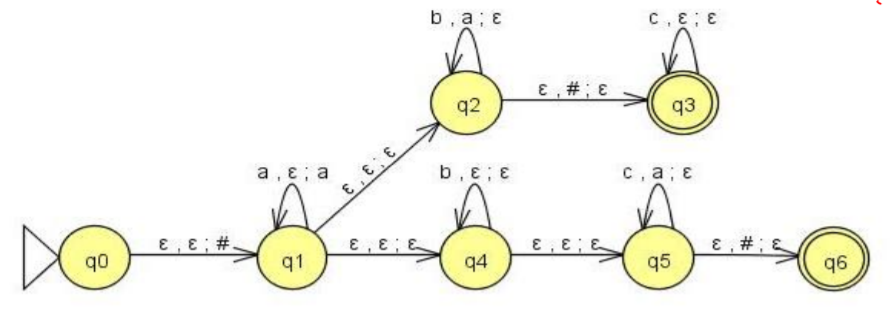
\includegraphics[scale=0.6]{assets/pda_2.png}
        \end{center}
    \end{mdframed}
\end{enumerate}


\subsubsection{Example 3: PDA vs. CFGs}
Consider the language 
\[L = \{x\code{\#}w \mid x, w \in \{\code{0}, \code{1}\}^* \text{ and } w^R \text{ is a substring of } x\}\]

\begin{enumerate}
    \item Recall that a CFG is a 4-tuple $(V, \Sigma, R, S)$. Here, $\Sigma = \{\code{0}, \code{1}, \code{\#}\}$ and $S \in V$. What is $V$ and $R$?
    \begin{mdframed}[]
        Let's consider some example strings. 
        \begin{itemize}
            \item \code{\#}
            \item \code{0\#0}
            \item \code{1011\#110}
            \item \code{0100101\#1010}
        \end{itemize}
        In particular, we note several things. 
        \begin{itemize}
            \item $|x| \geq |w|$. This means we can add some number of \code{0}'s or \code{1}'s to the left side of the \code{\#} without adding them to the right side. 
            \item At some point, when we generate the string, we're just adding \code{0} (or \code{1}) to the ends of both sides. 
        \end{itemize}
        So, we can define $R$ like so: 
        \begin{equation*}
            \begin{aligned}
                S &\mapsto \code{0}S \mid \code{1}S \mid A \\ 
                A &\mapsto \code{0}A\code{0} \mid \code{1}A\code{1} \mid B\code{\#} \\ 
                B &\mapsto \code{0}B \mid \code{1}B \mid \epsilon
            \end{aligned}
        \end{equation*}
        Therefore, $V$ is given by 
        \[V = \{S, A, B\}\]
    \end{mdframed}

    \item Give an informal description of a PDA that accepts all strings in this language. 
    \begin{mdframed}[]
        We're going to take a non-deterministic approach to this problem. Essentially, the idea is as follows: 
        \begin{itemize}
            \item The PDA pushes a \code{\$} to indicate the top of the stack. 
            \item Then, it starts reading \code{0}'s and \code{1}'s without adding or removing anything from the stack. This accounts for the possibility where we added \code{0}'s or \code{1}'s to the string on the left-side of the \code{\#} without adding it to the right-side. 
            \item Each time the PDA performs the previous step, it nondeterministically moves to the next state, where for each \code{1} it reads in, it pops a \code{1} from the stack. For each \code{0} it read in, it pops a \code{0} from the stack. 
            \item Each time the PDA performs the previous step, it nondeterministically moves to the next state, where it starts reading \code{0}'s and \code{1}'s without adding or removing anything from the stack. This accounts for the possibility where we added \code{0}'s or \code{1}'s to the string on the left-side of the \code{\#} without adding it to the right-side.
            \item When we see a \code{\#}, we move to the next state, where whenever we read in a \code{0} (or \code{1}), that \code{0} (or \code{1}) better be on top of the stack. 
            \item Finally, when we see the \code{\$}, we read it in and move to the accept state. 
        \end{itemize}
    \end{mdframed}

    \item Design a PDA that does exactly what you said in the previous step. 
    \begin{mdframed}[]
        \begin{center}
            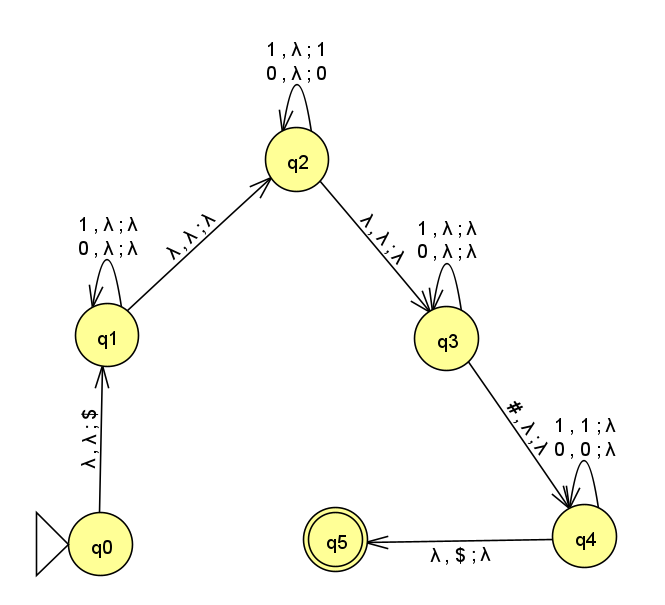
\includegraphics[scale=0.5]{assets/pda_3.png}
        \end{center}
    \end{mdframed}
\end{enumerate}

\subsection{Conventions for PDAs}
\begin{itemize}
    \item We can \emph{test for the end of the stack}, without providing details. We can always push the end-of-stack symbol \code{\$} at the start. 
    \item We can \emph{test for the end of the input} without providing details. We can transform the PDA to one where accepting states are only those reachable when there are no more input symbols. 
    \item We don't always need to provide a state transition diagram.
\end{itemize}









































\newpage 
\section{Turing Machines (3.1)}
First proposed by Alan Turing in 1936, the \textbf{Turing machine} is a much more accurate model of a general purpose computer. It can do everything that a real computer can do, but even it cannot solve certain problems\footnote{In a very real sense, these problems are beyond the theoretical limits of computation.}.

\subsection{The Idea}
\begin{itemize}
    \item The input string is \emph{written} on the leftmost squares of the tape. The rest of the tape is empty. 
    \item We can read \emph{and} write on the tape. The read/write head starts at the leftmost position on the tape. 
    \item Computation proceeds according to the transition function. In other words, given the current state of machine, and the current symbol being read, the machine will 
    \begin{itemize}
        \item Transition to a new state.
        \item Write a symbol to its current position, overwriting the existing symbol.
        \item Moves the tape head $L$ or $R$. 
    \end{itemize}
    \item Computation ends if and when it enters either the \textbf{accept} or the \textbf{reject} state. This means that we can have programs that can run forever. 
\end{itemize}

\subsection{Language of a Turing Machine}
Given a Turing machine $M$, the language $L(M)$ is the set of all strings $w$ such that the computation of $M$ on $w$ \emph{halts} after entering the accept state. That is, $L(M) = \{w \mid w \text{ is accepted by } M\}$.

\subsection{Formal Definition}
As usual, the most important thing about the Turing machine is the transition function 
\[\delta: Q \times \Gamma \mapsto Q \times \Gamma \times \{L, R\}\]
That is, when the machine is in a certain state $q$ and the head is over a tape square containing the symbol $a$, and if $\delta(q, a) = (r, b, L)$, then the machine writes the symbol $b$ replacing the $a$, and goes to state $r$. The third component is either $L$ or $R$, and indicates whether the head moves to the left or right after writing. In this case, the $L$ indicates that we move the tape to the left. 

\begin{definition}{Turing Machine}{}
    A \textbf{Turing machine} is a 7-tuple $(Q, \Sigma, \Gamma, \delta, q_0, q_{\text{accept}}, q_{\text{reject}})$ where $Q, \Sigma, \Gamma$ are all finite sets and 
    \begin{enumerate}
        \item $Q$ is the set of states.
        \item $\Sigma$ is the input alphabet not containing the \emph{blank symbol} $\sqcup$.
        \item $\Gamma$ is the tape alphabet, where $\sqcup \in \Gamma$ and $\Sigma \subseteq \Gamma$. 
        \item $\delta: Q \times \Gamma \mapsto Q \times \Gamma \times \{L, R\}$ is the transition function. 
        \item $q_0 \in Q$ is the start state. 
        \item $q_{\text{accept}} \in Q$ is the accept state.
        \item $q_{\text{reject}} \in Q$ is the reject state, where $q_{\text{reject}} \neq q_{\text{accept}}$.   
    \end{enumerate} 
\end{definition}

\subsection{Configuration of a Turing Machine}
As a Turing machine computes, changes occur in the current state, the current tape contents, and the current head location. A setting of these three items is called a \textbf{configuration} of the Turing machine. They are often represented in a special way. For a state $q$ and two strings $u$ and $v$ over the tape alphabet $\Gamma$, we write $uqv$ for the configuration where the current state is $q$, the current tape contents is $uv$, and the current head location is the first symbol of $v$. 

\bigskip 

For example, $\code{1011}q_7\code{01111}$ represents the configuration when the tape is \code{101101111}, the current state is $q_7$, and the head is currently on the second \code{0}.
\begin{center}
    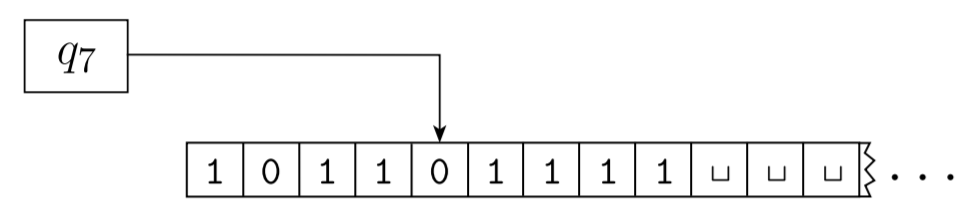
\includegraphics[scale=0.5]{assets/turing_config_1.png}

    \textbf{Figure:} The configuration $\code{1011}q_7\code{01111}$. 
\end{center}

\subsubsection{Transitioning Between Configurations}
Suppose that a configuration $C_1$ \textbf{yields} configuration $C_2$ if the Turing machine can legally go from $C_1$ to $C_2$ in a single step. We can define this notion formally as follows: suppose we have $a, b, c \in \Gamma$, as well as $u, v \in \Gamma^*$ and states $q_i, q_j \in Q$. In that case, $ua q_i bv$ and $uq_j acv$ are two arbitrary configurations. Say that 
\[uaq_i bv \text{ yields } uq_j acv\]
if, in the transition function, $\delta(q_i, b) = (q_j, c, L)$. This handles the case where the Turing machine moves leftward. For a rightward move, say that 
\[uaq_i bv \text{ yields } uacq_j v\]
if, in the transition function, $\delta(q_i, b) = (q_j, c, R)$. 

\subsubsection{Start, Accepting, Rejecting, and Halting Configurations}
The start configuration of $M$ on input $w$ is the configuration $q_0 w$, which indicates that the machine is in the start state $q_0$ with its head at the leftmost position on the tape.

\bigskip 

In an accepting configuration, the state of the configuration is $q_{\text{accept}}$.

\bigskip 

In a rejecting configuration, the state of the configuration is $q_{\text{reject}}$.

\bigskip 

Accepting and rejecting configurations are halting configurations and do not yield further configurations. 

\subsection{Deciders and Recognizers}
We now briefly talk about the difference between deciders and recognizers. 

\subsubsection{Turing-Recognizable}
A language is \textbf{Turing-recognizable} if some Turing machine recognizes it, i.e. if $L = L(M)$ for some Turing machine $M$. When we start a Turing machine on some input, the machine can either \emph{accept}, \emph{reject}, or \emph{loop}. However, sometimes we don't want the machine to loop. 

\subsubsection{Turing-Decider}
A Turing machine $M$ is a \textbf{decider} Turing machine (either Turing-decidable or decidable) if it halts on all inputs (i.e. never loops). 

\bigskip 

$L$ is \textbf{Turing-decidable} if some Turing machine that is a decider recognizes it. 


\subsubsection{Example 1: Turing Machine}
Consider the language $L = \{w\code{\#}w \mid w \in \{\code{0}, \code{1}\}^*\}$, which is both not regular and not context-free. 

\begin{enumerate}
    \item Give an idea for a potential Turing machine that recognizes $L$.

    \begin{mdframed}[]
        The idea is as follows
        \begin{itemize}
            \item We want to zig-zag across tapes to corresponding positions on either side of \code{\#} to check whether these positions agree. If they do not, or there is no \code{\#}, then we reject. If they do, then cross them off. 
            \item Once all symbols to the left of the \code{\#} are crossed off, check for any symbols to the right of \code{\#}. If there are any, \emph{reject}. Otherwise, accept.
        \end{itemize}
        To see what we mean, consider the following example  
        \begin{verbatim}
            0 1 # 0 1
            -> x 1 # 0 1
               ^
            -> x 1 # x 1
                     ^ 
            -> x x # x 1
                 ^ 
            -> x x # x x
                       ^
        \end{verbatim}
    \end{mdframed}

    \item Is this machine a decider? 
    \begin{mdframed}[]
        Yes, because it will halt (either accept or reject) no matter what the input is. 
    \end{mdframed}

    \item Draw the state diagram corresponding to the Turing machine. 
    \begin{mdframed}[nobreak=true]
        \begin{center}
            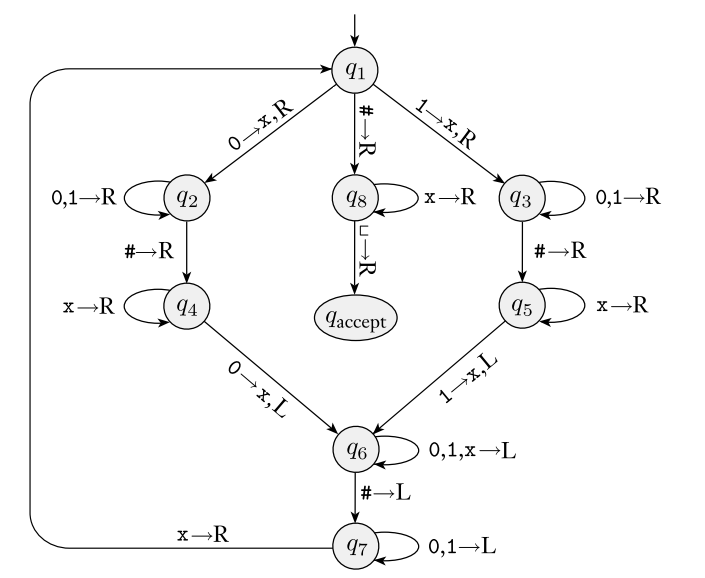
\includegraphics[scale=0.7]{assets/turing_1.png}
        \end{center}

        To simplify the figure, we don't show the reject state or the transitions going to the reject state. Those transitions occur implicitly whenever a state lacks an outgoing transition for a particular symbol.
    \end{mdframed}

    \item What is $Q$ (the set of states)?
    \begin{mdframed}[]
        \[Q = \{q_1, \dots, q_8, q_{\text{accept}}, q_{\text{reject}}\}\]
    \end{mdframed}

    \item What is $\Sigma$?
    \begin{mdframed}[]
        \[\Sigma = \{\code{0}, \code{1}, \code{\#}\}\]
    \end{mdframed}

    \item What is $\Gamma$?
    \begin{mdframed}[]
        \[\Gamma = \Sigma \cup \{\code{b}, \code{x}\}\]
    \end{mdframed}

    \item Given the string \code{01\#01}, run through the Turing machine. 
    \begin{mdframed}[]
        We begin with the initial configuration. 
        \begin{verbatim}
            State:      q1
            Tape:       0 1 # 0 1
              (Next:)   ^
            Config:     q1 0 1 # 0 1
        \end{verbatim}

        Here, we read in the \code{0} and move to $q_2$, replacing \code{0} with \code{x} and moving the tape to the right. 
        \begin{verbatim}
            State:      q2
            Tape:       x 1 # 0 1
              (Next:)     ^
            Config:     x q2 1 # 0 1
        \end{verbatim}

        At this point, we read in the \code{1} as well (without crossing anything out) and move the tape to the right.  
        \begin{verbatim}
            State:      q2
            Tape:       x 1 # 0 1
              (Next:)       ^
            Config:     x 1 q2 # 0 1
        \end{verbatim}

        For the same reason as above, we read in \code{\#} as well, transitioning to $q_4$ and moving the tape to the right.
        \begin{verbatim}
            State:      q4
            Tape:       x 1 # 0 1
              (Next:)         ^
            Config:     x 1 # q4 0 1
        \end{verbatim}

        Now, we read in the \code{0}, replacing it with a \code{x} and moving the tape left. We also transition to $q_6$. 
        \begin{verbatim}
            State:      q6
            Tape:       x 1 # x 1
              (Next:)       ^
            Config:     x 1 q6 # x 1
        \end{verbatim}

        We read in the \code{\#}, moving the tape to the left and transitioning to $q_7$. 
        \begin{verbatim}
            State:      q7
            Tape:       x 1 # x 1
              (Next:)     ^
            Config:     x q7 1 # x 1
        \end{verbatim}

        We now keep looping at $q_7$ whenever we see a \code{0} or \code{1}. In our case, we only need to read one \code{1}, so we do that, while also moving the tape to the left. 
        \begin{verbatim}
            State:      q7
            Tape:       x 1 # x 1
              (Next:)   ^
            Config:     q7 x 1 # x 1
        \end{verbatim}

        We now read in the \code{x} and transition to $q_1$, moving the tape to the right. 
        \begin{verbatim}
            State:      q1
            Tape:       x 1 # x 1
              (Next:)     ^
            Config:     x q1 1 # x 1
        \end{verbatim}

        Now, we transition to $q_3$, reading in the \code{1} and replacing it with an \code{x} while also moving the tape to the right. 
        \begin{verbatim}
            State:      q3
            Tape:       x x # x 1
              (Next:)       ^
            Config:     x x q3 # x 1
        \end{verbatim}

        We now read in the \code{\#}, moving the tape to the right and transitioning to $q_5$.
        \begin{verbatim}
            State:      q5
            Tape:       x x # x 1
              (Next:)         ^
            Config:     x x # q5 x 1
        \end{verbatim}

        We now read in all of the \code{x}'s, moving the tape to the right. We only do this once as there is only one \code{x} to be read. 
        \begin{verbatim}
            State:      q5
            Tape:       x x # x 1
              (Next:)           ^
            Config:     x x # x q5 1
        \end{verbatim}

        We now read in a \code{1}, replacing it with a \code{x}, transitioning to $q_6$, and moving the tape to the left. 
        \begin{verbatim}
            State:      q6
            Tape:       x x # x x
              (Next:)         ^
            Config:     x x # q6 x x
        \end{verbatim}

        At $q_6$, we keep reading in the \code{x}'s. We only do this once, so we move the tape one to the left. 
        \begin{verbatim}
            State:      q6
            Tape:       x x # x x
              (Next:)       ^
            Config:     x x q6 # x x
        \end{verbatim}

        Now, we transition to $q_7$ since the next symbol is \code{\#}, moving the tape to the left. 
        \begin{verbatim}
            State:      q7
            Tape:       x x # x x
              (Next:)     ^
            Config:     x q7 x # x x
        \end{verbatim}

        We transition to $q_1$, moving the tape to the right. 
        \begin{verbatim}
            State:      q1
            Tape:       x x # x x
              (Next:)       ^
            Config:     x x q1 # x x
        \end{verbatim}

        Since the next symbol to be read is a \code{\#}, we transition to $q_8$, moving the tape to the right. 
        \begin{verbatim}
            State:      q8
            Tape:       x x # x x
              (Next:)         ^
            Config:     x x # q8 x x
        \end{verbatim}

        We now keep reading in any \code{x}'s, moving the tape to the right. This is done twice.
        \begin{verbatim}
            State:      q8
            Tape:       x x # x x
              (Next:)             ^
            Config:     x x # x x q8
        \end{verbatim}

        At this point, we are implicitly at a $\sqcup$. So, we move to $q_{\text{accept}}$. Thus, this string is accepted.
    \end{mdframed}
\end{enumerate}

\subsection{Describing Turing Machines}
There are several ways we can describe Turing machines. 
\begin{itemize}
    \item \textbf{Formal Definition:} A set of states, input alphabet, tape alphabet, transition function, start state, accept state, and reject state. Essentially, drawing out the Turing machine. This is the most detailed level of description. 
    \item \textbf{Implementation-Level Definition:} English prose to describe Turing machine head movements relative to the contents of the tape; in other words, we use English prose to describe the way that the Turing machine moves its head and the way that it stores data on its tape. Note that we do not give details of states or transition function.
    \item \textbf{High-Level Description:} A description of the algorithm, without the implementation details of a machine. As part of this description, we can ``call'' and run another Turing machine as a subroutine. Here, we do not need to mention how the machine manages its tape or head.
\end{itemize}

\subsubsection{Example: Describing Turing Machines}
Give an \emph{implementation-level} description of a Turing machine which \emph{decides} the empty set. 

\begin{mdframed}[]
    Let $M$ be the Turing machine where, on some input $w$, we reject.
\end{mdframed}

\subsubsection{Example: Describing Turing Machines}
Give a \emph{high-level} description of a Turing machine which \emph{decides} the language 
\[A = \{\cyclic{G} \mid G \text{ is a connected undirected graph}\}\]
Here, we say that $\cyclic{G}$ is the encoding of the graph. For example, if $G$ is defined by 
\[G = (V, E)\]
where 
\[V = \{1, 2, 3, 4\} \qquad E = \{(1, 2), (2, 3), (3, 1), (1, 4)\}\]
then the encoding is given by 
\[\cyclic{G} = \code{(1,2,3,4)((1,2),(2,3),(3,1),(1,4))}\]

\begin{mdframed}[]
    Let $M$ be the Turing machine where, on input $\cyclic{G}$ (the encoding of the graph), we do the following: 
    \begin{enumerate}
        \item Select the first node of $G$ and mark it. 
        \item While we still have nodes to mark, for each node in $G$, mark it if it is attached by an edge to a node that is already marked. 
        \item Scan all the nodes of $G$ to determine whether they are all marked. If they are, \emph{accept}. Otherwise, \emph{reject}.
    \end{enumerate}
\end{mdframed}


\subsection{Class of Recognizable and Decidable Languages}
The class of decidable \emph{and} recognizable languages is closed under:
\begin{itemize}
    \item Union. 
    \item Concatenation. 
    \item Intersection. 
    \item Kleene Star. 
\end{itemize}
The class of \emph{decidable} languages is also closed under complementation. 

\subsubsection{Class of Decidable Languages Closed Under Union}
\begin{theorem}{}{}
    The class of decidable languages over a fixed alphabet $\Sigma$ is closed under union. 
\end{theorem}

\begin{mdframed}[nobreak=true]
    \begin{proof}
        Let $L_1$ and $l_2$ be languages over $\Sigma$ and suppose $M_1$ and $M_2$ are Turing machines that decide these languages, respectively. We will define a new Turing machine, $M$, via a high-level description. For some input $w$, the Turing machine $M$ will do the following: 
        \begin{enumerate}
            \item Run $M_1$ on input $w$. If $M_1$ accepts $w$, then accept. Otherwise, go to the next step. 
            \item Run $M_2$ on input $w$. If $M_2$ accepts $w$, then accept. Otherwise, we reject. 
        \end{enumerate} 
        To show correctness, we need to show that $L(M) = L_1 \cup L_2$ and that $M$ is a decider. For some string $s$, if $L_1$ or $L_2$ contains $s$, then clearly the machine must recognize it. We know this is the case because our machine runs $M_1$ and then runs $M_2$ if $M_1$ doesn't yield an \emph{accept} state. Now, if $M_1$ and $M_2$ both reject, then clearly $s$ must not be in any of the two languages, and will thus not be in $M$. To show that $M$ is a decider, we note that $M$ will either accept (if $s$ is accepted by any of the two machines) or reject if both $M_1$ and $M_2$ reject. So, there's no chance that it will loop.  
    \end{proof}
\end{mdframed}









































\newpage 
\section{Variants of Turing Machines (3.2)}
There are, of course, different variations of Turing machines. Some of these variants may have multiple tapes, or may use nondeterminism. The original Turing machine and its variants all have the same power in the sense that they recognize the same class of languages. 

\subsection{Multitape Turing Machine}
A \textbf{multitape Turing machine} is like an ordinary Turing machine with several tapes. Each tape has its own head for reading and writing. Initially, the input appears on the first tape, and the other tapes start out blank. In order to accomodate for the fact that there are multiple tapes, we now introduce a new transition function which allows for reading, writing, and moving the heads on some or all of the tapes simultaneously:
\[\delta: Q \times \Gamma^k \mapsto Q \times \Gamma^k \times \{L, R, S\}^k\]
where $k$ is the number of tapes. So, it follows that the expression 
\[\delta(q_i, a_1, \dots, a_k) = (q_j, b_1, \dots, b_k, L, R, \dots, L)\]
means that if the machine is in state $q_i$ and heads 1 through $k$ are reading the symbols $a_1$ through $a_k$, the machine goes to state $q_j$ and writes symbols $b_1$ through $b_k$, and directs each head to move left or right (or stay put, $S$), as specified. 

\subsubsection{Multitape vs. Single-tape Turing Machines}
\begin{theorem}{}{}
    Every multitape Turing machine has an equivalent single-tape Turing machine.
\end{theorem}
\textbf{Remark:} This is Theorem 3.13 in the textbook. The proof can be found there. 

\begin{mdframed}[]
    (Idea.) To show equivalence, we need to do the following: 
    \begin{itemize}
        \item Given a Turing machine, we can build a multitape Turing machine which recognizes the same language. 
        \item Given a $k$-tape Turing machine, we can build a one-tape Turing machine recognizing the same language. 
    \end{itemize}
    To do this, we can make use of a delimiter to keep tape contents separate, and then use a special symbol to indicate the location of each read/write head. 
\end{mdframed}

\subsubsection{Turing-Recognizability}
\begin{corollary}{}{}
    A language is Turing-recognizable if and only if some multitape Turing machine recognizes it.
\end{corollary}

\begin{mdframed}[]
    \begin{proof}
        A Turing-recognizable language is recognized by an ordinary (single-tape) Turing machine, which is a special case of a multitape Turing machine. This proves one direction of the corollary. The other direction comes as part of the proof of the above theorem. 
    \end{proof}
\end{mdframed}

\subsection{Nondeterministic Turing Machines}
A \textbf{nondeterministic Turing machine} is defined in the expected way. At any point in a computation, the machine can proceed according to several possibilities. The transition function, then, has the form 
\[\delta: Q \times \Gamma \mapsto \PowerSet(Q \times \Gamma \times \{L, R\})\]
Like a nondeterministic finite automaton, if a computation ends up at an accept state, then the machine as a whole accepts the input. If, after going through all possibilities, the machine doesn't reach an accept state, then the machine rejects the input.  

\subsubsection{Nondeterministic vs. Deterministic Turing Machines}
\begin{theorem}{}{}
    Every nondeterministic Turing machine has an equivalent deterministic Turing machine. 
\end{theorem}

\begin{mdframed}[]
    \begin{proof}
        (Idea.) For the proof of equivalence, we need to show two things. 
        \begin{enumerate}
            \item Given a Turing machine, we need to build a nondeterminism Turing machine recognizing the same language. 
            \item Given a nondeterminism Turing machine, we need to build a deterministic Turing machine recognizing the same language. 
        \end{enumerate}
        To do this, we can try all possible branches of the nondeterministic computation. We have three tapes: a ``read-only'' input tape, a simulation tape, and a tape tracking nondeterminism branching. 
    \end{proof}
\end{mdframed}

\subsubsection{Turing-Recognizability}
\begin{corollary}{}{}
    A language is Turing-recognizable if and only if some nondeterministic Turing machine recognizes it. 
\end{corollary}

\begin{mdframed}[]
    \begin{proof}
        Any deterministic Turing machine is automatically a nondeterministic Turing machine, so one direction of the corollary follows immediately. For the other direction, we can consider the proof of the theorem above. 
    \end{proof}
\end{mdframed}

\subsubsection{Turing-Decidable}
The proof of the theorem can be modifier so that if the nondeterministic Turing machine always halts on all branches of its computation, then its corresponding deterministic Turing mahcine will as well. 
\begin{corollary}{}{}
    A language is decidable if and only if some nondeterministic Turing machine recognizes it. 
\end{corollary}


\subsection{Enumerators}
Loosely defined, an enumerator is a Turing machine with an attached printer. Then, the Turing machine can use that printer as an output device to print strings out. Every time the Turing machine wants to ad a string to the list, it sends that string to the printer. 

\bigskip 

An enumerator $E$ starts with a blank tape on its work tape. Now, if the enumerator doesn't half, then it may print an infinite list of strings. The language enumerated by $E$ is the collection of all the strings that it will eventually print out. Moreover, $E$ may generate the strings of the langauge in \emph{any order}, possibly \emph{with repetition}.

\bigskip 

For any given $\Sigma$, there is an enumerator whose language is the set of all strings over $\Sigma$. To see this, we do standard string ordering. In particular: 
\begin{itemize}
    \item Order strings first by length. 
    \item Then, by dictionary order. 
\end{itemize}

\subsubsection{Turing-Recognizability}
\begin{theorem}{}{}
    A language is Turing-recognizable if and only if some enumerator enumerates it. 
\end{theorem}

\begin{mdframed}[]
    \begin{proof}
        First, we want to show that if we have an enumerator $E$ that enumerates a language $A$, then a Turing machine $A$ recognizes $A$. To describe $M$, we note that on some input $w$, we: 
        \begin{enumerate}
            \item Run $E$. Every time that $E$ outputs a string, compare it with $w$. 
            \item If $w$ ever appears in the output of $E$, accept it. 
        \end{enumerate}
        Clearly, $M$ accepts those strings that appear on $E$'s list. To show the other direction, note that if a Turing machine $M$ recognizes a language $A$, then we can construct the following enumerator $E$ for $A$. Say that $s_1, s_2, s_3 \dots$ is a list of all possible strings in $\Sigma^*$. Then, for some input $w$, we can describe $E$ like so:
        \begin{enumerate}
            \item Ignore the input. 
            \item Repeat the following for $i = 1, 2, 3, \dots$: 
            \begin{itemize}
                \item Run $M$ for $i$ steps on each input $s_1, s_2, \dots, s_i$. 
                \item If any computations accept, print out the corresponding $s_j$.
            \end{itemize}
        \end{enumerate}
        If $M$ accepts a particular string $w$, then it will eventually appear on the list generated by $E$. In fact, it will appear on the list infinitely many times because $M$ runs from the beginning on each string for each repetition of step 1. This procedures gives the effect of running $M$ in parallel on all possible input strings. 
    \end{proof}
\end{mdframed}


\subsection{Summary}
Suppose $M$ is a Turing machine and $E$ is an enumerator. Suppose that $L$ is a language and $w$ is a string.
\begin{center}
    \begin{tabular}{p{0.5in}|p{1.5in}|p{1.5in}|p{1.5in}}
            & $M$ Recognizes $L$ & $M$ Decides $L$ & $E$ Enumerates $L$ \\ 
        \hline 
        $w \in L$ & Accept & Accept. & Prints $w$ at some point. \\ 
        $w \notin L$ & Reject or Loop. & Reject. & Never prints $w$. 
    \end{tabular}
\end{center}





\newpage
\section{Decidability (4.1)} 
In this section we give some examples of languages that are decidable by algorithms. 

\bigskip 

A computational problem is \textbf{decidable} if and only if the language encoding the problem instances is decidable. 

\subsection{Encoding Inputs}
First, we should mention that not all inputs are strings. In past examples and problems, we've generally worked with strings in a set alphabet. But, what if our input is an array of integers? 

\bigskip 

By definition, all Turing machine inputs are \emph{strings}. If we're given an input that isn't a string, we need to \textbf{encode} the input (represent it as a string) first. 

\bigskip 

Before we discuss further, here is some notation: 
\begin{itemize}
    \item $\cyclic{O}$ is the string that represents, or encodes, the object $O$ ($O$ could be, for example, an integer, an array, etc.)
    \item $\cyclic{O_1, O_2, \dots, O_n}$ is the single string that represents the tuple of objects $O_1, O_2, \dots, O_n$. 
\end{itemize}

In this way, problems that we care about can be reframed as languages of strings. 

\subsubsection{Example: Encoding Inputs}
\begin{itemize}
    \item Recognizes whether a string is a palindrome. 
    \[\{w \mid w \in \{0, 1\}^* \text{ and } w = w^R\}\]
    No encoding is necessary since $w$ is a bitstring. 

    \item Check whether a string is accepted by a DFA. 
    \[\{\cyclic{B, w} \mid B \text{ is a DFA over } \Sigma, w \in \Sigma^*, w \in L(B)\}\]
    Here, we encode the pair $B$ and $w$, where 
    \begin{itemize}
        \item $B$ is a DFA. 
        \item $w$ is a string. 
    \end{itemize}
    Essentially, for this language, saying that it's decidable is equivalent to checking if the string is accepted by the DFA. 

    \bigskip 

    As a more general example, suppose we have a JSON file describing a DFA and a string. Then, we want to create an algorithm that checks whether this string is accepted by this DFA. 

    \item Check whether the language of a PDA is infinite.
    \[\{\cyclic{A} \mid A \text{ is a PDA and } L(A) \text{ is infinite}\}\]
    Here, $A$ is an encoding of a PDA. 
\end{itemize}

\subsection{Computational Problems}
We now go over some example computational problems that are decidable.

\subsubsection{Example: Recognizing Input Strings}
Consider, again, the following language 
\[A_{\text{DFA}} = \{\cyclic{B, w} \mid B \text{ is a DFA that accepts input string } w\}\]
This language contains the encodings of all DFAs together with strings that the DFAs accept. Then, the problem of testing whether the DFA $B$ accepts an input $w$ is the same as the problem of testing whether $\cyclic{B, w} \in A_{\text{DFA}}$. 

\begin{theorem}{}{}
    $A_{\text{DFA}}$ is a decidable language. 
\end{theorem}

\begin{mdframed}[]
    \begin{proof}
        (Idea.) We simply need to present a Turing machine $M$ that decides $A_{\text{DFA}}$. Let $M$ be the Turing machine which takes in an input $\cyclic{B, w}$, where $B$ is a DFA and $w$ is a string, and does the following: 
        \begin{enumerate}
            \item Simulate $B$ on input $w$ (by keeping track of states in $B$, the transition function of $B$, etc.)\footnote{It's like writing a program that simulates the DFA.}
            \item If the simulation ends in an accept state, then accept. If it ends in a nonaccepting state, then reject. 
        \end{enumerate}
        A reasonable implementation of $B$ is simply a list of its five components, $Q$, $\Sigma$, $\delta$, $q_0$, and $F$. Then, when $M$ receives its input, $M$ first determines whether it properly represents a DFA $B$ and a string $w$. If not, $M$ rejects. Otherwise, $M$ carries out the simulation directly; it keeps track of $B$'s current state and $B$'s current position in the input $w$ by writing this information to its tape. Initially, $B$'s current state is $q_0$, and $B$'s current input position is the leftmost symbol of $w$. The states and position are updated according to the specified transition function $\delta$. When $M$ finishes processing the last symbol of $w$, it checks whether $B$ is in an accept state. If so, $M$ accepts. Otherwise, $M$ rejects.
    \end{proof}
\end{mdframed}

\subsubsection{Example: Emptiness Test}
Consider the following language
\[E_{\text{DFA}} = \{\cyclic{A} \mid A \text{ is a DFA and } L(A) = \emptyset\}\]
Here, we want to determine whether a finite automaton accepts any strings at all. 

\begin{theorem}{}{}
    $E_{\text{DFA}}$ is a decidable language.
\end{theorem}

\begin{mdframed}[]
    \begin{proof}
        A DFA accepts some string if and only if reaching an accept state from the start state by traveling along the arrows of the DFA is possible. To test this condition, we can design a TM $T$ that uses a marking algorithm similar to what we used in the previous sections. For an input $A$, where $A$ is a DFA, we describe the TM $T$ as follows:
        \begin{enumerate}
            \item Check whether $A$ is a valid encoding of a DFA; if not, reject. 
            \item Mark the start state of $A$. 
            \item Repeat until no new states get marked: 
            \begin{itemize}
                \item Loop over states of $A$ and mark any unmarked state that has an \textbf{incoming} edge from a marked state. 
            \end{itemize}
            \item If no accept state is marked, \emph{accept}. Otherwise, \emph{reject}.
        \end{enumerate}
        This concludes the proof. 
    \end{proof}
\end{mdframed}

\subsubsection{Example: Equivalent DFAs}
Consider the following language
\[EQ_{\text{DFA}} = \{\cyclic{A, B} \mid A \text{ and } B \text{ are DFAs and } L(A) = L(B)\}\]
Here, this language contains the encodings of all equivalent DFAs. 

\begin{theorem}{}{}
    $EQ_{\text{DFA}}$ is a decidable language.
\end{theorem}

\begin{mdframed}[]
    \begin{proof}
        To prove this theorem, we make use of the previous theorem. We construct a DFA $C$ from $A$ and $B$, where $C$ accepts only those strings that are accepted by either $A$ and $B$ but \emph{not} by both. Thus, if $A$ and $B$ recognize the same language, then $C$ will accept nothing. Recall that, for two sets $X$ and $Y$: 
        \[X = Y \iff \left(X \cap \overline{Y}\right) \cup \left(Y \cap \overline{X}\right) = \emptyset\]
        Using this as inspiration, the language of $C$ is then given by: 
        \[L(C) = \left(L(A) \cap \overline{L(B)}\right) \cup \left(\overline{L(A)} \cap L(B)\right)\]
        This expression is sometimes called the \textbf{symmetric difference} of $L(A)$ and $L(B)$. Then, we can build a new DFA that recognizes the symmetric difference of $A$ and $B$. Then, we can check if this set is empty by using the example from the previous section. If so, then we \emph{accept}. Otherwise, we \emph{reject}.

        \bigskip 

        The construction of this Turing machine is as follows; define a Turing machine $M_3$ that takes in the input $\cyclic{A, B}$ and does the following: 
        \begin{enumerate}
            \item Check whether $A$ and $B$ are valid encodings of DFAs; if not, reject.
            \item Construct a new DFA, $D$, from $A$ and $B$ using the algorithms for complementing and taking union of regular languages such that 
            \[L(D) = \text{Symmetric difference of } A \text{ and } B\]
            \item Run the machine from the previous example on $D$. 
            \item If the machine from the previous example accepts, then accept. If it rejects, then reject. 
        \end{enumerate}
        Therefore, we are done. 
    \end{proof}
\end{mdframed}


\subsubsection{Example: Regular Expressions and DFAs}
Consider the following language 
\[L = \{\cyclic{R, D} \mid R \text{ is a regular expression, } D \text{ is a DFA, and } L(R) = L(D)\}\]
We now show that this language is decidable. 
\begin{mdframed}[]
    \begin{proof}
        (Idea.) To show that this language is decidable, we construct a Turing machine. For input $\cyclic{R, D}$, where $R$ is some arbitrary regular expression and $D$ is some arbitrary DFA, the Turing machine $M_4$ will do the following: 
        \begin{enumerate}
            \item Convert $R$ to a DFA $D_R$. 
            \item Check if $L(D_R) = L(D)$. 
            \begin{itemize}
                \item We have reduced this problem to $EQ_{\text{DFA}}$. 
                \item Note that $EQ_{\text{DFA}}$ is decidable as $EQ_{\text{DFA}}$ depends on $E_{\text{DFA}}$ and $E_{\text{DFA}}$ is decidable. 
                \item Since $E_{\text{DFA}}$ is decidable, we can check the symmetric difference of $D_R$ and $D$ and see if it is empty by using $E_{\text{DFA}}$. 
            \end{itemize}
        \end{enumerate}
        Therefore, $L$ is decidable. 
    \end{proof}
\end{mdframed}

\subsubsection{Example: 10 Steps in a Turing Machine}
Consider the following language 
\[L = \{\cyclic{M, w} \mid M \text{ is a Turing machine which runs for at least 10 steps on input } w\}\]
We now show that this langauge is decidable.
\begin{mdframed}[]
    \begin{proof}
        (Idea.) Run $M$ on $w$ for 9 steps. If $M$ accepts or rejects after at most 9 steps, then we can reject (as the machine didn't run at least 10 steps). Otherwise, accept. 
    \end{proof}
\end{mdframed}

\subsection{Techniques}
The techniques we have discussed are as follows: 
\begin{itemize}
    \item \textbf{Subroutines:} We can use decision procedures of decidable problems as subroutines in other algorithms. 
    \item \textbf{Constructions:} We can use algorithms for constructions as subroutines in other algorithms.
    \begin{itemize}
        \item Converting DFA to DFA recognizing complement or Kleene star. 
        \item Converting two DFAs/NFAs to one recognizing union, intersection, concatenation. 
        \item Converting NFA to equivalent DFA. 
        \item Converting regular expression to equivalent NFA. 
        \item Converting DFA to equivalent regular expression.
    \end{itemize}
\end{itemize}









































\newpage 
\section{Undecidability (4.2)} 
We will now talk about several computationally unsolvable problems, along with proving that such problems are actually unsolvable.

\subsection{Computational Problems}
We begin by going over some examples of computational problems. 

\subsubsection{Simple Problems: DFAs}
Recall the following examples from the previous notes. 
\begin{itemize}
    \item Check whether a string is accepted by a DFA. 
    \[A_{\text{DFA}} = \{\cyclic{B, w} \mid B \text{ is a DFA over } \Sigma, w \in \Sigma^*, w \in L(B)\}\]

    \item Check whether the language of a DFA is empty. 
    \[E_{\text{DFA}} = \{\cyclic{A} \mid A \text{ is a DFA and } L(A) = \emptyset\}\]
    
    \item Check whether the languages of two DFAs are equal.
    \[EQ_{\text{DFA}} = \{\cyclic{A, B} \mid A \text{ and } B \text{ are DFAs and } L(A) = L(B)\}\]
\end{itemize}
These are \textbf{all} decidable; we did this by constructing algorithms that could solve them. 

\subsubsection{More Complex Problems: Pushdown Automaton}
Consider the following examples.
\begin{itemize}
    \item Check whether a string is accepted by a PDA. 
    \[A_{\text{PDA}} = \{\cyclic{B, w} \mid B \text{ is a PDA over } \Sigma, w \in \Sigma^*, w \in L(B)\}\]

    \item Check whether the language of a PDA is empty. 
    \[E_{\text{PDA}} = \{\cyclic{A} \mid A \text{ is a PDA and } L(A) = \emptyset\}\]
    
    \item Check whether the languages of two PDAs are equal.
    \[EQ_{\text{PDA}} = \{\cyclic{A, B} \mid A \text{ and } B \text{ are PDAs and } L(A) = L(B)\}\]
\end{itemize}
Some of these are decidable, and some are not. We note that, because a PDA has a stack which can be infinite in size, we cannot just simulate a PDA with the infinite because there can be infinitely many options. 

\subsubsection{Complex Problems: Turing Machine}
Consider the following examples.
\begin{itemize}
    \item Check whether a string is accepted by a TM. 
    \[A_{\text{TM}} = \{\cyclic{B, w} \mid B \text{ is a TM over } \Sigma, w \in \Sigma^*, w \in L(B)\}\]

    \item Check whether the language of a TM is empty. 
    \[E_{\text{TM}} = \{\cyclic{A} \mid A \text{ is a TM and } L(A) = \emptyset\}\]
    
    \item Check whether the languages of two TMs are equal.
    \[EQ_{\text{TM}} = \{\cyclic{A, B} \mid A \text{ and } B \text{ are TMs and } L(A) = L(B)\}\]
\end{itemize}
These are all undecidable. There are no algorithms which can solve $A_{\text{TM}}$, for example.

\subsection{\texorpdfstring{$A_{\text{TM}}$}{Checking if TM Accepts String}: An Algorithm}
We will now consider an algorithm for solving $A_{\text{TM}}$. For an input $\cyclic{M, w}$, define the Turing machine $N$ as follows.
\begin{enumerate}
    \item Simulate $M$ on input $w$. 
    \item If $M$ ever enters its accept state, then accept; if $M$ ever enters its reject state, then reject.
\end{enumerate}
Then, we can define
\[L(N) = A_{\text{TM}}\]
and say that $N$ is a \textbf{recognizer} for $A_{\text{TM}}$. However, $N$ is not a \emph{decider} for $A_{\text{TM}}$ because it's possible that the Turing machine $M$ can \emph{loop} (i.e. not accept or reject); if $M$ loops, then so will $N$.

\subsection{Diagonalization Method}
We now talk about the diagonalization method as a way to show that $A_{\text{TM}}$ is undecidable.

\subsubsection{Proof}
\begin{mdframed}[]
    \begin{proof}
        Assume towards a contradiction that $A_{\text{TM}}$ is decidable. Then, call $M_{A_{\text{TM}}}$ the decider for $A_{\text{TM}}$. We can define $M_{A_{\text{TM}}}$ like so: 
        \begin{mdframed}[]
            (\textbf{A}.) For input $\cyclic{M, w}$, where $M$ is a Turing machine and $w$ is a string, we can define the Turing machine $M_{A_{\text{TM}}}$ like so:
            \begin{itemize}
                \item If $w$ is in $L(M)$, i.e. if $M$ accepts $w$, then halt and \emph{accept}.
                \item If $w$ is not in $L(M)$, i.e. if $M$ rejects $w$, then halt and \emph{reject}. 
            \end{itemize}
        \end{mdframed}
        Next, we can construct a new Turing machine $D$, which uses $M_{A_\text{TM}}$ as a subroutine: 
        \begin{mdframed}[]
            (\textbf{B}.) For some input $\cyclic{M}$, we can define the Turing machine $D$ as follows:
            \begin{itemize}
                \item Run $M_{A_{\text{TM}}}$ on $\cyclic{M, \cyclic{M}}$ (here, $w = \cyclic{M}$). 
                \item If $M_{A_{\text{TM}}}$ (in the previous step) accepts, then $D$ rejects. Likewise, if $M_{A_{\text{TM}}}$ (in the previous step) rejects, then $D$ accepts.
            \end{itemize}
        \end{mdframed}
        Now, suppose we run $D$ on input $\cyclic{D}$. Because $D$ is a decider, then either the computation halts and accepts, or the computation halts and rejects. Now: 
        \begin{itemize}
            \item If $D(\cyclic{D})$ accepts, then $M_{A_{\text{TM}}}$ with $\cyclic{D, \cyclic{D}}$ rejects\footnote{by the first step implying the second step of \textbf{B}}. But, we note that $M_{A_{\text{TM}}}$ with $\cyclic{D, \cyclic{D}}$ rejects if $D$ rejects $\cyclic{D}$\footnote{by the second step of \textbf{A}}. So, it follows that $D(\cyclic{D})$ rejects. 
            \item If $D(\cyclic{D})$ rejects, then $M_{A_{\text{TM}}}$ with $\cyclic{D, \cyclic{D}}$ accepts\footnote{by the first step implying the second step of \textbf{B}}. But, we note that $M_{A_{\text{TM}}}$ with $\cyclic{D, \cyclic{D}}$ accepts if $D$ accepts $\cyclic{D}$\footnote{by the first step of \textbf{A}}. So, it follows that $D(\cyclic{D})$ accepts.  
        \end{itemize}
        This is a contradiction since $D$ cannot accept its own input and cannot reject its own input and cannot halt. 
    \end{proof}
\end{mdframed}

\subsubsection{Another Way of Seeing It}
Recall that we can list all of the Turing machines since they are countable: 
\[M_1, M_2, M_3, \dots\]
Suppose we also have a list of \emph{distinct} inputs, call them: 
\[w_1, w_2, w_3, \dots\]
We can create this two-dimensional table where $A_{i, j}$ is defined to be the cell $[i, j]$, which is the result of running $M_i$ on input $w_j$; that is, the cell will either be 1 if $w_J \in L(M_i)$ and 0 if not.  
\begin{center}
    \begin{tabular}{c|c|c|c|c}
                & $w_1$ & $w_2$ & $w_3$ & \dots \\
        \hline 
        $M_1$   &   1   &   0   &   1   & \\
        \hline 
        $M_2$   &   0   &   0   &   1   & \\
        \hline 
        $M_3$   &       &       &       & \\
        \hline 
        \vdots  &       &       &       &
    \end{tabular}
\end{center}
Note that we made up these entries. Suppose we take the opposite of the diagonals: 
\begin{center}
    \begin{tabular}{c|c|c|c|c}
                & $w_1$ & $w_2$ & $w_3$ & \dots \\
        \hline 
        $M_1$   & \textbf{0} &   0   &   1   & \\
        \hline 
        $M_2$   &   0   & \textbf{1} &   1   & \\
        \hline 
        $M_3$   &       &       &       & \\
        \hline 
        \vdots  &       &       &       &
    \end{tabular}
\end{center}

We claim that there is no Turing machine $M$ such that $M(w_j)$ accepts if and only if $A_{j, j} = 0$ for all $j$. So, if $M_1$ accepted $w_1$, then this Turing machine will reject $w_1$; if $M_2$ rejected $w_2$, then this Turing machine will accept $w_2$. 

\begin{mdframed}[]
    \begin{proof}
        We know that $M \neq M_i$ because $M(w_i) \neq M_{i}(w_i)$.
    \end{proof}
\end{mdframed}
The proof in the previous section is simply what we have here when $w_i = \cyclic{M_i}$. 

\subsection{Summary of this Algorithm}
So, we have shown that this language is not decidable. Note that this language is also recognizable. As a general fact, a language is decidable if and only if it and its complement are both recognizable. Additionally, the complement of $A_{\text{TM}}$ is unrecognizable. 









































\newpage 
\section{Reductions and the Halting Problem (5.1)}
We now begin by talking about reductions. Before we talk about reductions, consider the following statements: 
\begin{itemize}
    \item If problem $X$ is no harder than problem $Y$, and if $Y$ is easy, then $X$ must also be easy. 
    \begin{mdframed}[]
        To get the intuition behind this, suppose you have two numbers $x$ and $y$ such that $x$ is no greater than $y$; that is, $x \leq y$. Suppose $y$ is negative. Then, $x$ must also be negative (it cannot be positive). 

        \bigskip 

        The same idea holds here. If we have two problems $X$ and $Y$ such that $X$ is no harder than (or at least as easy as) $Y$ and $Y$ is easy, then $X$ cannot be harder than $Y$; $X$ has to be \emph{as easy as, or easier than,} $Y$. 
    \end{mdframed}
    \item If problem $X$ is no harder than problem $Y$, and if $X$ is hard, then $Y$ must also be hard. 
    \begin{mdframed}[]
        Again, to get the intuition behind this, suppose you have two numbers $x$ and $y$ such that $x$ is no greater than $y$; that is, $x \leq y$. Suppose $x$ is positive. Then, $y$ must also be positive (it cannot be negative). 

        \bigskip 

        The same idea holds here. If we have two problems $X$ and $Y$ such that $X$ is no harder than (or at least as easy as) $Y$ and $X$ is hard, then $Y$ cannot be easier than $X$; $Y$ has to be \emph{as hard as, or harder than,} $X$. 
    \end{mdframed}
\end{itemize}
We can now translate this to \emph{reductions} specifically, especially in terms of decidability. That is: 
\begin{itemize}
    \item If problem $X$ is no harder than problem $Y$, and if $Y$ is \textbf{decidable}, then $X$ must also be \textbf{decidable}. 
    \item If problem $X$ is no harder than problem $Y$, and if $X$ is \textbf{undecidable}, then $Y$ must also be \textbf{undecidable}. 
\end{itemize}

When we say that problem $X$ is no harder than problem $Y$, what we really mean is: given an algorithm deciding problem $Y$, we can solve problem $X$. We will use some guaranteed solution for problem $Y$ to solve problem $X$. And, so really, what we're doing is: \emph{design an algorithm that decides problem $X$, but allow it to use the subroutine that decides problem $Y$}. We also know that, if problem $X$ is undecidable, then such an algorithm that decides problem $Y$ cannot exist, a \emph{contradiction}.



\subsection{Reduction in a Nutshell}
So, when we say that problem $X$ \emph{reduces to} problem $Y$, we mean that: 
\begin{itemize}
    \item Problem $X$ is no harder than problem $Y$, which means that 
    \item Given an algorithm deciding problem $Y$, we can solve problem $X$, which means that 
    \item Given a solution for problem $Y$, we have a solution for problem $X$. 
\end{itemize}
We can think about this in relation to packages. Suppose you wanted to solve some problem $X$. You have access to a package that can solve problem $Y$. Then, you can download this package and use this package to help solve problem $X$. 


\subsubsection{More General Examples of Reduction}
Consider the following statements. 
\begin{itemize}
    \item $\Sigma^*$ reduces to $A_{\text{TM}}$.
    \begin{mdframed}[]
        This statement is \emph{true}. The problem essentially says, if you were given an algorithm to decide $A_{\text{TM}}$, then you can use that algorithm to decide $\Sigma^*$. Now, of course, you don't need to use $A_{\text{TM}}$ at all since $\Sigma^*$ is decidable. 
    \end{mdframed}
    \item $E_{\text{DFA}}$ reduces to $\emptyset$.
    \begin{mdframed}[]
        This statement is also \emph{true}. The problem is saying, if you are given an algorithm to decide $\emptyset$, then you can use that algorithm to decide $E_{\text{DFA}}$. Now, of course, you don't need to use $\emptyset$ at all since $\emptyset$ is decidable to begin with.  
    \end{mdframed}
    \item $A_{\text{TM}}$ reduces to $\{\code{aa}\}$.
    \begin{mdframed}[]
        This statement is \emph{false}. Suppose this statement is true; then, this problem is saying that if you have a way to decide $\{\code{aa}\}$, then you have a way to decide $A_{\text{TM}}$. Well, we know that $A_{\text{TM}}$ is undecidable to begin with, so the statement is entirely false. 
    \end{mdframed}
\end{itemize}
So, essentially, any decidable problem can be reduced to a decidable problem. However, no undecidable problem can be reduced to a decidable problem. 

\subsection{The Halting Problem}
Consider the \textbf{Halting problem}, defined by 
\[\text{HALT}_{\text{TM}} = \{(\cyclic{M}, w) \mid M \text{ is a TM and } M \text{ halts on input } w\}\]
We can actually make use of the fact that $A_{\text{TM}}$ is undecidable to show that $\text{HALT}_{\text{TM}}$ is undecidable.

\subsubsection{Relationship Between the Halting Problem and \texorpdfstring{$A_{\text{TM}}$}{ATM}}
To see the difference between the two problems, we note that: 
\begin{itemize}
    \item $\text{HALT}_{\text{TM}}$ is the language of all Turing machines $M$ that \emph{halt} on input $w$. In other words, $M$ only needs to accept or reject $w$.
    \item $A_{\text{TM}}$ is a language of all Turing machines $M$ that \emph{accept} $w$. 
\end{itemize}
In this sense, $A_{\text{TM}}$ is more strict than $\text{HALT}_{\text{TM}}$. Therefore, $A_{\text{TM}}$ is a subset\footnote{Note that being a subset means nothing in terms of computational complexity/decidability.} of $\text{HALT}_{\text{TM}}$.


\subsubsection{Proving that the Halting Problem is Undecidable}
For our proof, we can use the following outline. 
\begin{itemize}
    \item Suppose, by way of contradiction, that $\text{HALT}_{\text{TM}}$ is decidable. 
    \item Then, assume that we have a machine $G$ which decides $\text{HALT}_{\text{TM}}$. 
    \item Build an algorithm that uses $G$ as a subroutine that decides $A_{\text{TM}}$. 
    \item However, this is impossible. 
    \item So, $G$ cannot possibly exist and hence $\text{HALT}_{\text{TM}}$ is undecidable.
\end{itemize}
With this in mind, our proof is as follows. 
\begin{mdframed}[]
    \begin{proof}
        Suppose, by way of contradiction, that $\text{HALT}_{\text{TM}}$ is decidable. Then, assume that we have a machine $G$ which decides $\text{HALT}_{\text{TM}}$. We can construct a new Turing machine $M_{A_{\text{TM}}}$ to decide $A_{\text{TM}}$ like so: 
        \begin{mdframed}[]
            On input $\cyclic{M, w}$, where $M$ is a Turing machine and $w$ is some input, define the Turing machine $M_{A_{\text{TM}}}$ like so:
            \begin{enumerate}
                \item Run $G$ on input $\cyclic{M, w}$. 
                \item If $G$ rejects, then reject\footnote{We have this condition because it's possible that $M$ with $w$ as its input can loop. So, if $M$ with $w$ loops, then $G(\cyclic{M, w})$ will reject as $G$ is a decider. Thus, it follows that $M_{A_{\text{TM}}}$ also rejects.}. Otherwise, run $M$ on $w$ until it halts\footnote{Since, now, we've established that $M$ cannot loop.}. 
                \begin{enumerate}
                    \item If this computation accepts, then accept. 
                    \item If this computation rejects, then reject. 
                \end{enumerate}
            \end{enumerate}
        \end{mdframed}
        To show correctness, note that: 
        \begin{itemize}
            \item If $M$ with input $w$ accepts, then $G(\cyclic{M, w})$ accepts, so we run $M(w)$ which accepts, so $M_{A_{\text{TM}}}$ also accepts.
            \item If $M$ with input $w$ rejects, then $G(\cyclic{M, w})$ accepts since it at least halted, so we run $M(w)$ which rejects, so $M_{A_{\text{TM}}}$ also rejects.
        \end{itemize}
        Clearly, if $G$ decides $\text{HALT}_{\text{TM}}$, then $M_{A_\text{TM}}$ decides $A_{\text{TM}}$. But, because $A_{\text{TM}}$ is undecidable, then it follows that $\text{HALT}_{\text{TM}}$ is also undecidable. 
    \end{proof}
\end{mdframed}


\subsection{\texorpdfstring{$E_{TM}$}{ETM} is Undecidable}
Suppose we wanted to check whether the language of a TM is empty\footnote{In other words, we want to recognize codes of Turing machines that always reject or loop.}. Recall that this problem was described like so:  
\[E_{\text{TM}} = \{\cyclic{A} \mid A \text{ is a TM and } L(A) = \emptyset\}\]
We can use proof by reduction to show that this problem is undecidable. Now, to use a proof by reduction to show that $E_{\text{TM}}$ is undecidable, we need to reduce an undecidable set \emph{to} $E_{\text{TM}}$. 

\subsubsection{Proving that \texorpdfstring{$E_{TM}$}{ETM} is Undecidable}
For our proof, we can use the following outline. Our goal is to show that $A_{\text{TM}}$ reduces to $E_{\text{TM}}$. To do so, we want to show that $A_{\text{TM}}$ reduces to $E_{\text{TM}}$. 
\begin{itemize}
    \item Assume that we have a Turing machine, $R$, that decides $E_{\text{TM}}$. 
    \item Build a new Turing machine, $M_{A_{\text{TM}}}$, that decides $A_{\text{TM}}$. 
    \begin{itemize}
        \item This new Turing machine always halts.
        \item Accept an input $\cyclic{M, w}$ if and only if $w$ is in $L(M)$. 
    \end{itemize}
\end{itemize}

\subsubsection{Attempt 1: An Incorrect Proof}
Consider the following purported proof. 
\begin{mdframed}[]
    Suppose by way of contradiction that $E_{\text{TM}}$ is decidable. Then, we can build a Turing machine, $R$, that decides $E_{\text{TM}}$. We can construct a new Turing machine $M_{A_{\text{TM}}}$ that decides $A_{\text{TM}}$ like so: 
    \begin{mdframed}[]
        On input $\cyclic{M, w}$, where $M$ is a Turing machine and $w$ is an input, define the Turing machine $M_{A_{\text{TM}}}$ like so: 

        \begin{enumerate}
            \item Run $R$ on input $\cyclic{M}$. If this rejects, then reject. 
            \item If $R$ accepts, then run $M$ on input $w$. If this accepts, then accept; if this rejects, then rejects. 
        \end{enumerate}
    \end{mdframed}
    Clearly, if $R$ decides $E_{\text{TM}}$, then $M_{A_{\text{TM}}}$ decides $A_{\text{TM}}$. But, because $A_{\text{TM}}$ is undecidable, then it follows that $E_{\text{TM}}$ is also undecidable. 
\end{mdframed}
This solution \textbf{fails} when: 
\begin{enumerate}
    \item $M(w)$ loops. 
    \item $R(\cyclic{M})$ accepts. 
\end{enumerate}
Regarding the second point, the reason why is because if we run $R$ on some input $\cyclic{M}$, and if it rejects, then this implies that the language is not empty. If it accepts, then the language is empty. So, in other words, by saying that $R$ accepts, this implies that the language is empty. If the language is empty, then there is no change that $w$ can be in the language. So, by the definition of $M_{A_{\text{TM}}}$ (which is that the string $w$ must be in $L(M)$), we can reject immediately. 

\bigskip 

Now, the case that we're not sure about is when $R$ rejects. In particular, when we have $R$, we're not even considering $w$. 

\subsubsection{Attempt 2: Correct Proof}
The trick that we can do is to design a new Turing machine that ``hard-codes'' both $M$ and $w$ in it\footnote{Another way of thinking about this is, if $w$ is our input, then we're essentially just creating a new Turing machine where we hardcode $w$ into $M$.}. Thus, the correct proof is as follows: 
\begin{mdframed}[]
    \begin{proof}
        Suppose by way of contradiction that $E_{\text{TM}}$ is decidable. Then, we can build a Turing machine, $R$, that decides $E_{\text{TM}}$. We can construct a new Turing machine $M_{A_{\text{TM}}}$ that decides $A_{\text{TM}}$ like so: 
        \begin{mdframed}[]
            On input $\cyclic{M, w}$, where $M$ is a Turing machine and $w$ is an input, define the Turing machine $M_{A_{\text{TM}}}$ like so: 
    
            \begin{enumerate}
                \item First, \emph{build} the Turing machine $X$ which, on input $x$, ignores $x$ and simulates $M$ on $w$. In other words, we can think of it like:\begin{verbatim}
                    function X(x):
                        return M(w)\end{verbatim}
                \item Run $R$ on $\cyclic{X}$. If it accepts, then reject. If it rejects, then accept. 
            \end{enumerate}
        \end{mdframed}
        To show correctness, we note that: 
        \begin{itemize}
            \item If $M(w)$ accepts, then for all $x$, $X(x)$ accepts, so $L(X) = \Sigma^*$. In particular, this means that $L(X)$ is not empty, so $R(\cyclic{X})$ rejects and we accept. 
            \item If $M(w)$ rejects (or loops), then for all $x$, $X(x)$ rejects (or loops), so $L(X) = \emptyset$. In particular, this means that $L(X)$ is empty, so $R(\cyclic{X})$ accepts and we reject. 
        \end{itemize}
        Clearly, if $R$ decides $E_{\text{TM}}$, then $M_{A_{\text{TM}}}$ decides $A_{\text{TM}}$. But, because $A_{\text{TM}}$ is undecidable, then it follows that $E_{\text{TM}}$ is also undecidable. 
    \end{proof}
\end{mdframed}

\subsection{\texorpdfstring{$L_{\text{FINITE}}$}{} is Undecidable}
Suppose we wanted to show that the following language is undecidable: 
\[L_{\text{FINITE}} = \{\cyclic{M} \mid M \text{ is a Turing machine and } L(M) \text{ is finite}\}\]
We again make use of proof by reduction to show that this problem is undecidable.

\subsubsection{Proving that \texorpdfstring{$L_{\text{FINITE}}$}{} is Undecidable}
We will show that $A_{\text{TM}}$ can be reduced to $L_{\text{FINITE}}$. 

\begin{mdframed}[]
    \begin{proof}
        Suppose, for the sake of contradiction, that $L_{\text{FINITE}}$ is decidable. Then, we can build a Turing machine $M_{F}$ which decides $L_{\text{FINITE}}$. Now, we construct a new Turing machine $M_{A_{\text{TM}}}$ that decides $A_{\text{TM}}$ like so: 
        \begin{mdframed}[]
            On input $\cyclic{M, w}$, where $M$ is an arbitrary Turing machine and $w$ is an arbitrary input, define the Turing machine $M_{A_{\text{TM}}}$ like so: 
            \begin{enumerate}
                \item Let $M'$ be the Turing machine such that, on each input $x$, ignore $x$ and simulate $M$ on $w$. 
                \item Run $M_F$ on $\cyclic{M'}$. If $M_F$ rejects, then accept. Otherwise, reject. 
            \end{enumerate}
        \end{mdframed}

        To show correctness, note that: 
        \begin{itemize}
            \item For any $\cyclic{M, w} \in A_{\text{TM}}$, $M$ accepts $w$. By the construction of $M'$, when $M$ accepts $w$, $M'$ will accept every input string $x$. Therefore, $L(M')$ must be infinite. Then, $M_F$ must reject $\cyclic{M'}$ and so $M_{A_{\text{TM}}}$ must accept $\cyclic{M, w}$. 
            \item For each $\cyclic{M, w} \notin A_{\text{TM}}$, $M$ does not accept $w$. Again, by the construction of $M'$, when $M$ doesn't accept $w$, $M'$ accepts nothing. Therefore, $L(M') = \emptyset$ and so it's finite. From there, $M_F$ accepts $\cyclic{M'}$ and so $M_{A_{\text{TM}}}$ rejects $\cyclic{M, w}$.
        \end{itemize}
        Since $M_F$ is a decider and $M_{A_{\text{TM}}}$ halts when $M_F$ halts, it follows that $M_{A_{\text{TM}}}$ is also a decider. Thus, we have a decider that decides $A_{\text{TM}}$. However, as $A_{\text{TM}}$ is undecidable, we have a contradiction. Therefore, $L_{\text{FINITE}}$ must be undecidable. 
    \end{proof}
\end{mdframed}

\subsection{\texorpdfstring{$L_{\text{INFINITE}}$}{} is Undecidable}
Suppose we wanted to show that the following language is undecidable: 
\[L_{\text{INFINITE}} = \{\cyclic{M} \mid M \text{ is a Turing machine and } L(M) \text{ is infinite}\}\]
We again make use of proof by reduction to show that this problem is undecidable.

\subsubsection{Proving that \texorpdfstring{$L_{\text{INFINITE}}$}{} is Undecidable}
Suppose we wanted to show that problem $L_{\text{INFINITE}}$ is undecidable. 
\begin{mdframed}[]
    \begin{proof}
        Assume by way of contradiction that $L_{\text{INFINITE}}$ is decidable. Then, we can build a Turing machine, $M_{I}$ that decides $L_{\text{INFINITE}}$. We can construct a new Turing machine $M_{A_{\text{TM}}}$ that decides $A_{\text{TM}}$ like so:
        \begin{mdframed}[]
            On input $\cyclic{M, w}$, where $M$ is some arbitrary Turing machine and $w$ is some arbitrary input, define the Turing machine $M_{A_{\text{TM}}}$ like so: 
            \begin{enumerate}
                \item Let $X$ be another Turing machine such that, on each input $x$, ignore $x$ and simulate $M$ on $w$. 
                \item Run $M_{I}$ on $\cyclic{X}$. If $M_{I}$ accepts, then accept. Else, reject.
            \end{enumerate}
        \end{mdframed}
        To show correctness, note that: 
        \begin{itemize}
            \item For any $\cyclic{M, w} \in A_{\text{TM}}$, $M$ accepts $w$. By the construction of $X$, when $M$ accepts $w$, then $X$ will accept every input string $x$. Therefore, $L(X)$ must be infinite. Then, $M_{I}$ accepts $\cyclic{X}$ and so $M_{A_{\text{TM}}}$ accepts $\cyclic{M, w}$. 
            \item For any $\cyclic{M, w} \notin A_{\text{TM}}$, $M$ does not accept $w$. By the construction of $X$, when $M$ does not accept $w$, then $X$ will accept nothing. So, it follows that $L(X)$ is precisely just the empty set and so it is finite. Then, $M_{I}$ rejects $\cyclic{X}$ and so $M_{A_{\text{TM}}}$ rejects $\cyclic{M, w}$. 
        \end{itemize}
        Since $M_{L_{\text{INFINITE}}}$ is a decider and $M_{A_{\text{TM}}}$ halts when $M_{L_{\text{INFINITE}}}$ halts, it follows that $M_{A_{\text{TM}}}$ is also a decider. However, as $A_{\text{TM}}$ is undecidable, we have a contradiction. Therefore, $L_{\text{INFINITE}}$ is undecidable. 
    \end{proof}
\end{mdframed}


\subsection{\texorpdfstring{$L_{\text{LOOP}}$}{} is Undecidable}
Suppose we wanted to show that the following language is undecidable: 
\[L_{\text{LOOP}} = \{\cyclic{M} \mid M \text{ is a Turing machine which loops on some string.}\}\]
We again make use of proof by reduction to show that this problem is undecidable. However, instead of reducing down to $A_{\text{TM}}$, we will instead reduce down to $\text{HALT}_{\text{TM}}$. 

\subsubsection{Proving that \texorpdfstring{$L_{\text{LOOP}}$}{} is Undecidable}
Suppose we wanted to show that problem $L_{\text{LOOP}}$ is undecidable. 
\begin{mdframed}[]
    \begin{proof}
        Assume by way of contradiction that $L_{\text{LOOP}}$ is decidable. Then, we can build a Turing machine, $M_{L_{\text{LOOP}}}$ that decides $L_{\text{LOOP}}$. We can construct a new Turing machine $M_{\text{HALT}}$ that decides $\text{HALT}_{\text{TM}}$ like so:
        \begin{mdframed}[]
            On input $\cyclic{M, w}$, where $M$ is some arbitrary Turing machine and $w$ is some arbitrary input, define the Turing machine $M_{\text{HALT}}$ like so: 
            \begin{enumerate}
                \item Let $X$ be another Turing machine such that, on each input $x$, ignore $x$ and simulate $M$ on $w$. If $M$ halts, then accept. 
                \item Run $M_{L_\text{LOOP}}$ on $\cyclic{X}$. If $M_{L_{\text{LOOP}}}$ rejects (i.e. $\cyclic{X}$ halted), then accept. Else, reject.
            \end{enumerate}
        \end{mdframed}
        To show correctness, note that: 
        \begin{itemize}
            \item For any $\cyclic{M, w} \in \text{HALT}_{\text{TM}}$, $M$ accepts $w$, implying that $M$ halted on input $w$. By the construction of $X$, when $M$ accepts $w$, then for any input $x$, $X$ clearly cannot loop. Then, $M_{L_{\text{LOOP}}}$ rejects $\cyclic{X}$ and so $M_{\text{HALT}}$ accepts $\cyclic{M, w}$. 
            \item For any $\cyclic{M, w} \notin A_{\text{TM}}$, $M$ does not accept $w$, implying that $M$ did not halt on input $w$. By the construction of $X$, when $M$ does not accept $w$, then for any input $x$, $X$ must have looped. So, $M_{L_{\text{LOOP}}}$ accepts $\cyclic{X}$ and so $M_{\text{HALT}}$ rejects $\cyclic{M, w}$. 
        \end{itemize}
        Since $M_{L_{\text{LOOP}}}$ is a decider and $M_{\text{HALT}}$ halts when $M_{L_{\text{LOOP}}}$ halts, it follows that $M_{\text{HALT}}$ is also a decider. However, as $\text{HALT}_{\text{TM}}$ is undecidable, we have a contradiction. Therefore, $L_{\text{LOOP}}$ is undecidable. 
    \end{proof}
\end{mdframed}

\subsection{\texorpdfstring{$L_2$}{} is Undecidable}
Suppose we want to show that the following language is undecidable:
\[L_2 = \{\cyclic{M} \mid M \text{ is a Turing machine and } |L(M)| = 2\}\]
To show that $L_2$ is undecidable, we again make use of proof by reduction.

\subsubsection{Proving that \texorpdfstring{$L_2$}{} is Undecidable}
We will show that $A_{\text{TM}}$ can be reduced to $L_2$. 
\begin{mdframed}[]
    \begin{proof}
        Assume by way of contradiction that $L_2$ is decidable. Then, we can build a Turing machine, $T_{L_2}$ that decides $L_2$. We can construct a new Turing machine $M_{A_{\text{TM}}}$ that decides $A_{\text{TM}}$ like so:
        \begin{mdframed}[]
            On input $\cyclic{M, w}$, where $M$ is some arbitrary Turing machine and $w$ is some arbitrary input, define the Turing machine $M_{A_{\text{TM}}}$ like so: 
            \begin{enumerate}
                \item Let $X$ be another Turing machine such that, on each input $x$, ignore $x$ and simulate $M$ on $w$. If $M$ accepts $w$ and $x \in \{0, 1\}$, then accept. Otherwise, reject. 
                \item Run $M_{L_2}$ on $\cyclic{X}$. If $M_{L_2}$ accepts, then accept. Else, reject.
            \end{enumerate}
        \end{mdframed}
        To show correctness, note that: 
        \begin{itemize}
            \item For any $\cyclic{M, w} \in A_{\text{TM}}$, $M$ accepts $w$. By the construction of $X$, when $M$ accepts $w$, $L(X) = \{0, 1\}$ which shows that $|L(X)| = 2$. Then, $M_{L_2}$ accepts $\cyclic{X}$ and so $M_{A_{\text{TM}}}$ accepts $\cyclic{M, w}$. 
            \item For any $\cyclic{M, w} \notin A_{\text{TM}}$, $M$ does not accept $w$. By the construction of $X$, when $M$ does not accept $w$, $L(X) = \emptyset$, implying that the size of $L(X)$ is 0. Then, $M_{L_2}$ rejects $\cyclic{X}$ and so $M_{A_{\text{TM}}}$ rejects $\cyclic{M, w}$. 
        \end{itemize}
        Since $M_{L_2}$ is a decider and $M_{A_{\text{TM}}}$ halts when $M_{L_2}$ halts, it follows that $M_{A_{\text{TM}}}$ is also a decider. However, as $A_{\text{TM}}$ is undecidable, we have a contradiction. Therefore, $L_2$ is undecidable. 
    \end{proof}
\end{mdframed}

\subsection{General Proof Template}
Suppose we wanted to show that problem $T$ is undecidable. 
\begin{mdframed}[]
    \begin{proof}
        Assume by way of contradiction that $T$ is decidable. Then, we can build a Turing machine, $M_T$ that decides $T$. We can construct a new Turing machine $M_{A_{\text{TM}}}$ that decides $A_{\text{TM}}$ like so:
        \begin{mdframed}[]
            On input $\cyclic{M, w}$, where $M$ is some arbitrary Turing machine and $w$ is some arbitrary input, define the Turing machine $M_{A_{\text{TM}}}$ like so: 
            \begin{enumerate}
                \item Let $X$ be another Turing machine such that, on each input $x$, \dots (refer to $M$ and $w$ and possibly $x$ in some way).
                \item Run $M_T$ on $\cyclic{X}$. If $M_T$ (accepts/rejects), then accept. Else, reject.
            \end{enumerate}
        \end{mdframed}
        To show correctness, note that: 
        \begin{itemize}
            \item For any $\cyclic{M, w} \in A_{\text{TM}}$, $M$ accepts $w$. By the construction of $X$, when $M$ accepts $w$, \dots. Then, $M_T$ (accepts/rejects) $\cyclic{X}$ and so $M_{A_{\text{TM}}}$ accepts $\cyclic{M, w}$. 
            \item For any $\cyclic{M, w} \notin A_{\text{TM}}$, $M$ does not accept $w$. By the construction of $X$, when $M$ does not accept $w$, \dots. Then, $M_T$ (accepts/rejects) $\cyclic{X}$ and so $M_{A_{\text{TM}}}$ rejects $\cyclic{M, w}$. 
        \end{itemize}
        Since $M_T$ is a decider and $M_{A_{\text{TM}}}$ halts when $M_T$ halts, it follows that $M_{A_{\text{TM}}}$ is also a decider. However, as $A_{\text{TM}}$ is undecidable, we have a contradiction. Therefore, $T$ is undecidable. 
    \end{proof}
\end{mdframed}
\textbf{Remarks:}
\begin{itemize}
    \item The goal is to use $M_T$ to build a machine which will decide $A_{\text{TM}}$.
    \item The key is, in reduction proofs, we always need to build a new Turing machine $X$.
    \item You might need to consider the case when $M_T$ halts. But, this is trivial as we assumed that $M_T$ is a decider.  
\end{itemize}

\end{document}